\chapter{Model of an excitable cell}
\label{chap:modeling-excitable-cells}
\label{sec:excitable-cells}

\def\gate{{\text{gate}}}
\def\shut{{\text{shut}}}
\def\open{{\text{open}}}
\def\rise{{\text{rise}}}
\def\decay{{\text{decay}}}
\def\ms{{\text{ms}}}

Excitable cell types are characterized by the ability to generate all-or-none
action potentials (Sect.\ref{sec:action-potential}) in response to depolarizing
stimuli due to a lack of voltage-gated Na+ or Ca2+ channels. There are two major
fields of modeling excitable cells

\begin{itemize}
  \item computational modeling of neuron

A neurone model is useful as a tool for analysing  transduction of synaptic
inputs into cell firing patterns and into dendritic calcium signals.

  \item computational modeling of cardiac myocyte

A myocyte model is useful as a tool for analysing excitation-contraction
coupling (ECC - Sect.\ref{sec:cardiac-cycle}) and the underlying
mechanism of calcium signals - calcium-induced calcium-release
(Sect.\ref{sec:cicr}).

\end{itemize}
Regardless of cell types, typically the circuit equivalent representation of the
dynamics of cell's transmembrane potential is used -
Sect.\ref{sec:circ-cell-membr}. 


For simple neuron models, a single compartment is used at which isopotential is
assumed. A good way to represent an isopotential cell (or a part of the cell) is
by using an equivalent electric circuit (Sect.\ref{sec:circ-cell-membr}).
The very first computational model developed for a segment of the squid giant
axon under the assumption of isopotential has 3 voltage-dependent components:
$\Na$, $\K$ and $\Cl$ which will be
covered in this chapter (Sect.\ref{sec:Hodgkin-Huxley-1952-model}).


An important aspect of computational neuron modeling is the spatial modeling of
interconnected compartments (Sect.\ref{chap:spatial-modeling}) where
core-conductor model is often used (Sect.\ref{sec:core-conductor-model}).

Most of computational models for myocyte are mainly isopotential (Part
\ref{part:compartmental_model}), in which an example will be mentioned in this
chapter (Sect.\ref{sec:morris-lecar-model}). However, recent efforts to model at
subcellular level have been considered (Part.\ref{part:spatial_modeling}).


\begin{mdframed}

Early studies used the squid giant axon as the model for data collection
(Sect.~\ref{sec:squid-giant-axon}), whose voltage-clamp data have been used for
developing kinetics models of ion channels. The classic mathematical formula for
the different ion channels that can replicate the voltage dynamics recorded on
the squid axon is derived in the so-called {\bf Hodgkin-Huxley formula}
(Sect.\ref{sec:Hodgkin-Huxley-formula}).

Models for 3 types of ion channels were combined into the so-called
Hodgkin-Huxley model (Sect.~\ref{sec:Hodgkin-Huxley-1952-model}). Some other
Hodgkin-Huxley-based models are also discussed: a reduction model
(Sect.~\ref{sec:fitzh-nagumo-model}) and first model for cardiac Purkinje fibre
(Sect.~\ref{sec:noble-model}), and a model for muscle cell
(Sect.~\ref{sec:morris-lecar-model}).

\end{mdframed}

\section{History of Hodgkin-Huxley's work}
\label{sec:Hodgkin-Huxley-series-works}

\begin{enumerate}
  \item first paper (Hodgkin-Huxley, 1952, 116, 424-448): derive the law which
  governs the movements of ions during electrical activity based on
  the voltage-clamp protocol (Sect.\ref{sec:voltage-clamp-hodgkin-huxley}).
  
  They derived the mathematical function of transmembrane potential $\Vm$ as a
  function of ionic current through a definite area of membrane of a giant axon
  where membrane potential is kept uniform over the area -
  Sect.\ref{sec:Hodgkin-Huxley-1st-paper}.
  
  \item second paper : examine effect of change in $[\Na]$ concentration on the
  AP, and the resolution of ionic currents into 2 components: $\Na $ current,
  and $\K$ current.
  
  \item third paper: effect of sudden $\Vm$ change on the AP, and on ionic
  conductance.
  
  \item fourth paper: how the inactivation process reduces $\Na$ permeability
  
  \item fifth paper (1952): put all information above into a single mathematical
  model
\end{enumerate}
\url{http://www.swarthmore.edu/NatSci/echeeve1/Ref/HH/HHmain.htm}

\subsection{Two major historical notices}
\label{sec:historical-notice}

Remember the equivalent circuit to represent the dynamics of transmembrane
potential is represented in Sect.\ref{sec:circ-cell-membr}.
In the original paper, there are two major difference than current use.

\begin{enumerate}

  \item  First is that Hodgkin-Huxley defined the membrane potential as
  $V_o-V_i$, while nowadays, we define it as $V_i-V_o$. Thus, the sign of the
  batteries ($E_{Na}$, $E_{K}$, $E_L$, $V_r$) need to change. It means that in
  our discussion, we will use (current convention): $E_{Na} = 50$mV,$E_{K} =
  -77$mV, and $E_{leak} = -54.4$mV and $V_r=-65$mV for the squid giant axon.

  \item Second, Hodgkin-Huxley want the resting value to be zero to look nice.
  Thus, instead of using $V_m$, they use its displacement from the resting
  potential $v=V_m-V_r$ with $V_r$ is the absolute resting potential of the
  plasma membrane. This guarantees $v=0$ at resting state. Similarly, new
  quantities are defined
\begin{equation}
  \label{eq:156}
  \begin{split}
    v_{Na} &= E_{Na} - V_r\\
    v_{K} &= E_{K} - V_r \\
    v_{leak} &= E_{leak} - V_r
  \end{split}
\end{equation}
with (old convention)
\textcolor{green}{$E_{Na} = -50$mV,$E_{K} = 77$mV, and $E_{leak} =
  54.4$mV, $V_r=65$mV} .

\end{enumerate}

As $V_{r}$ is a constant, we always have $\frac{dv}{dt} = \frac{dV_m}{dt}$.
Then, the new form of eq.~\eqref{eq:Vm-HH}(non-cable equation) is
\begin{equation}
  \label{eq:348}
  \Csc \frac{dv}{dt} =  -g_K \times (v-v_{\ce{K}})
  -g_{Na} \times (v-v_{\ce{Na}})+ \overline{g_{\leak}} \times (v-v_{\leak}) + I_\app
\end{equation}
with (using new convention): $v_{Na} = 115$mV,$v_{K} = -12$mV, and $v_{leak} =
10.6$mV and $V_r=-65$mV.


\subsection{First paper (polarized membrane potential is comprised of
different ion-selective conduction channels)}
\label{sec:Hodgkin-Huxley-1st-paper}

The membrane  at  rest  is said  to  be {\bf polarized} because there exists a
transmembrane potential $\Vm$ whose values is  negative  (i.e. the resting
potential) with respect to the outer tissue fluid of the extracellular region.
Raising this transmembrane potential toward zero volts is called {\bf
depolarization}.

Hodgkin and Huxley (1952, 116, 424-448) applied a brief electric pulse (e.g.
$\Delta V$ = +56mV from resting potential), at a certain temperature (i.e.
8.5$^\circ$C), and measure the change in the transmembrane ionic current using
the voltage-clamp technique they developed
(Sect.\ref{sec:voltage-clamp-hodgkin-huxley}). 

\begin{mdframed}
As there is no way to directly
measure the transmembrane ionic current, a feedback circuit is used to measure
the feedback current required to maintain the constant value of $\Vm$.
Voltage-clamp data thus enable us to examine how the isolated type of ionic
channels open and/or close upon membrane-depolarization,
Fig.\ref{fig:persistent-K-transient-Na}.

The potential as recorded by the internal and external electrodes is $v_b-v_c$;
is directly proportional to the transmembrane potential $\Vm = v_i - v_o$.

IMPORTANT: The feedback current is the sum of 2 types of current
\begin{equation}
I_\text{feedback} = I_{\text{ionic}} + I_{\text{resistance}}
\end{equation}
As we put an electrode, there is always a series resistance $r_s$ which causes
a leak. A compensated feed-back circuit helps preventing this and maintain a
proper voltage-clamp.

So, the true membrane potential was in error by the quantitaty $r_s i_c$
\begin{equation}
\Vm = v_b - v_c - i_c r_s
\end{equation}
with $i_c$ is the current flowing through the central area of the membrane.

Hodgkin-Huxley's voltage-clamp has a series resistance $r_s$ of about 7
$\Omega.\cm^2$. Another quantity $R_s = r_s \times A$ with $A$ is the area of
the membrane exposed to the current flow.
\end{mdframed}

After correcting series resistance, Hodgkin and Huxley found that there are two
current: inward and outward. Hodgkin-Huxley identified that sodium permeation
links to inward current and potassium permeation links to outward current.
In the next study, they quantify the contribution from each current.


\subsection{Second paper (effect of extracellular sodium concentration)}

Hodgkin-Huxley (1952, 116, 449-472) then estimated the driving force for sodium
current, which was estimated to be driven by $(\Vm-E_\na)$, by using different
concentration of external sodium (while not affecting the resting membrane
potential) which upon changes affect the reversal potential $E_\na$ -
Sect.\ref{sec:reversal-potential}.

The ionic current $I_{\na'}$ at extracellular concentration $[\Na]'_o$; compared
to the control curent $I_{\na}$ at extracellular concentration $[\Na]_o$ can be
derived using
\begin{equation}
\frac{I_{\na'}}{I_{\na}} = \frac{\frac{[\na]_o^{'}}{[\na]_o} \times 
\exp\left( \frac{(\Vm - E_\na)F}{RT} \right) -1 }{\exp\left(
\frac{(\Vm - E_\na)F}{RT} \right) -1}
\end{equation}

The following formula is derived based on the assumptions
\begin{enumerate}

  \item the chance that any individual ion S will cross the membrane in a
  specified interval of time is independent of the other ions which are
  present.

  \item the inward flux $M_1$ of any ion species S is proportional to the
  concentration $c_1$ in external fluid;

\begin{equation}
M_1 = k_1 \times c_1
\end{equation}  
with $k_1$ is the factor which depends on the condition of the membrane
potential and the membrane itself.

  \item the outward flux $M_2$ of any ion species is proportional to the
  concentration $c_2$ in cytoplasm fluid; 

\begin{equation}
M_2 = k_2 \times c_2
\end{equation}  
with $k_2$ is the factor which depends on the condition of the membrane
potential and the membrane itself.

  Based on the 2 previous assumptions, the condition of equilibrium is
  $M_1=M_2$; and $k_2/k_1 = \frac{c_1^{*}}{c_2}$; with $c_1^{*}$
  is the external concentration that would be in equilibrium with the fixed
  internal concentration $c_2$.
  
    Defined $E^{*}$ (or $E_\rev$) is the reversal potential for such ion species
   S, then the concentration ratio
\begin{equation}
\frac{c_1}{c_2} = \exp\left( - E_\rev F/(RT)\right)
\end{equation}
  
  and the inward current at any time is defined as
  \begin{equation}
  I_S = M_{S,1} - M_{S,2}
  \end{equation}

\end{enumerate}


\subsection{Third paper (Ohm's law of sodium current)}
\label{sec:Hodgkin-Huxley-third-paper}

Hodgkin and Huxley (1952, 116, 473-496)  identified the rate at which sodium
conductance decrease when membrane repolarizes. This can be done by applying the
conditioning pulse $\Vm=V_1$ for a brief duration, before repolarizing back to
resting (mV). In Fig.1 of the paper, the peak is about 1.4 mA/cm$^2$. 

The sudden depolarization creates the effect of a rapid surge of capacity
current (barely visible for the time-scale at that time); then followed by a
'tail' ionic current - start with the surged peak 2.2 mA/cm$^2$ and then
declines to zero. The time courses of the 'tail' inward currents are then
measured, e.g. time constant 0.27 msec in Fig.1 of the paper.

Also, the discontinuities in the ionic current is associated with the sudden
change in membrane potential. However, such discontinuities disappear if the
result is expressed in terms of conductance $g_\na$ (Fig. 4(D) of the paper).
\begin{equation}
g_\na = \frac{I_{\na}}{(\Vm - E_\na)}
\end{equation}

The result suggests that if the ionic current is measured immediatedly
after a sudden change in membrane potential, it follows Ohm's law. The linearity
in the instantaneous current-voltage trace confirms this relationship (Fig. 6
in the paper). \textcolor{red}{This is striking in contrast to the
non-linearity obtained when the current is measured at longer interval}.
Also, the linear relation fails in sodium-free solution (Fig. 7 traces B and C).
Nevertheless, it is reasonable to assume Ohm's law in physiological condition.



\subsection{Fourth paper (estimate inactivation in sodium current)}

Hodkin and Huxley (1952, 116, 497-506) investigated the kinetics of the
'inactivation' process, i.e. rate at which repolarization responds to
inactivation. The ability that the nerve undergo a change in sodium permeability
is denoted by the variable $h$ (in the range 0 to 1). 
\begin{itemize}
  \item $h$ is the fraction of sodium-channel which is not inactivated;
  and is thus rapidly available for carrying sodium when the transmembrane
  potential depolarizes.
  
  \item $(1-h)$ is the measure of inactivation
\end{itemize}

PROTOCOL: A conditioning step $V_c$ is given and lasted long enough to allow
inactivation to obtain its final level (at that given step potential); before
reseting it to the test step ($V_t$ = -44 mV in the paper; which is +44mV in the
current convention). The ratio of the sodium currents at two conditions ($V_c$
and $V_t$). At steady-state, i.e. $t=\infty$, we plot this ratio vs. the
different values of $V_c$.

% Inactivation developes or is removed in an approximately exponential manner with
% a time constant ($\tau_h$) which varied with transmembrane potential $\Vm$.
% \begin{equation}
% y = y_\infty - (y_\infty - 1) \exp\left( -t /\tau_h \right)
% \end{equation}
% with $y_\infty$ is the value of $\frac{I_\na}{I_\na}$

The steady-state curve of $h_\infty$ is a sigmoid curve and Hodgkin-Huxley
fitted using 
\begin{equation}
h_\infty = \frac{1}{1 + \exp\left(  \frac{-(\Vm - V_h)}{7} \right)}
\end{equation}
with $V_h$ is the half-inactivation voltage (i.e. the value at which
$h_\infty=1/2$). Also, Hodgkin-Huxley estimated that at rest, $h_{\infty, rest}
= 0.6$ (or inactivation is 40\% complete).

\subsection{Fifth paper (whole-cell model)}


% applied different voltage clamp to identify the 'activation' and 'inactivation'
% in steady-state. From there, the conductances of sodium, and then potassiums (as
% functions of time course) are recorded at different traces,
% Fig.\ref{fig:conductance-traces-Na-K}. 

Hodgkin and Huxley (1952, 117, 500-544) combined the results analyzed from
previous papers into a mathematical of the ionic currents and transmembrane
potential $\Vm$ - as described in Sect.\ref{sec:Hodgkin-Huxley-1952-model}.

As mentioned in the previous section, the conductance of inward current is a
biphasic behavior; while that of outward is monophasic with a sigmoidal shape.
This helps to confirm a number of things
\begin{itemize}
  \item the inward current is {\bf transient} (i.e. inactivating)   and is
  permeable to $\Na$, Fig.\ref{fig:persistent-K-transient-Na}(B)

$\K$ current is blocked by substituting internal potassium with Caesium or
quaternary Ammonium ions (Hodgkin-Huxley, 1952). NOTE: Nowadays, we have
specific potassium channel blockers, and we don't need ion substitution.
  
  \item one is {\bf persistent} (i.e. non-inactivating) and is permeable to
  $\K$, Fig.\ref{fig:persistent-K-transient-Na}(C).
  
$\Na$ current is blocked by Japanese puffer-fish poison tetrodotoxin (TTX -
Sect.\ref{sec:TTX}).
\end{itemize}


\begin{figure}[hbt]
  \centerline{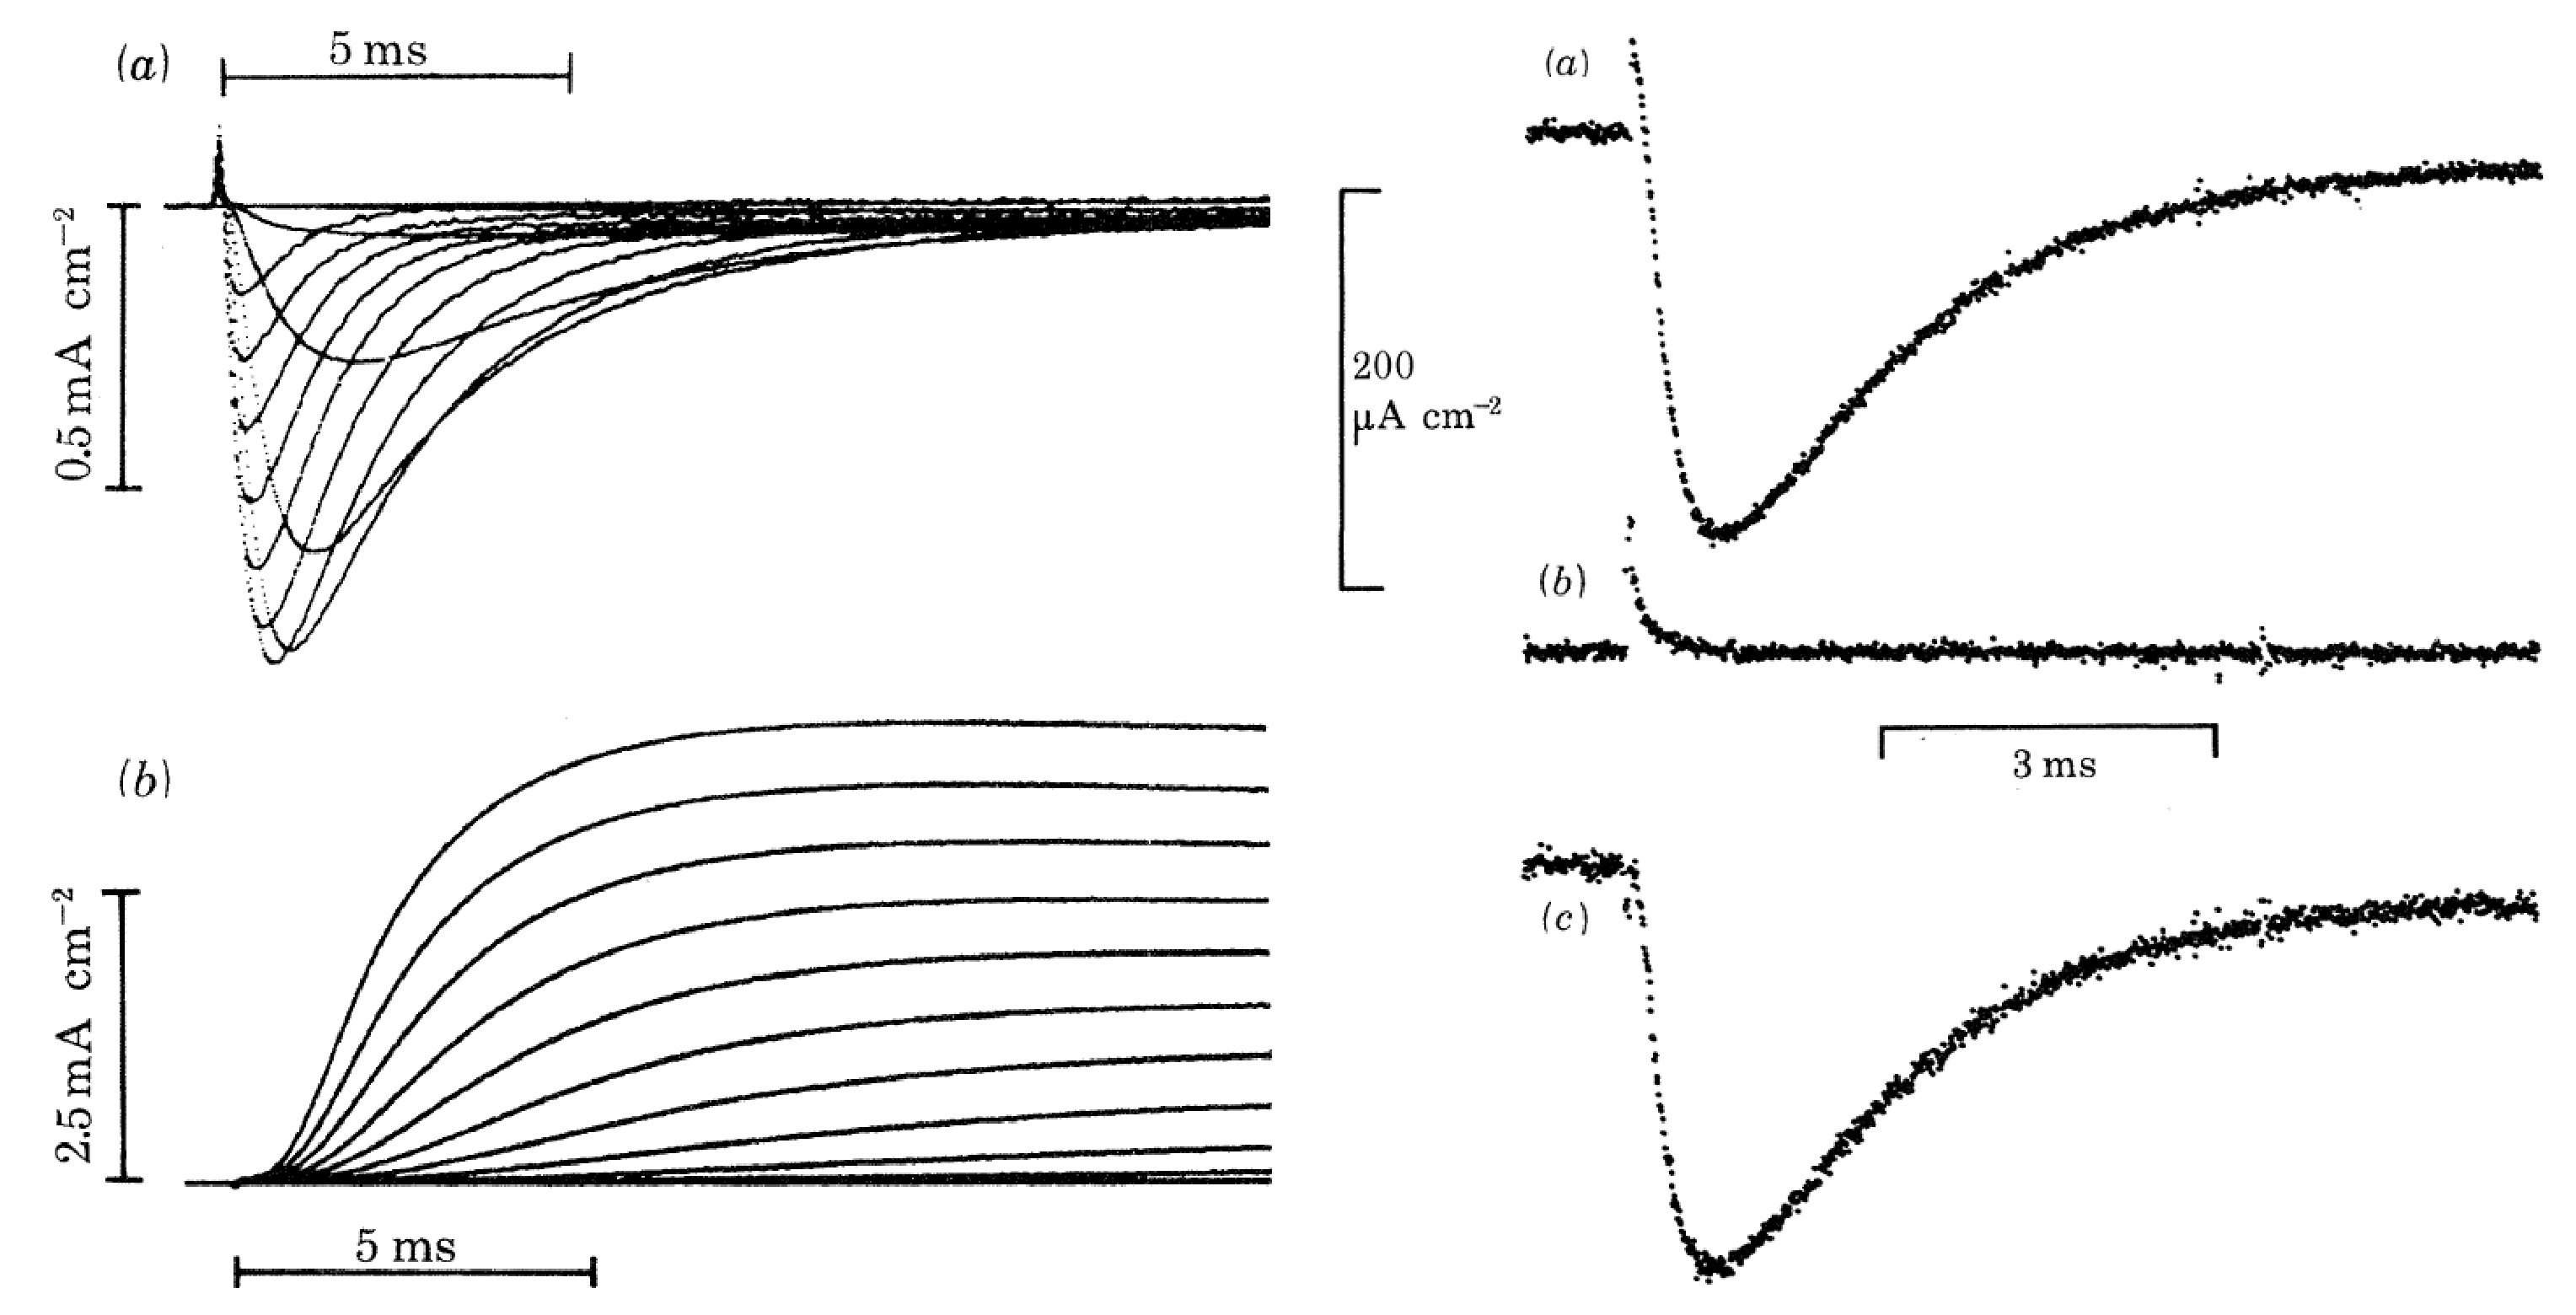
\includegraphics[height=7cm,
    angle=0]{./images/conductance-traces-Na-K.eps}}
  \caption{Conductance traces of (A) sodium current; (B) potassium current at
  different voltage-step values from the same holding potential of -70
  mV; and pulse for each trace increase every 10 mV from -60mV to +60mV. 
  {\it Temperature is 5$^\circ$C}.  Right plots: $I_\na$ current is revealed (c) after subtracting (a) from the
  gating current Ig	(Sect.\ref{sec:gating-current})}
\label{fig:conductance-traces-Na-K}
\end{figure}

\begin{mdframed}

Currents are selectively blocked by (for K+ block) using internal dyalysis with
350mM CsF; and the axon is bathed with $\K$-free artificial sea water containing
103 mM NaCl and 344 mM Tris buffer; (for $\Na$ block) using internal dyalysis
with 350 mM KF; and axon is bathed with artificial sea water containing 1 $\muM$
TTX.
\end{mdframed}


IMPORTANT: At the time recording, the underlying biophysical mechanism
for the two currents was completely unknown, and the data available did not
implicate the existence of a membrane-spanning protein at the site of ion
conduction. However, it is believed that sodium channels and potassium channels
are separate entities existing side by side  in the membrane, as each set can be
blocked completely without affecting the other.

\begin{figure}[hbt]
  \centerline{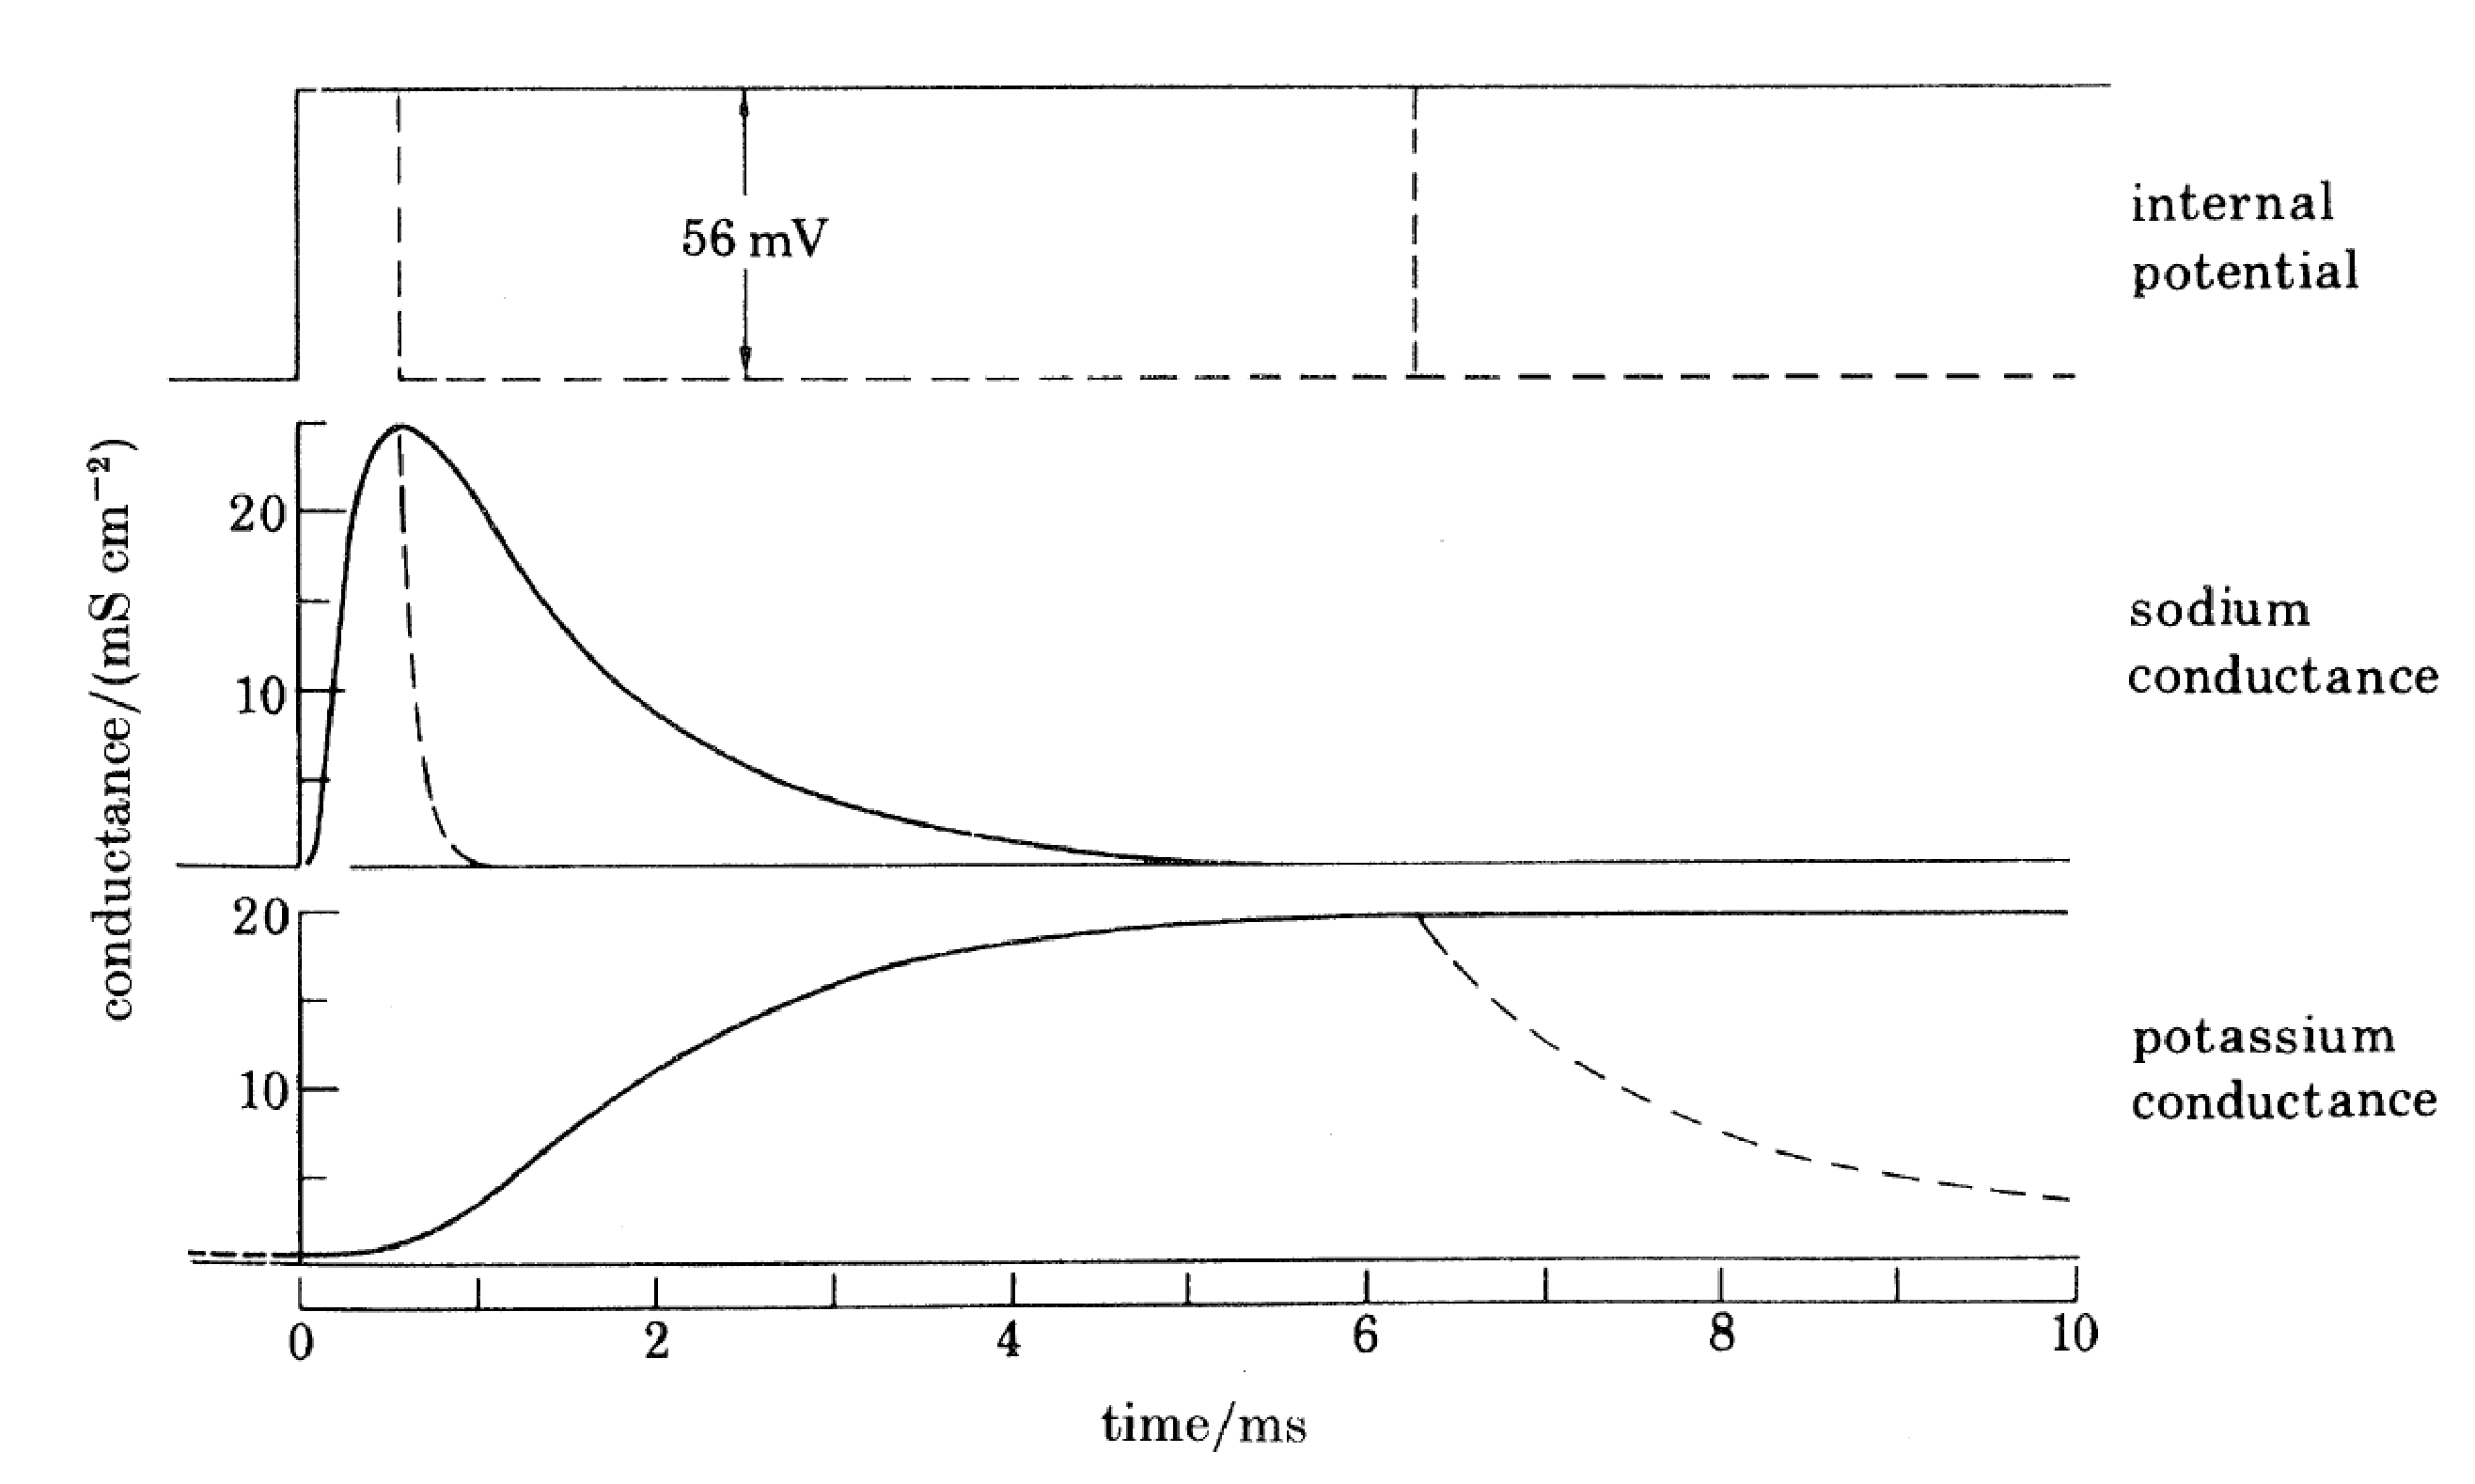
\includegraphics[height=4cm,
    angle=0]{./images/persistent-K-transient-Na.eps}}
  \caption{(A) voltage-clamp with amplitude +56mV (from the holding potential)
  to squid giant axon at 8.5$^\circ$C; (B) $\Na$ current is transient (quickly
  reaches maximum conductance within 0.6ms; and then start to decay); (C) $\K$
  current is persistent (slowly increase to the maximum conductance within
  6.3ms; and then stay at that level); the dash lines shows the kinetics of
  inactivation after the voltage has returned to the holding potential}
\label{fig:persistent-K-transient-Na}
\end{figure}


TAKE HOME MESSAGE: Under voltage clamp, the permeability of the membrane to
sodium and potassium ions undergoes characteristic changes, with different time
courses.
\begin{itemize}
  
  \item sodium conductance rises fairly quickly but not instantaneous (i.e. {\bf
  activation}), with an S-shape; and then fall backs (more slowly) to zero
  through a process known as {\bf inactivation} (even though the depolarization
  is maintained.)
  
  \item potassium conductance rises, slower, but also with a delay; and is not
  inactivated.
  
\end{itemize}
The change in conductance arises under the influence of the electric field
across the membrane (Sect.\ref{sec:electric-field}).


\section{Gating processes: activation, deactivation, inactivation, reactivation}
\label{sec:gating-variables}

\def\deactivation{{\textcolor{red}{deactivation}}}
\def\inactivation{{\textcolor{red}{inactivation}}}
\def\reactivation{{\textcolor{red}{reactivation}}}
\def\activation{{\textcolor{red}{activation}}}

In electrophysiology, the term {\bf gating} refers to the opening (activation)
or closing (by \deactivation or \inactivation) of ion channels.
The name 'gating' derives from the idea that an ion channel protein includes a
pore that is guarded by one gate or several gates, and all the gate(s) must be
in the open position for any ions to pass through the pore.

The gates switch back and forth between open position and closed position, with
a forward rate $\alpha$ and backward rate $\beta$ which are typically
voltage-dependent ($\Vm$ transmembrane potential).

The gates thus can be of the same types (i.e. same kinetics/rates) or different
types (i.e. different kinetics or different rates) which leads to the same or
different {\bf gating processes}.

The rate at which any of these gating processes occurs in response to these
triggers are known as the '{\bf kinetics of gating}.'
\begin{itemize}
  \item Voltage mainly play the role of triggering (opening or closing) the
  gating process.
  
  \item Some drugs and many ion channel toxins act as 'gating modifiers' of
  voltage-gated ion channels by changing the kinetics of gating.
  
  Gating modifier can be (1)  making the process faster or slower; (2)
  changing the steady-state value.
   
\end{itemize}

The gating process can be triggered by the change in one or different factors,
e.g. changes in voltage across the cell membrane (voltage-gated ion channels),
drugs or hormones interacting with the ion channel (ligand-gated ion channels),
changes in temperature,[2] stretching or deformation of the cell membrane,
addition of a phosphate group to the ion channel (phosphorylation), and
interaction with other molecules in the cell (e.g., G proteins).

\textcolor{red}{There are four gating processes}: activation, deactivation,
inactivation, and reactivation (also called 'recovery from inactivation')
\begin{enumerate}
  \item \activation: the process of opening the activation gate, e.g. 'm' gate
  (which occurs during membrane depolarization - for depolarization-activated
  channels).
  
  At rest (hyperpolarized potential), then $m \approx 0$. Upon $\Vm$
  depolarization, then $m \rightarrow 1$ direction with a rate called $\tau_m$.

 Based on the forward rates $\alpha_m$, and backward rate $\beta_m$, the
 steady-state value $m_\infty$, and the time constant $\tau_m$ is 
 \begin{equation}
 \begin{split}
 m_\infty = \alpha_m / (\alpha_m + \beta_m) \\
 \tau_m = \frac{1}{\alpha_m + \beta_m}
 \end{split}
 \end{equation}
 Sect.\ref{sec:fit-activation-HH} describe how to fit $m_\infty$ and $\tau_m$
 from voltage-clamp protocol. 
  
  \item \deactivation: the opposite process of \activation, i.e. the activation
  gate becomes closing, (which occurs during membrane repolarization)
  
 In the opposite direction, i.e. with membrane repolarization, the $m$ gate
 become smaller; yet with a different rate called $\tau_\deact$.
  
 A voltage-clamp protocol needs to bring $\Vm$ to a depolarized value and
 then apply a repolarized voltage pulse which measure the tail current. This
 tails current is a decay current, which reflect how fast $m$ get from the value
 back to zero. This is called deactivation time constant $\tau_\deact$.
  \item \inactivation: the process of closing the inactivation gate
  ($h\rightarrow 0.0$), which occurs in parallel (or may be with a delay) to the 
  \activation (i.e. during membrane depolarization)
  
  Inactivation time course $\tau_h$
  
  \item \reactivation: or recovery from inactivation, i.e. how fast/slow $h$
  gates getting back to 1 (i.e. during membrane repolarization)
  
  
\end{enumerate}
Both inactivation and deactivation are processes that lead to the channel
becoming non-conducting (by blocking different gates); such gates are triggered
by voltage change in different directions; with different rates. So, depending
how slow/fast the change and the direction of the change, it determines channel
gating.
\footnote{\url{https://en.wikipedia.org/wiki/Gating_(electrophysiology)}}


Suppose that the gating of an ion channel is affected by the displacement of
some positive charged {\bf n} ``gating'' variable whose fraction in the
``permissive'' position is $n$ (which affect the channel conductance) and the
fraction in the ``non-permissive'' position is $(1-n)$ - which does not affect
the channel conductance (Sect.\ref{sec:gating-particles}).
%It means that the amount of these agonist/antagonist in both sides is
% conserved.

Given that $n_\infty$ has the sigmoid shape and $\tau_n$ has the bell
shape, a generalized function with 8 coefficients for rate constants
$\alpha, \beta$ is
\begin{equation}
  \label{eq:578}
  \alpha (\text{or } \beta) = \frac{C_0 \exp [C_2(V_m + C_3)] +C_4(V_m +C_5)}{\exp [C_6(V_m +C_3)] + C_7}
\end{equation}
which vary between 0 and 1.

\subsection{In HH model (squid axon)}
%\label{sec:hh-model}

\textcolor{red}{ By using some tools for curve fitting to estimate the
  8 values $C_i$, a clearly good fit to the experimental data, were
  given}
\begin{equation}
  \label{eq:64_copy}
  \begin{split}
    \alpha_n = \frac{0.01 (10-v)}{\exp(\frac{10-v}{10}) - 1}
    \\
    \beta_n = 0.125 \exp(\frac{-v}{80})
  \end{split}
\end{equation}
or
\begin{equation}
  \label{eq:352_copy}
  \alpha_n = \frac{0.01 (V_m+55)}{1-\exp(-\frac{V_m+55}{10})}
  ,
  \beta_n = 0.125 \exp(-\frac{V_m+65}{80})  
\end{equation}

All formulation obtained below for Hodgkin-Huxley model were measured
at $T_c=6.3^\circ$C. If we measure at a different temperature, we need
to adjust the equation by a factor, for every difference in 10 degree
Celcius.
\begin{equation}
  \label{eq:930}
  \frac{dg}{dt} = \Phi \left[ - \frac{g-g_\infty}{\tau_g}\right]
\end{equation}
and
\begin{equation}
  \label{eq:931}
  \Phi=(Q10)^{(T_C-6.3)/10}
\end{equation}
at $T_c=6.3^\circ$C, with a $Q10=3$, thus $\Phi=1$. 

\subsection{-- \ce{K+} channel}
\label{sec:cek+-channel}

\begin{equation}
  \label{eq:59}
  \begin{split}
    g_{\ce{K}} &= \overline{g_K} n^4  \\
    % \frac{dn}{dt} &= \alpha_n \times (1-n) - \beta_n n
  \end{split}
\end{equation}
with $\overline{g_K}$ is the maximum possible conductance, $n$ is a
unitless time-variant quantity.

\subsection{-- \ce{Na+} channel}
\label{sec:cena+-channel}

Then the probability that a channel open is $m^{k_1}h^{k_2}$, with
$k_1,k_2$ are cooperative binding numbers. Using curve fitting
technique, they get $k_1=3,k_2=1$. Then, the probabilities
that a sodium channel is in the permissive position is $m^3h$.
\begin{equation}
  \label{eq:157}
  g_{\ce{Na}} = \overline{g_{\ce{Na}}} m^3 h
\end{equation}
with, similarly, $\overline{g_{\ce{Na}}}$ is a constant (the maximum
conductance when all sodium channels active).  

\begin{equation}
  \label{eq:353_copy}
  \alpha_m = \frac{0.1(V_m+40)}{1-\exp(-\frac{V_m+40}{10})} ,
  \beta_m = 4 \times \exp(-\frac{V_m+65}{18})
\end{equation}
and
\begin{equation}
  \label{eq:354_copy}
  \alpha_h = 0.07\times \exp (-\frac{V_m+65}{20})  ,
  \beta_h = \frac{1}{\exp(-\frac{V_m+35}{10}) + 1}
\end{equation}

\subsection{Noble model (Purkinje fibre)}
%\label{sec:noble-model-1}

\subsection{-- \ce{Na+} channel}
\label{sec:cena+-channel-1}

Shift along the $V_m$ axis by about 20 mV. 
\begin{equation}
  \label{eq:358_copy}
  \begin{split}
    \alpha_h &= 0.17 \exp (-\frac{V_m+90}{20})  \\
    \beta_h &= \frac{1}{\exp(-\frac{V_m+42}{10}) + 1}
  \end{split}
\end{equation}










\section{Hodgkin-Huxley model (1948-1952)}
\label{sec:Hodgkin-Huxley-1952-model}


The BIG question is how an excitable cell maintains a proper gradient of ionic
concentration and cellular homeostasis.  Even before the discovery of
transmembrane proteins serving as pores for ion permeability,  importance of
ionic movements in excitable tissues has been emphasized by a number of recent
experiments \citep{hodgkin1952mcv}.

In the early days, giant squid axon was widely used, and the
electrophysiological of the the axon's transmembrane potential was studied in a
landmark model by Hodgkin and Huxley in 1952, as a result from a series of
papers (Sect.\ref{sec:Hodgkin-Huxley-series-works}). This is the most important
model in the course of computational cell biology \citep{hodgkin1952ap}. The
model was described in the last paper of the series of 5 papers in 1952 by
Hodgkin and Huxley .


\subsection{Theoretical background and assumptions in Hodgkin-Huxley
formula?}
\label{sec:Hodgkin-Huxley-hypothesis}

{\bf HYPOTHESIS 1}:  An early view of the hypothesis for sodium permeation in
that sodium ions do not move by themself; but combined with lipoid soluble
carrier. Such carriers bears a large negative charge and can combine with one
sodium ion but no more (as suggested in Hodgkin, Huxley, Katz (1949)). However,
this hypothesis was rejected.

{\bf HYPOTHESIS 2}:  Another view (also rejected) is that only one system is
present which permeate to sodium first; and its selectivity changes (to potasium) soon after the
membrane is depolarizes. However, this hypothesis cannot be applied in a simple
form since the potassium conductance rises too slowly for a direct conversion
from a state of sodium permeability to one of potassium permeability.

{\bf HYPOTHESIS 3}:  Hodgkin and Huxley (1952) then utilized the hypothesis that
there are two separate systems: one selectively permeate to sodium; and one
selectively permeate to potassium. 
\begin{enumerate}
  \item sodium-system - Sect.\ref{sec:cena+-conductance}
  
  Here, sodium movement across the membrane depends on the distribution of
  charged particles (gating particles) which do not act as carriers (as similar
  that in hypothesis 1) but allow sodium to pass through the membrane when they
  occupy particular sites in the membrane. So, the rate of movement of the
  activating particles determines the rate at which the sodium conductance
  approaches its maximum but has little effect on the magnitude of the
  conductance. 
  
  \item potassium-system - Sect.\ref{sec:cek+-conductance}

A similar mechanism applies to potassium-system.

\end{enumerate}




\subsection{-- gating particles}
\label{sec:gating-particles}

To explain the change in the conductance of $\Na$ and $\K$ ions species,
Hodgkin-Huxley proposed a hypothesis that the voltage gradient across the
biomembrane forms a dipole and that any voltage-gated channels have charged
voltage-sensor built into the channels. The strength of the dipole and electric
fields it generates control how the permeability of the ions across the
membrane by translocate these charged voltage-sensor domains.

It is assumed that there are some particles (with positive charges) that at {\it
resting state}; can bring positive charges close enough to the channel's pore to
block or prevent any cations  from penetrating the biomembrane.
These particles serve as {\bf gating particles}; and the channel open when and
only when the gating particles flipped to their {\it Open state}.

There are two types of gating variables (particles): {\it activating gates} and
{\it inactivating gates}.
\begin{enumerate}
  \item a particle (gating variable) has two states: resting state or activated
  state. 
  
NOTE: Some later models can use more than 2 states
    
  \item a potassium channel whose conductance is controlled by a few activating gates.
  
  Hodgkin-Huxley proposed 4 activating gates that need to be
  translocated for the channel to open, i.e. the fraction of opening channel at
  a time is the fraction that all 4 activating gates are in Open state, i.e.
  $n^4$.
  
  
  \item a sodium channel whose conductance is controlled by a few 
  activating gates; and a few inactivating gates.
  
  
  Hodgkin-Huxley proposed 3 activating gates and 1 inactivating gate that need
  to be translocated for the channel to open. The fraction of opening channel at
  a time is $n^3 \times h$.
  
%   
%   However, there is another single
%   {\bf h} particle that once translocated, it blocks the channel. The
%   translocation for {\bf h} particle is slower, and occurs at the same time
%   (i.e. independent) from the translocation of {\bf m} particle.
%   
\end{enumerate}
The gating particles do not act as charged carriers and is not
voltage-dependent, but its function is to allow ions, for example: sodium, to
pass-through the membrane when these gating particles translocate to the
'permissive' position. 

On this view, then the {\bf rate of movement} of this gating m-particle $dm/dt$,
upon voltage change (i.e. $m=m(\Vm)$), determine the {\bf rate} at which $\Na$
conductance approaches its maximum; but not the value of the maximum
conductance. So, temperature only has effect on the rate (or the time constant
$\tau_m$).

\begin{mdframed}
NOTE: Here we use interchangebly the name of the particle, e.g. $m$, and the
fraction of such particle in the inner membrane, i.e. $m$.
\end{mdframed}


\subsection{\texorpdfstring{\ce{Na+} conductance}{Na+ conductance}}
\label{sec:cena+-conductance}

Based on the accepted hypothesis 3 given in
Sect.\ref{sec:Hodgkin-Huxley-hypothesis}, it is assumed that the sodium
conductance depends upon the concentration of such sodium-sensitive gating
particles on the inside of the membrane (proportion: $P_i$); but is independent
of the number of such gating particles on the outside (proportion: $P_o$). NOTE:
The total number of such gating particles are assumed to be constant; but they
can translocate across the membrane.

The Boltzmann's principle allows us to estimate the proportion $P_i/P_o$
\begin{equation}
\frac{P_i}{P_o} = \exp \left[ \frac{w - z.e.\Vm}{k_BT} \right]
\end{equation}
with $\Vm$ is transmembrane potential (inside-outside); $w$ is the work required
to move the gating particles from inside to outside when $\Vm = 0$.; $e$ is the
absolute value of the electronic charge; $z$ is the valance of the charged
gating variables. Since $P_i + P_o = 1$, then

\begin{equation}
P_i = \frac{1}{1 + \exp\left[ - \frac{w - z.e.\Vm}{k_BT} \right]}
\end{equation}
A good approximation (when $z$ is negative, and $\Vm$ is sufficient negative)
\begin{equation}
P_i = \text{ constant } \times \exp\left( -ze\Vm/(k_BT) \right)
\end{equation}

As $g_\na$ increase e-fold by the depolarization of only 4 mV; i.e.  $g_\na
\propto \exp(\Vm/4)$. To explain such result, $z$ must be about -6; since
$\frac{k_BT}{z}=\frac{RT}{F} \approx 25 $(mV), which gives
\begin{equation}
g_\na \propto \exp(\Vm/4.17)
\end{equation}
Based on such analysis, Hodgkin and Huxley suggested that the charged gating
particle must bear six negative electronic charges (i.e. $z=-6$); or if an alternate hypothesis (long molecule
with a dipole moment) is used; the charged long molecule must have 3 negative
charges on one-end and 3-negative charges on the other end.

The proportion of the time that each of the charged particle spend at the inside
is determined by $\exp(\Vm/25)$; so the proportion of sites at which all 6 are
at the inside is $\exp(\Vm/4.17)$.
HERE: sodium movement is assumed to depend on the presence of six singly charged
particles at a particular site near the inside of the membrane.

\subsection{-- activation and inactivation}

The voltage-clamp data showed a biphasic behavior in sodium conductance: rising
phase, and then decay. There are two mathematical methods for describing this
behavior
\begin{enumerate}
  \item assume that the sodium conductance is determined by a variable which
  obeys a second-order differential equation.

  \item it is determined by two variables, each of which obeys a first-order
  equation: one trigger the opening and one trigger the closing.
  
  Again, it is assumed that the conductance of sodium is depending the
  proportion of these two types of gating particles on the inside of the
  membrane for the activating particle; and on the outside of the membrane for
  the inactivating particles. The proportions are called $m$ for activating
  particles (inside); and $h$ for inactivating particles (outside). At resting
  potential: $m$ is small; while $(1-h)$ is small. Depolarization helps increase
  $m$ (faster); and increase $(1-h)$ (slower).
  
  
\end{enumerate}
The second mechanism was chosen since it was simpler. 


% \subsection{-- Mathematical model}
% \label{sec:mathematical-model-1}

%\subsection{-- Build the hypothesis}
%\label{sec:build-hypothesis}

\subsection{-- conductance}
\label{sec:conductance-Na+-current-HH}

Based on the result in the third paper
(Sect.\ref{sec:Hodgkin-Huxley-third-paper}), the ionic current is assumed Ohm's law
\begin{equation}
I_{\Na} = g_{\Na} \times (\Vm - E_{\rev,\Na})
\end{equation}

\begin{figure}[htb]
  \centerline{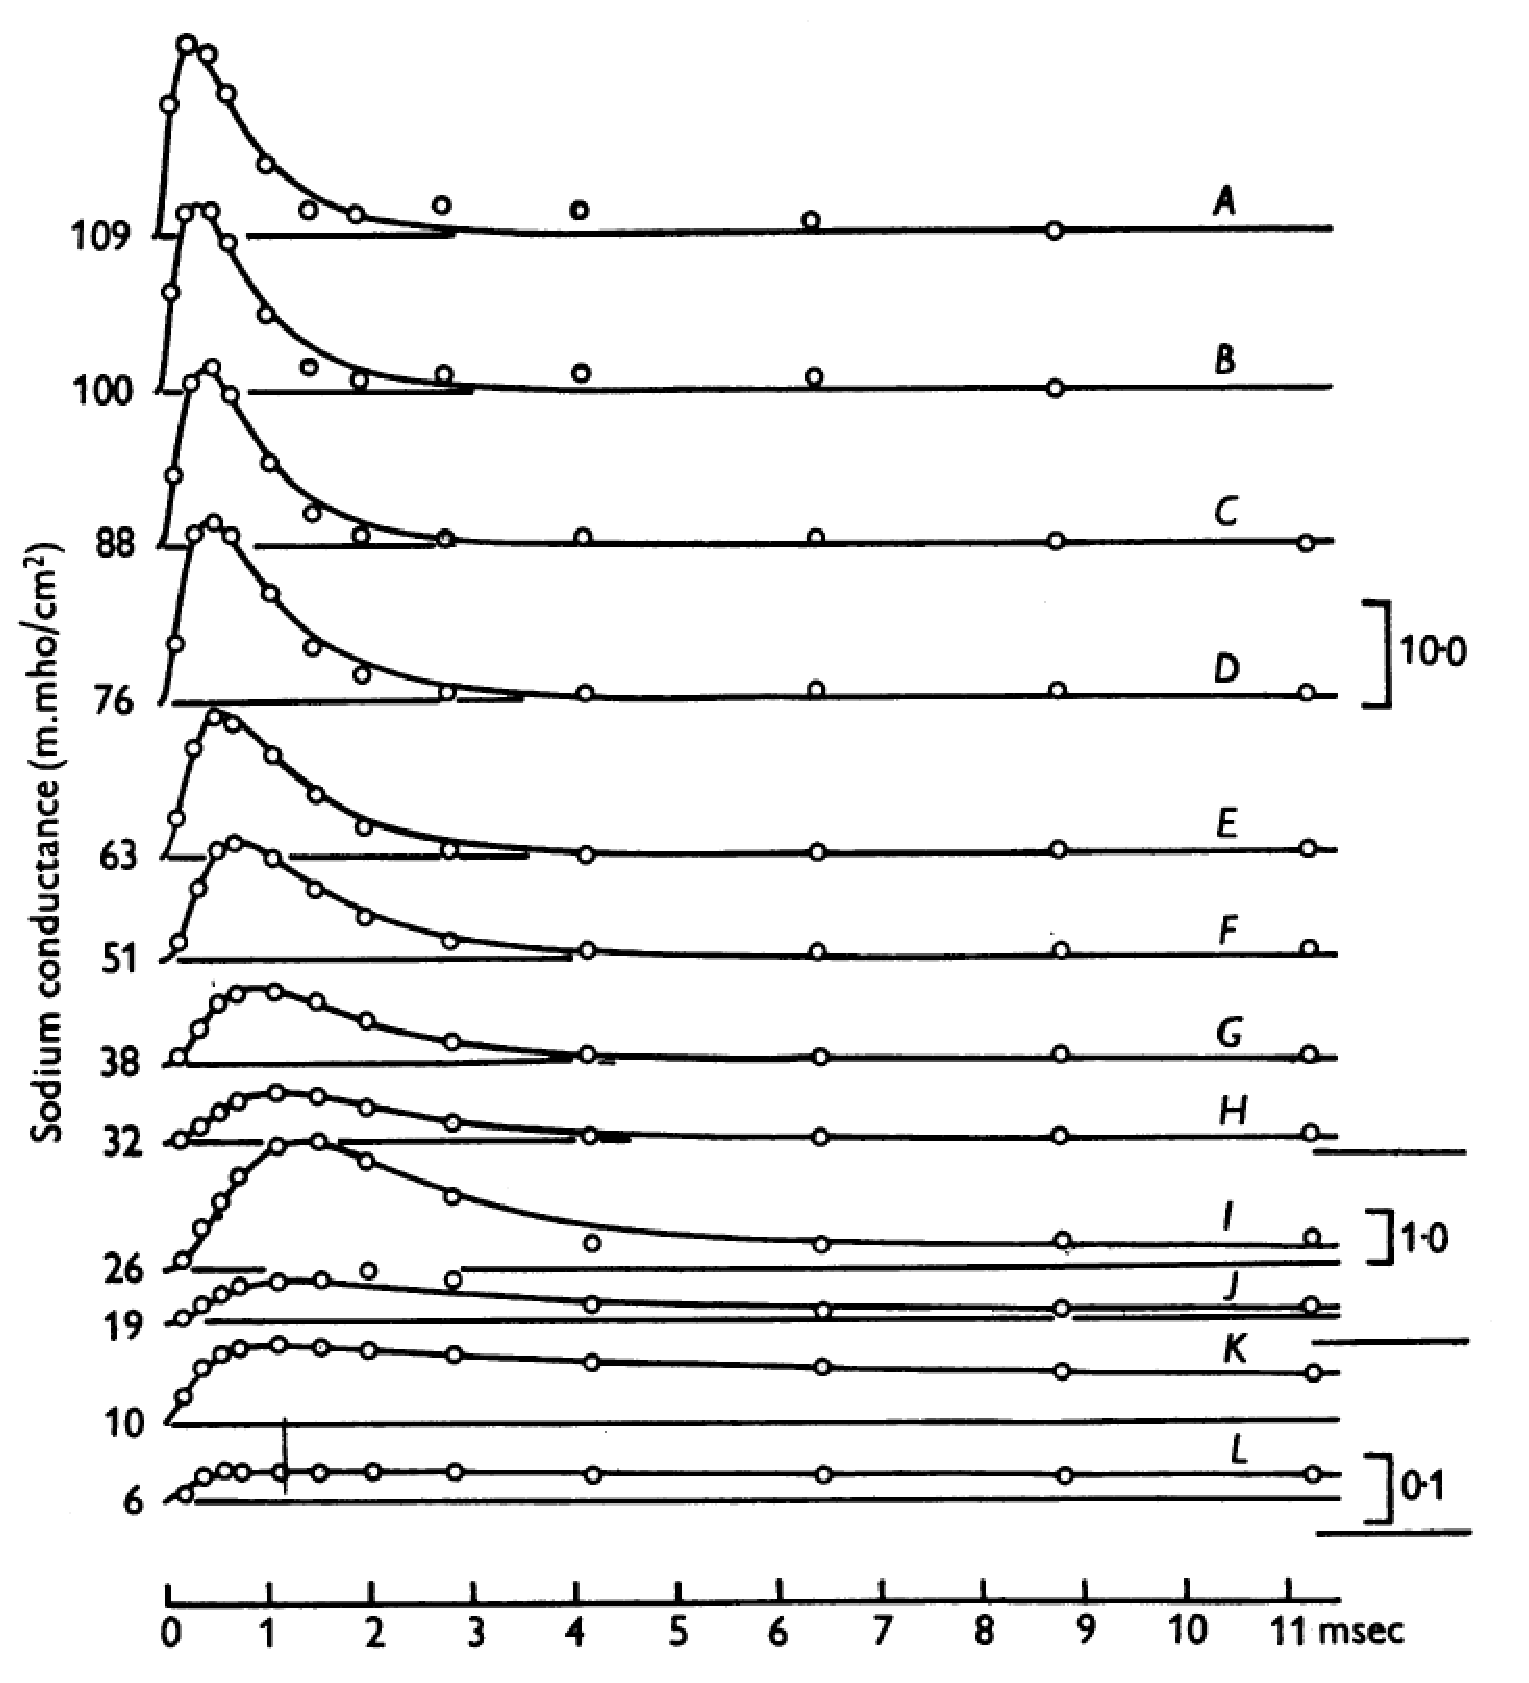
\includegraphics[height=7cm]{./images/sodium-conductance-HH.eps}}
  \caption{Changes of sodium conductance with
  different conditioning potentials [NOTE:
  The inward current is showed positive due
  to old convention]}\label{fig:sodium-conductance-HH}
\end{figure}

There have to be 2 kinds of gating particles:
{\it activating particles} ($m$) and {\it inactivating particles}
($h$); with $m$ is the proportion of the activating particle on the inside
of the membrane (i.e. the probability that it binds to \ce{Na+} channel, while
\textcolor{red}{$h$ is the probability that a \ce{Na+} channel is NOT
  bound by the inactivating particle}.

The fraction of opening channels is $m^{k_1}h^{k_2}$, with
$k_1,k_2$ are cooperative binding numbers. Using curve fitting
technique, they get $k_1=3,k_2=1$. Then, conductance is written as
\begin{equation}
  \label{eq:157}
  g_{\ce{Na}} = \overline{g_{\ce{Na}}} m^3 h
\end{equation}
with, similarly, $\overline{g_{\ce{Na}}}$ is a constant (the maximum
conductance when all sodium channels active).  \textcolor{red}{The analytical
solution is discussed in
Sect.\ref{sec:conductance-Na+-current-HH-analytical-form}}

\begin{mdframed}

Hodgkin and Huxley chose  $m$ raised to $k_1=3$ to account for the delay in
the rise of $g_{\ce{Na}}$. The meaning of $m$ and $h$ is equivalently to the
normalized concentration of such activating/inactivating particles
in the cytoplasm.  
  
$m$ reflects the fraction of activation ``particles'' which occupy a
``permissive position'' (one tending to open channels and thus increase
$g_{\ce{Na}}$; $h$ is the fraction of inactivation particles in the permissive
position. Conversely, $(1-h)$ and $(1-m)$ are fractions of particles in the
alternative, non-permissive, position.

  The distribution of the activating/inactivating ``particles''
  determine the rate at which the sodium conductance reach its
  maximum, but has little effect on the magnitude of the maximum
  value.  The rate of increase $m$ with time is equal to amount of
  activation ``particles'' move to the permissive position (with rate
  $\alpha_m$) minus the amount of activation ``particles'' move to the
  non-permissive position (with rate $\beta_m$). Similarly, for the
  case of inactivation ``particles''.
  \begin{equation}
    \label{eq:826}
    \begin{split}
      \text{(m)} \ce{<=>[\beta_m][\alpha_m]} \text{(1-m)} \\
      \text{(h)} \ce{<=>[\beta_h][\alpha_h]} \text{(1-h)} \\
    \end{split}
  \end{equation}

  and the change in the fraction of activation/inactivation
  ``particle'' in the permissive position are given as
\begin{equation}
  \label{eq:65}
  \begin{split}
    \frac{dm}{dt} &= \alpha_m \times (1-m) - \beta_m m \\
    \frac{dh}{dt} &= \alpha_h \times (1-h) - \beta_h h
  \end{split}
\end{equation}
with all $\alpha,\beta$ are rate-constant which are indeed functions
of voltage ($V_m$), but NOT of time.
\end{mdframed}

% $m$, $(1-h)$ represent for the proportions of activating particles,
% and inactivating particles, respectively, on the inside the cell.
% $(1-m)$, $h$ are the proportions of activating particles and
% inactivating particles, respectively, on the outside. 
% \begin{equation}
%   \label{eq:158}
%   \begin{split}
%      "1-m" &\ce{<=>[\alpha_m][\beta_m]} m \\
%      "1-h" &\ce{<=>[\alpha_h][\beta_h]} h \\
%   \end{split}
% \end{equation}
\subsection{-- derive 'm', 'h'}

The HH model treats the activation and inactivation processes in sodium
channels as entirely independent of each other; with both depend on membrane
potential $\Vm$.

For the resting potential (at time $t=0$), we get $m=m_o$; $n=n_o$.

Similar to eq.~\eqref{eq:61}, given the two
boundary conditions $m_0$, $h_0$ at $t=0$, the explicitly solution for
$m$ and $h$ are
\begin{equation}
  \label{eq:66}
  \begin{split}
    m = m_\infty - (m_\infty - m_0) \exp (-t/\tau_m) \\
    h = h_\infty - (h_\infty - h_0) \exp (-t/\tau_h) 
  \end{split}
\end{equation}
with
\begin{equation}
  \label{eq:67}
  \begin{split}
      m_\infty = \alpha_m /(\alpha_m + \beta_m); \tau_m =
  \frac{1}{\alpha_m+\beta_m} \\
  h_\infty = \alpha_h /(\alpha_h + \beta_h); \tau_h =
  \frac{1}{\alpha_h+\beta_h} \\
  \end{split}
\end{equation}

\subsection{-- analytical form of conductance}
\label{sec:conductance-Na+-current-HH-analytical-form}

We then substitute them into eq.\ref{eq:157}, 
\begin{equation}
\label{eq:HH-Na-conductance-exact-form}
g_\na = \bar{g}_{\na} \times \left( m_\infty - (m_\infty - m_0) \exp
(-t/\tau_m) \right)^3 \times \left( h_\infty - (h_\infty - h_0) \exp
(-t/\tau_h)\right)
\end{equation}

This function is quite complicated to be solved, so a simplified form is used by
Hodgkin and Huxley -
Sect.\ref{sec:conductance-Na+-current-HH-analytical-form-simplified-formed}.

\subsection{-- simplified analytical form of conductance}
\label{sec:conductance-Na+-current-HH-analytical-form-simplified-formed}

For the assumptions below to be used with small error, only traces
A-H are used to fit the data.

ASSUMPTIONS:
\begin{itemize}
  
  \item at resting state (or at holding potential $V_\text{ps}$ (pre-step)):
  conductance of sodium is very small compared to large depolarization: so at
  large depolarization ($\Delta V >30$ mV); we can assume to ignore $m_o$.

  
  \item also, at large depolarization ($\Delta V > 30$mV), the inactivation is
  nearly completed, i.e.  $h_\infty \approx 0$; so $h_\infty$ can be neglected.
  
\end{itemize}

So, a shorter (simplified) analytical form of sodium conductance
% \begin{equation}
% \label{eq:HH-Na-conductance-reduced-form}
% \begin{split}
% g_\na  &\approx \bar{g}_{\na} \times \left( m_\infty - (m_\infty ) \exp
% (-t/\tau_m) \right)^3 \times \left( 0 - ( 0 - h_0) \exp
% (-t/\tau_h)\right) \\ 
%  &\approx \bar{g'}_{\na} \times \left( 1 - \exp
% (-t/\tau_m) \right)^3 \times \left(\exp
% (-t/\tau_h)\right)
% \end{split}
% \end{equation}
\begin{equation}
g_\na  \approx \bar{g}_{\na} \times \left( m_\infty - (m_\infty ) \exp
(-t/\tau_m) \right)^3 \times \left( 0 - ( 0 - h_0) \exp
(-t/\tau_h)\right)  
\end{equation}
or
\begin{equation}
\label{eq:HH-Na-conductance-reduced-form}
g_\na  \approx
\bar{g'}_{\na} \times \left( 1 - \exp(-t/\tau_m) \right)^3 \times \left(\exp
(-t/\tau_h)\right)
\end{equation}
with $\bar{g'}_{\na} = \bar{g}_{\na} \times (m_\infty)^3 \times h_0$ is the
peak sodium conductance at each conditioning potential.

NOTE: $m_\infty$ is the final activation reached; and $h_0$ is the initial
inactivation level. 

\subsection{-- estimate time-constant 'tau-m', 'tau-h'}
\label{sec:estimate-tau-m-tau-h-HH}

The analytical form of the sodium conductance eq.\ref{eq:HH-Na-conductance-reduced-form}
(when $\Delta V > 30$mV, i.e. traces A-H in Fig.\ref{fig:sodium-conductance-HH})
is used to fit with the voltage-clamp data, from that the time-constants
$\tau_m$ and $\tau_h$ can be found.

For traces I-L in Fig.\ref{fig:sodium-conductance-HH} (when depolarization is
small, i.e. less than 30 mV in amplitude), Hodgkin and Huxley assumed $h_\infty$
and $\tau_h$ had values calculated from experiment described in their third
paper (Sect.\ref{sec:Hodgkin-Huxley-third-paper}).

\subsection{-- estimate 'm-infty'}

It is assumed that $m$ change much faster than $h$, so when $m$ reaches the
peak, $h$ has not changed much, so the value of $m_\infty$ is estimated from
\begin{equation}
m_\infty \approx \left( g'_{\na} \right)^{1/3}
\end{equation}


This is equal to
\begin{equation}
m_\infty = \frac{\alpha_m}{\alpha_m + \beta_m}
\end{equation}
with $\alpha_m, \beta_m$ are derived from the method given below.


\subsection{-- estimate 'alpha-m', 'beta-m'}


{\bf Formulate $\alpha_m$ and $\beta_m$}: we use the similar procedure
that was used with $\alpha_n$ and $\beta_n$. 
\begin{equation}
\begin{split}
\alpha_m = \frac{m_\infty}{\tau_m} \\
\beta_m = \frac{1- m_\infty}{\tau_m}
\end{split}
\end{equation}

All data were collected from different temperatures, and then reduced to
6$^\circ$C by adopting a Q10 of 3 (Sect.\ref{sec:q10-factor}). 

Plotting the experimental
data points against the membrane potential $v=\Vm - V_\rest$, the fitting curves
are given

% \begin{equation}
%   \label{eq:69}
%   \alpha_m = \frac{m_\infty}{\tau_m}; \beta_m = \frac{1-m_\infty}{\tau_m}
% \end{equation}

\begin{equation}
  \label{eq:70a}
  \begin{split}
      \alpha_m &= \frac{0.1(25-v)}{\exp(\frac{25-v}{10})-1} \\
      \beta_m &= 4 \exp(\frac{-v}{18})
  \end{split}
\end{equation}
with [$\beta_m$]=[$\alpha_m$]=ms$^{-1}$, [$v$]=mV.
The equivalent formula of eq.~\eqref{eq:70a} is
\begin{equation}
  \label{eq:353}
      \alpha_m = \frac{-0.1(V_m - (-40))}{\exp(-\frac{V_m - (-40)}{10})-1} ,
      \beta_m = 4 \times \exp(-\frac{V_m - (-65)}{18})
\end{equation}


\subsection{-- estimate 'h-infty'}

The smooth curve of $h_\infty$ is estimated
\begin{equation}
h_\infty = \frac{\alpha_h}{\alpha_h + \beta_h}
\end{equation}

When $\Delta V > 30$ mV, a simpler expression is used
\begin{equation}
h_\infty = \frac{1}{1 + \exp\left( \frac{\Vm - V_h}{7} \right)}
\end{equation}
with $V_h=-2$ (mV) is the potential at which $h_\infty = 0.5$.

\subsection{-- estimate 'alpha-h', 'beta-h'}

\begin{equation}
\begin{split}
\alpha_h = \frac{h_\infty}{\tau_h} \\
\beta_h = \frac{1- h_\infty}{\tau_h}
\end{split}
\end{equation}


{\bf Formulate $\alpha_h$, and $\beta_h$}: The rate constant for the
inactivation process were fitted with the experimental data against
the membrane potential $v_m$
\begin{equation}
  \label{eq:72a}
  \begin{split}
      \alpha_h = 0.07 \exp (\frac{-v}{20})  \\
      \beta_h = \frac{1}{\exp\frac{30-v}{10} + 1}
  \end{split}
\end{equation}
The equivalent form of eq.~\eqref{eq:72a} is
\begin{equation}
  \label{eq:354}
      \alpha_h = 0.07\times \exp (-\frac{V_m - (-65)}{20})  ,
      \beta_h = \frac{1}{\exp(-\frac{V_m - (-35)}{10}) + 1}
\end{equation}
% calculated from
% \begin{equation}
%   \label{eq:71}
%     \alpha_h = \frac{h_\infty}{\tau_h}; \beta_h = \frac{1-h_\infty}{\tau_h}
% \end{equation}

In the resting state, unlike \ce{K+} channels, \ce{Na} channels are
mostly inactivated, therefore $m_0$ is neglected. At infinity, most
channels should have been activated, then $h_\infty$ is neglected. As
the result, the expression for the \ce{Na+} conductance is
\begin{equation}
  \label{eq:68}
  g_{\ce{Na}} = g'_{\ce{Na}} \left[ 1 - \exp (-t/\tau_m) \right]^3 \exp (-t/\tau_h) 
\end{equation}
with $g'_{\ce{Na}} = \overline{g_{\ce{Na}}} m_\infty^3 h_0$.

{\bf QUIZZ}: Derive eq.~\eqref{eq:68}.


\subsection{-- gating current (Ig, I-gate)}
\label{sec:gating-current}

Consider the example of sodium channel whose conductance pore is controlled by
some positive-charged segments (known as particles):
As the channel open, before any inward sodium current occur, there is a small,
transient outward current known as Ig. This a {\bf small, transient gating
current} (Ig) flows outward as the channel gate opens, inward as it closes. 
Even it was predicted by Hodgkin-Huxley in 1952,  actual measurement of these
small currents occurred only 20 years later (Armstrong and Bezanilla, 1973).
and is called capacity current (Sect.\ref{sec:capacitive-current}).

% The flipping over of the positive-charged {\bf m} particles (to a position that
% enable the ion flux through the channel) correspond to an outward movement of
% positive charge, i.e.
% generating a small outward currents that precedes the inward flows of sodium
% current after the channel has opened. This outward current, generated before any
% channel opening, is called {\bf gating currents}. 

So, gating current (for sodium channel) is the outward current generated by the
movement of these charged gating particles (Sect.\ref{sec:gating-particles}),
independent of the presence of the sodium ions.
\footnote{\url{http://www.scholarpedia.org/article/Gating_currents}}
Ig starts before $I_\na$; and continues until all the V-gate are open.

%IMPORTANT: I-g is not voltage-dependent; and does not generate any 


Example: As shown in Fig.\ref{fig:conductance-traces-Na-K} (right column), (a)
trace of $I_\na$ and $I_g$; (b) $I_g$ recorded alone; and (c) $I_\na$ after
subtracting (b) from (a).


% there exists some 'gating' particles,
% e.g. $m$ (for $\Na$ channel) and $n$ (for $\K$ channel), that the movement of
% ions like $\Na$ or $\K$ depends on the binding such gating particles to the
% associated sites, i.e. the site at which $\Na$ pass-through for example.

% The gating particles do not act as charged carriers, but its function is to
% allow sodium ions to pass-through the membrane when these gating particles
% occupy a particular site on the membrane. Suppose the site of the binding is on
% the inner-side of the membrane, and the total of number of gating variable on
% both sides of the membrane is constant; then $m$ represent the fraction of
% gating particle triggering $\Na$ conductance on the inner side, and the

\begin{itemize}  
  \item  sodium conductance is written as $\bar{g_\na} m^p$ with $p$ is the number of
binding sites required for such gating particle.
  
  \item potassium conductance is written as $\bar{g_\k} n^q$ with $q$ is the
  number of binding sites required for such gating particle.
  
\end{itemize}



\subsection{\texorpdfstring{\ce{K+} conductance}{K+ conductance}}
\label{sec:cek+-conductance}

\begin{mdframed}
\textcolor{red}{Early works found $\K$ channels display current in outward
direction} at depolarized $\Vm$, i.e.  responsible for repolarizing a cell following an
action potential. Nowadays, there are many more different types of $\K$
channels. The early model by Hodgkin-Huxley didn't inspected the complex details
of different $\K$ channels (Chap.\ref{chap:potassium-channels}), and thus
kinetics estimate for this $\K$ channel is an approximation of an (outward)
delayed-rectifier $\K$ current (Kdr - Sect.\ref{sec:KDR-Hogkin-Huxley-1952}).

In order to study the behavior of \ce{K+} channels in isolated,
blocking agents were used to inhibit the activities of all types of
channels, except \ce{K+} channels, the conductivity of potassium
channels $g_{\ce{K+}}$ is recorded over time. 

\end{mdframed}

Much of what has been assumed about the changes in sodium permeability
(Sect.\ref{sec:cena+-conductance}) applies equally to the mechanism underlying
the change in potassium permeability.
\begin{enumerate}
  \item activating particles for potassium system have affinity for potassium
  but not sodium
  
  \item these activation particles move more slowly that those in sodium system
  
  \item these activation particles are not blocked or inactivated
\end{enumerate}

\subsection{-- rising and falling conductance}
\label{sec:HH-K+-rising-falling}

As shown in Fig.~\ref{fig:Sodium-Potassium} and the first half of
Fig.~\ref{fig:g_K}, the conductance-voltage $g$-V curves (or $f-V$ curve, with
$f$ is fraction of opening channel) show a sigmoid shape. The depolarization
process shows a single activation gate with a delay (S-shaped time course).  The
hyperpolarization process shows a single deactivation gate (inactivation) with
no appreciable inflexion.

%. This stage, however, follows an exponential
%distribution.

If the conductance $g_K$ is used as a variable, then the activation curve can
NOT be fitted by a first-order equation, but a third- or fourth-order equation
of a variable (e.g. $n$) that obeys the first-order equation. Such third- or
fourth-order equation is needed to describe the 'delay' at the beginning. The
rising in Fig.\ref{fig:g_K} is fitted with
\begin{equation}
\left( 1 - \exp(-t) \right)^4
\end{equation}
NOTE: Better agreement might have
been obtained with a fifth or sixth power, but the improvement was not considered
to be worth the additional complication.

If $g_K$ is used as a variable, then the falling in conductance following
the repolarization can be fitted by a first-order equation, i.e. single
exponential decay. The decaying in Fig.\ref{fig:g_K} is fitted with
\begin{equation}
\left( \exp(- 4 t) \right)
\end{equation}



\begin{figure}[htb]
  \centerline{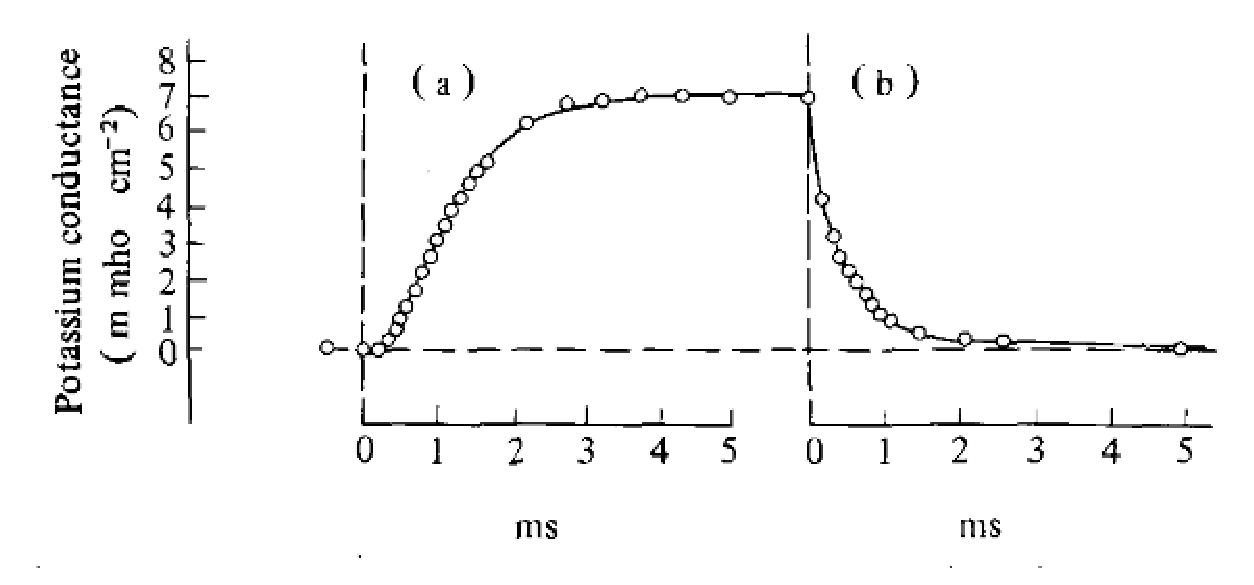
\includegraphics[height=5cm]{./images/g_K.eps}}
  \caption{(a) rise of potassium conductance during depolarization
    (with depolarization +25 mV from resting potential), (b) fall of potassium
    conductance during repolarization (back to resting potential).
    NOTE: the end of (a) is the same as the starting point of
    (b)}\label{fig:g_K}
\end{figure}

The ``activation'' with a delay of \ce{K+} channel could be
interpreted as a multistep process which requires the sequential binding of
more than one (activation) gating charged particles.

% of different closed states before an opening
% state is reached.
% So, \textcolor{red}{a validated hypothesis postulated by Hodgkin and
%   Huxley is that there are a number of activation binding sites on the
% inner side of the $\K$ channels, and the activation of a single \ce{K+} channel
%   requires the binding of some {\it activating particles} $A$ to all
%   of these sites}.

NOTE: The activating particles are not necessary real molecules, just
``hypothesized'' ones that trigger the opening of \ce{K+} channels when
``binding'' to the receptors of \ce{K+} channel.  The higher the concentration
of these binding molecules in the intracellular side, the less time to have more
channels open. Again, the gating is assumed control by these particles on one
side only.


\subsection{-- conductance}
\label{sec:conductance-K+-current-HH}

\begin{mdframed}

\begin{eqnarray}
  \label{eq:555}
  \ce{C <=>[kA][] O}
\end{eqnarray}
With the idea in mind that the activation of a single \ce{K+} channel
requires the proper binding of k independent activators $A$. Suppose
that the probability for an activating particle $A$ to bind to is $p$
($0\le p \le 1$). Then, the probability for the reaction to occur,
i.e. $k$ molecules of $A$ to bind to the channel, is $p^k$. The
question is how to choose the value of $k$ which is now called the
{\bf cooperative binding number}?  Interestingly, if $p$ rises
exponentially from zero to 1 and $k=4$, $p^4$ rises along an S-shaped
curve, imitating the delay increase of $g_{\ce{K}}$ on depolarization;
and if $p$ decreases exponentially to zero, $p^4$ falls exponentially
to zero, imitating the decrease of $g_{\ce{K}}$ on hyperpolarization.

But we still don't know $p$? Luckily, this can be resolved using the
law of conservation, i.e. the total number of agonists $A$ at
intracellular and extracellular doesn't change at all. However, $A$
can move from intracellular to extracellular and vice versa. This
movement is $V_m$-dependent, i.e. $p(V)$.

So, the probability $p$ for an activating particle to bind to the
channel can be considered as the normalized concentration $n$ of the
activating particles in intracellular
medium\footnote{$(1-n)$ is the extracellular concentration of the
  activating particles}
($0\le n \le 1$).  You can ask why we don't consider $n$ as the
normalized concentration in the extracellular? - The answer is that
it's doesn't make any difference, it's just a convention.

\end{mdframed}

Based on the result in the third paper
(Sect.\ref{sec:Hodgkin-Huxley-third-paper}), the ionic current is assumed Ohm's
law
\begin{equation}
I_{\K} = g_{\K} \times (\Vm - E_{\rev,\K})
\end{equation}

Based on the reason in Sect.\ref{sec:HH-K+-rising-falling}, the dynamics of
conductance (at a given value of $\Vm$ and time) is described with, in that the
binding of 4 gating particles is required for conducting potassium ions

\begin{equation}
\label{eq:59}
\begin{split}
g_K &= \bar{g}_K \times n^4 \\
\frac{dn}{dt} &= \alpha_n (1-n) - \beta_n n
\end{split}
\end{equation}
% \begin{equation}
%   \label{eq:59}
%   \begin{split}
%     g_{\ce{K}} &= \overline{g_K} n^4  \\
% %      \frac{dn}{dt} &= \alpha_n \times (1-n) - \beta_n n
%   \end{split}
% \end{equation}
with $\overline{g_K}$ is the maximum possible conductance, $n$ is the
fraction of {\bf gating particle} (on the intracellular side) - a unitless
time-invariant $V_m$-dependent quantity in the range [0,1].

\begin{mdframed}

We can think that the activating particles can diffuse bidirectionally
across the membrane, and $n$ represents the fraction of gating particles in a
certain position (e.g. on the intracellular side) and $(1-n)$ represents the
portion that are somewhere else (e.g. on the extracellular side).
Accordingly, $\alpha_n, \beta_n$ are the rates of transfer from one region to
another.
\begin{equation}
  \label{eq:153}
  [\text{activating particles}]_{out} \ce{<=>[\alpha_n][\beta_n]}
  [\text{activating particles}]_{in}
\end{equation}
with $[\text{activating particles}]_{in}=n$, then, the change in
proportion of (intracellular) activating particles is

% with $[\text{activating particles}]_{out}=(1-n),
% [\text{activating particles}]_{in}=n$ or the {\bf reaction rate} is
\begin{equation}
  \label{eq:152}
  \frac{dn}{dt} = \alpha_n \times (1-n) - \beta_n n
\end{equation}
with $\alpha_n$, $\beta_n$ ([time]$^{-1}$) are rate constants which
vary with membrane voltage $V_m$ but not with
time\footnote{we will learn how to derive the formula for $\alpha_n$,
$\beta_n$ as a function of $V_m$ using experimental data soon.}.

The gating particle can be positive charge or negative charge, depending upon
how we choose to model the gating process
\begin{itemize}
  \item if positive: the channel open upon depolarization
  \item if negative: the channel open upon hyperpolarization; i.e. $\alpha_n$
  increases and $\beta_n$ decreases when the membrane is depolarized
\end{itemize}
\end{mdframed}


\subsection{-- derive 'n'}

In the resting potential, $n$ has the resting value
\begin{equation}
n_o = \frac{\alpha_{n_o}}{\alpha_{n_o}+\beta_{n_o}}
\end{equation}

Once $\Vm$ changes suddenly to a new value, $\alpha_n, \beta_n$ take up values
appropriate to the new value of the transmembrane potential. 

The first-order form of eq.~\eqref{eq:152}, similar to
eq.~\eqref{eq:36}, is
\begin{equation}
  \label{eq:155}
  \frac{dn}{dt} = \frac{n_\infty - n}{\tau_n}
\end{equation}
with the steady-state proportion of activating particles $n_\infty$ and mean
time constant $\tau_n$ are given via two rate constants which are simply function of
membrane potential $V_m$ (or $v$).

The analytical solution of eq.~\eqref{eq:155} is
\begin{equation}
  \label{eq:61}
  n = n_\infty - (n_\infty - n_0) e^{-t/\tau_n}
\end{equation}
with $n_0$ is the value at resting potential, as given above; and

\begin{equation}
  \label{eq:60}
  n_\infty = \frac{\alpha_n}{\alpha_n+\beta_n}
\end{equation}
\begin{equation}
  \label{eq:154}
  \tau_n = \frac{1}{\alpha_n+\beta_n}
\end{equation}

{\bf QUIZZ}: Prove eq.~\eqref{eq:61} from eq.~\eqref{eq:59} and
eq.~\eqref{eq:155}.

% This goes back to the topic that we have studied in the previous sections.
The steady-state (equilibrium) value of the proportion of species on one side
(i.e. the normalized concentration of the product) is the ratio between the
forward rate constant and the sum of the forward and backward rate constants;
while the steady-state time constant is the inverse of that sum.
\textcolor{red}{It is extremely important to understand the meaning of
  eq. \eqref{eq:60} and~\eqref{eq:154} clearly}.

\subsection{-- analytical form of conductance}
\label{sec:conductance-K+-current-HH-analytical-form}

{\bf Final result}: Combine eq.~\eqref{eq:59} and eq.~\eqref{eq:61}, the final
form for \ce{K+} conductance, $g_K$, that can be used to compare with
experimental results is
\begin{equation}
  \label{eq:63}
  g_K = \left\{ (g_{K_\infty})^{1/4} - [ (g_{K_\infty})^{1/4} -  (g_{K_0})^{1/4} ] \exp(-t/\tau_n)        \right\}^4
\end{equation}
with the steady state \ce{K+} conductance is $g_{K_\infty} =
\overline{g_K}(n_\infty)^{4}$; and $g_{K_0} = \overline{g_K}(n_0)^{4}$ (i.e. 
conductance at $t=0$ or at resting potential).


\subsection{-- estimate time-constant 'tau-n'}
\label{sec:Hodgkin-Huxley-estimate-time-constant-tau_n}

We can use the equation \ref{eq:63} to fit to many voltage-clamp traces,
Fig.\ref{fig:Sodium-Potassium} to estimate multiple values of $\tau_n$, and
$g_{K_\infty}$  associated with different conditioning step potentials.
Check Fig.3 in Hodgkin-Huxley's paper (1952, 117, 500-544) which shows a nice
overal fit; except the experimental data has a more initial delay. They suggest
a better fit might have been obtained with fifth- or sixth-order power; but the
imporvement was not considered worth the additional computational complication.

\subsection{-- estimate n-infty}
\label{sec:Hodgkin-Huxley-estimate-n-infty}

Based on the slowly increase in  the peak maximal conductance data at high
depolarization, Hodgkin and Huxley though it would reach the true peak (an
asymptote) maximal conductance, i.e. $n_\infty = 1.0$, of about 20-50\% greater
than the max conductance at $\Delta V=100$mV.

As the maximum conductance $\bar{g}_{\k}$ is unknown, they assumed the 'true'
maximal conductance is 20\% higher than the maximum value measured from voltage
clamp. In Hodgkin-Huxley's data, $\Delta V=100$mV gave 20 mS/cm$^2$; and thus
they chose $\bar{g}_{\k}$ = 24 mS/cm$^2$.
The choice of this 'true' maximal conductance value are somewhat arbitrary; but
should not introduce much error since the authors are not concerned with
behavior of $g_{\k}$ at depolarization $\Delta V$ greater than 110 mV.

Once we have this true maximal values, and the multiple values of $g_{K_\infty}$
associated with different conditioning potential values as estimated in
Sect.\ref{sec:Hodgkin-Huxley-estimate-time-constant-tau_n}, $n_\infty$ can be
calculated by means of
\begin{equation}
g_{K,\infty} = \bar{g}_{\k} \times (n_\infty)^4
\end{equation}

\subsection{-- estimate 'alpha-n', 'beta-n'}
\label{sec:Hodgkin-Huxley-estimate-alpha-n-beta-n}

Based on eq.\ref{eq:60} and eq.\ref{eq:154}, we can rewrite as
\begin{equation}
\begin{split}
\alpha_n = \frac{n_\infty}{\tau_n} \\
\beta_n = \frac{1 - n_\infty}{\tau_n} 
\end{split}
\end{equation}

To estimate $\alpha_n, \beta_n$, we need to known $n_\infty$ and $\tau_n$ for
different conditioning potentials. Estimation for both are discussed in the
previous sections:
Sect.\ref{sec:Hodgkin-Huxley-estimate-time-constant-tau_n}, and
Sect.\ref{sec:Hodgkin-Huxley-estimate-n-infty}. 


Then, they plotted both $\alpha_n$ and $\beta_n$ against $\Vm$ to find the
functional form connecting with membrane potential. A good fit was derived using
equations
\begin{equation}
\begin{split}
\alpha_n = 0.01 \times \frac{(\Vm - V_\rest + 10)}{\exp (\frac{\Vm - V_\rest +
10}{10}) - 1}
\\
\beta_n = 0.125 \times (\exp((\Vm - V_\rest) / 80)) 
\end{split}
\end{equation}
NOTE: $\beta_n$ is small compared to $\alpha_n$ over most of the range. So the
authors used the simplest expression to give the good fit to $\beta_n$ curve.
Instead, the function of $\alpha_n$ was chosen for 2 reasons: 
\begin{itemize}
  \item one of the simplest form to fit the data
  \item it bears a close resemblance to the equation derived by Goldman (1943)
  for the movement of charged particle in a constant field.
  
%   There fore, the change in $\alpha_n$ and $\beta_n$ can be mapped to the
%   physical change 
\end{itemize}

% $n_\infty,
% \tau_\infty$ are as given in eq.~\eqref{eq:60}, \eqref{eq:154}.
% \begin{equation}
%   \label{eq:62}
%   \begin{split}
%     n_\infty = \frac{\alpha_n}{\alpha_n + \beta_n} \\
%     \tau_n = \frac{1}{\alpha_n + \beta_n} \\
%   \end{split}
% \end{equation}


% and the gating mechanism is $C \ce{<=>[\alpha_n][\beta_n]} O$.
% and at steady state ($\frac{dn}{dt}=0$), then the value of $n_\infty$
% is
\begin{mdframed}
  Given that $n_\infty$ has the sigmoid shape and $\tau_n$ has the bell
  shape, a generalized function with 8 coefficients for rate constants
  $\alpha, \beta$ is
  \begin{equation}
    \label{eq:578}
    \alpha (\text{or } \beta) = \frac{C_1 \exp [C_2(V_m + C_3)] +C_4(V_m
    +C_5)}{\exp [C_6(V_m +C_3)] + C_7}
  \end{equation}
  which vary between 0 and 1.
\end{mdframed}



Now, the remaining task is to find the functional relations connecting
$\alpha_n$ and $\beta_n$ with the membrane voltage $V_m$ (or $v$), all
measurement of them was plotted against $v=V_m-V_r$.  % As $\alpha$ has
% the sigmoid form and $\beta$ has the bell-shaped form,


\textcolor{red}{ By using some curve fitting tools to estimate the
  8 values $C_i$, a clearly good fit to the experimental data, were
  given}
\begin{equation}
  \label{eq:64}
  \begin{split}
      \alpha_n = \frac{0.01 (10-v)}{\exp(\frac{10-v}{10}) - 1}
      \\
      \beta_n = 0.125 \exp(\frac{-v}{80})
  \end{split}
\end{equation}
with [$\alpha_n$]=[$\beta_n$] = ms$^{-1}$ and again, $v=V_m-V_r$ is
the displacement of the membrane potential from its absolute resting
potential [mV].

{\bf NOTE}: You may ask how could we come up with the form of
eq.~\eqref{eq:578}, before performing the curve fitting. They may be
derived from a specific distribution (e.g. Boltzmann distribution). A
good reference is Hille (2001) textbook ``Ion channels of excitable
membrane''.

The equivalent form of eq.~\eqref{eq:64} is
\begin{equation}
  \label{eq:352}
      \alpha_n = \frac{-0.01 (V_m+55)}{\exp(-\frac{V_m+55}{10})-1}
      ,
      \beta_n = 0.125 \exp(-\frac{V_m+65}{80})  
\end{equation}
{\bf REMARK}:
\begin{itemize}

\item The sign in front of $v$ in eq.~\eqref{eq:64} is minus,
  different from that in Hodgkin-Huxley's paper~\citep{hodgkin1952ap}
  due to the new convention of voltage sign.

\item The activation of a single \ce{K+} channel requires the binding
  of 4 independent activating particles. This is a validated
  hypothesis as a transmembrane protein is a tetramer with 4 subunits,
  each one has a binding site.

\item $\alpha_n$ determines the transfer rate of the activating
  molecules from outside to inside, $\beta_n$ determines the transfer
  rate in the opposite direction.

\item Reason for the choice of the functional form for $\alpha_n$: (1)
  it is the simplest which fits the experimental results; (2) it bears
  a close form to the equation derived by Goldman (1943) for the
  movement of charge particle in a constant field.

\item IMPORTANT:
  \textcolor{red}{$\beta_n$ is small compared to $\alpha_n$ over most
    of the range.}
\end{itemize}


% \subsection{----- others}
% 
%  It was plotted against the membrane potential in Fig.~\ref{fig:g_K} during the
% depolarization and hyperpolarization. This suggests a relationship between
% $g_{\ce{K+}}$ and $(v,t)$ in a {\it differential form}
% \begin{equation}
%   \label{eq:261}
%   \frac{dg_{\ce{K+}}}{dt} = f(v,t)
% \end{equation}

%\subsection{-- Building the hypothesis}
%\label{sec:building-hypothesis}


% Such distribution of data points appears that if $g_{\ce{K}}$ is used as
% a variable, a first-order equation can be used to fit the falling
% phase, but a third- or fourth-order equation is needed to describe the
% rising phase.
\subsection{Summaries}

Using voltage clamped protocol (Sect.\ref{sec:voltage-clamp-hodgkin-huxley}),
Hodgkin-Huxley noticed that

\begin{itemize}
  \item conductance via ionic currents start with a delay, suggesting the
  opening of the channel is a multi-step process; which is slow for small
  depolarization and faster for large depolarization.
  
  \item the rising of the conductance follows a sigmoidal shape
  \item the $\Na$ conductance rise quickier than $\K$ conductance
  \item the peaks of the conductances depend on the conditioning step potential
  value
  
  
  \item the $\Na$ conductance decay right after reaching the peak, i.e. due to
  some inactivation process
  \item the $\K$ conductance saturate after reaching the peak
  
  \item the temperature has a large effect on the rise time of sodium
  conductance; but relatively small effect on the maximal value.
\end{itemize}

\subsection{-- macroscopic interpretation of Hodgkin-Huxley}

Hodgkin-Huxley then assumed that 
\begin{itemize}
    
  \item there is one single process that control the
  gating of $\K$ current: one activation process for $\K$ current
  
  \item there are two independent processses (activation and inactivation) that
  control the gating of $\Na$ current:   the kinetics of activation process is
  much faster than the inactivation process.
  

However, some studies suggested this assumption is wrong, as there is a coupling
between one state to another, e.g. the channel can only switch to Inactivated
state from Open state. Another example is cooperativity.
\textcolor{red}{Sect.\ref{sec:cooperativity} discuss why this assumption is
wrong in many cases}.

  
%   \item the channels ($\Na$ or $\K$) open only when both gatesare in
%   'Open'state. 
  
  \item as a macroscopic behavior, the fraction of a gate in 'Open' state
  is represented as $m$, $h$, $n$.

  \item It is assumed that the ionic current are {\it ohmic}, i.e. the
current follow Ohm's law in that the current vary linearly as a function of
voltage and conductance, i.e. $I=g.(V-E_\rev)$.
  
To test for Ohmic properties, we can see the relationship between I-V curve
whether it is linear (straight line) - Sect.\ref{sec:I-V-curve}.
  
\end{itemize}


All the gates within a particular class have the same value of $\alpha$ and the
same value of $\beta$ (which is likely to be different from the value of
$\alpha$) at any instant in time, but gates which belong to different classes
may have different values of $\alpha$ and $\beta$. \textcolor{red}{The key
factor here is that $\alpha$ and $\beta$ are Voltage-dependent.}

It means each gate has its own kinetics, and a channel can have one or many gate
type/class/group (e.g. $m$ and $h$), and for each gate type, it can have one or
many acting independent from each other (e.g. 4 gates $m$). In such example, the
fraction of opening channel can be estimated using the formula
\begin{equation}
f(\Vm) = m^4 \times h
\end{equation}


\begin{mdframed}
The gating of the channel is governed by the binding of some gating variables
inside the cell if the binding sites is inside (or outside otherwise). Without
the loss of generality, we assume all the binding sites are on the same side,
and are intracellular.  Suppose there are 3 binding sites, in which two are
for the gate of type A and one for gate of type B; and the channel only open
when the three sites are bound

{\small
\begin{verbatim}
ChannelClose + binding-gateA + binding-gateA + binding-gateB ---> ChannelOpen
\end{verbatim}
}

\end{mdframed}

The rate functions (i.e. gate opening and closing rates) $\alpha, \beta$ are
voltage-dependent processes that can be determined experimentally by examining
macroscopic records.

We can predict the time-dependent change for each gate, at a given membrane
potential by knowing the voltage-dependent value of \verb!gate!$_\infty$ and
$\tau_\gate$.


Hodgkin-Huxley's work:
\begin{enumerate}
  \item first paper: examine function of $\Vm$ under normal conditions

  \item second paper: examine effect of change in $[\Na]$ concentration on the
  AP, and the resolution of ionic currents into 2 components: $\Na $ current,
  and $\K$ current.

  \item third paper: effect of sudden $\Vm$ change on the AP, and on ionic
  conductance.

  \item fourth paper: how the inactivation process reduces $\Na$ permeability

  \item fifth paper (1952): put all information above into a single mathematical
  model
\end{enumerate}


\subsection{-- single channel interpretation of Hodgkin-Huxley}

Single-channel:
\begin{itemize}
  \item each process (activation or inactivation) is represented by a number of
  gating particles (gating variable) that binds to gates.
  
  \item each gate can be in either {\it open} or {\it closed} state, depending
  upon the presence of the gating particles
  
Individual gate has two states: shut (i.e. closed) and
open (i.e. permissive). Each gate satisfies a two-state transition kinetic

\begin{equation}
\gate_\shut \ce{<=>[\alpha_\gate][\beta_\gate]} \gate_\open
\end{equation}
or 
\begin{equation}
\ce{C <=>[\alpha(\Vm)][\beta(\Vm)] O}
\end{equation}

with the factors $\alpha, \beta$ are called transition rate constants (or rate
functions).

\begin{enumerate}
  \item $\alpha$ = the number of times per second that a gate in shut state
  opens

  \item $\beta$ = the number of times per second that a gate in open state shuts
\end{enumerate}

  \item for the channel to open, all the gates have to be in {\it open} state
  
All gates of any individual channel must be open (i.e. permissive state) for the
channel to be conducting. 
\end{itemize}

\subsection{-- inactivation gate}


We use the same approach when building the hypothesis for the kinetics of
potassium channels. At first, we look at the shape of the I-V curve during
depolarization. In the case of the \ce{Na}-channel, we observe a biphasic
behavior, i.e. a transient raise in conductance and then falling down slowly
with a time-course close to first-order, as shown in
Fig.~\ref{fig:Sodium-Potassium}.  The transient raise in the activation suggests
the existence of fast-binding of some activating particles whose binding is
required to activate the channel and the slow decaying suggest the slow binding
of some inactivating particles~\citep{hodgkin1990qdm}.

% To model this change, there are two approaches: (1) sodium conductance
% is determined by a variable which obeys a second-order differential
% equation, (2) sodium conductance is determined by two variables, each
% ma them obeys a first-order differential equation. The second was
% chosen as it was simpler to apply to experimental
% results\citep{hodgkin1990qdm}.

{\bf Knowledge base}: \ce{Na} channels close at resting potential,
then becoming more activated when the voltage increase. However, they
will become inactivated when the voltage is depolarized too much.
% have been inactivated, the membrane potential need to be
% hyperpolarized, often after many milliseconds, in order to remove
% inactivation particles.
Inactivation particles, in its effect, is to close the channels rather
than to open it during the depolarization.

In this case, a validated hypothesis for the \ce{Na+} channels is that
there are two opposing gating processes: activation and inactivation.
Hodgkin and Huxley suggested that the gating of the sodium channel
requires the binding of three activating particle to while the
inactivation requires the binding of only one inactivating particles.


% This inactivation particle or gate (I-gate) occludes the channel by blocking its
% inner mouth after it has conducted for about a millisecond.

At a certain voltage-step in voltage-clamp protocol, the sodium conductance
increases fast, and then decay. To explain for the inactivating of $\Na$
permeability, another ``blocking particle'' (or inactivating gate) is assumed.
At resting membrane potential, all the inactivation gate is at Open. Open
membrane depolarization, the inactivate gates start to translocate to Closed
state, and thus blocking the sodium transportation.

Also, with increasing voltage steps, the maximum conductance increase gradually.
The graded nature of conductance led Hodgkin and Huxley to propose that
there were many independent sites that affect $\Na$ ions permeation, from one or
different types of binding sites. 

In the case of sodium, the second type of binding sites accept the binding of
some 'blocking particle' $h$, given that the binding of $h$ to the inactivation
sites can occur at a different rate than the binding of $m$ to the activation
sites. 

So, the proper formula for $\Na$ conductance is 
\begin{equation}
g_\na = \bar{g_\na} \times m^p \times h^r
\end{equation}

\begin{enumerate}
  \item A persistent channel has only 1 gate, i.e. giving only 2 states:
  activated (binding to activation gate) and deactivated (no binding or the
  gate closed)
  
  
  \item A transient channel has two types of gates, and each has one gate, i.e.
  giving 3 states: (1) deactivated (no binding to activation gate; and
  no binding to inactivation gate), (2) activated (binding to activation gate
  and no-binding to inactivation gate), (2) inactivated (binding to inactivation
  gate, regardless of binding state of activation gate)
\end{enumerate}
As they assume the individual gating variables
binding/unbinding (or open/close) independently of one another in a
probabilistic function, {\bf kinetic theory} can be applied.


The question is \textcolor{red}{How we model the rate of the change of the
gating particles} which is a function of transmembrane potential $\Vm$, i.e.
$\frac{dm(\Vm)}{dt}$. The binding to these sites, i.e. the change in the
availability of these sites, \textcolor{red}{is assumed to follow the
statistical law and Boltzmann distribution of statistical mechanics}. 
This is thus represented using first-order reaction
(Sect.\ref{sec:first-order-reaction}).
\begin{equation}
\ce{ (1-m) <=>[\alpha][\beta](m)}
\end{equation}
then 
\begin{equation}
\frac{dm}{dt} = \alpha \times (1-m) - \beta \times m
\end{equation}
NOTE: $m(\Vm)$ is a function of $\Vm$; and
$\alpha(\Vm), \beta(\Vm)$ represent the rate of translocating the gating
particle, or the rate of the gate $m$ swicth from close to open, and vice versa.
The rates are also function of transmembrane potential.

Later one,
the discovery of channel pore, and the pore theory gives us a proper
understanding of the physiological mechanisms that perfectly matched
Hodgkin-Huxley hypothesis.



\begin{mdframed}
  By the time this model was developed, there was still no clear
  evidence how ion channels gate (open/close). So, the gating mechanism
  developed by Hodgkin-Huxley (HH model) is purely empirical. Thus, the
  formula has no physiological significance even though it fits well
  with the experimental data.  It means that the analysis doesn't
  necessarily reflect the activities of ion channels {\it in vivo}.
\end{mdframed}


If $\Vm$ is held constant, i.e. voltage clamp protocol
(Sect.\ref{sec:voltage-clamp-techniques}), then the rates are constant, and
a linear function is derived
\begin{equation}
m(t) = m(0) \exp\left[ -(\alpha + \beta) t \right] + \frac{\alpha}{\alpha +
\beta}(1 - \exp\left[ -(\alpha + \beta) t \right])   \qquad (t\geq 0)
\end{equation}

We can rewrite the equation above in the form using $\tau=\frac{1}{\alpha+
\beta}$ (which is called {\it the time constant of the rate process at a
constant membrane potential}).  The dimensionless quantity
\begin{equation}
\tau \times \alpha = \frac{\alpha}{\alpha + \beta}
\end{equation}
is the stead-state probability at a constant transmembrane potential.

\textcolor{red}{$m(t)$ is interpreted as the average fraction of total available
activating gates that are open at time $t$, i.e. the fraction of channel having
the gating particle $m$ bound.}




\subsection{Excitable cell model of a single segment of squid axon}


A details about the history of modeling the axon before Hodgkin-Huxley's model
is given in Sect.\ref{sec:model-an-axon}, and the approach by Hodgkin-Huxley is
given in Sect.\ref{sec:complex-model-action}).


The knowledge from the early sections of this chapter provides the foundation
for understanding the first comprehensive computational of the electrophysiology
of the cell. Basically, we have learnt about (1) different types of ion channels
in plasma membrane, (2) the sigmoid curve of the fraction of opening channel vs.
membrane potential ($f-V_m$ relationship), (3) the bell-shaped curve of the
channel mean open time vs. membrane potential ($\tau-V_m$ relationship), (4) the
I-V  curve (using Ohm's law and GHK equation) for a given channel.


From the second paper (in 1952), Hodgkin-Huxley developed the ``complete''
picture of the dynamic of different types of ion channel in biomembrane is
examined, as shown in Fig.~\ref{fig:membrane-circuit}.
The total membrane current is splitted into (1) {\it capacity current}; and (2)
a number of ionic currents 
\begin{equation}
I = \Csc \frac{d\Vm}{dt} + I_{\ion}
\end{equation}
with $I$ = total membrane current density (with inward current = negative - new
convention): $I_i$ = ionic current density (with inward current = negative -
new convention); and $\Csc$ = specific membrane capacitance (assumed constant;
capacity per unit area).

Isopotential is assumed on this segment of the squid giant axon.
In the axon, three main ionic currents with distinguisable characteristics were
found. So the model was assumed to have 3 different types of ion channels, each
one permeate to only a single type of ions. The model was built for squid giant
axon, with \ce{K+} channels and \ce{Na+} channels play major roles. The
background current, known as that time as primarily the \ce{Cl-} current, are
relatively small. Based on that, in the HH model, these ionic current are lumped
together into the so-called ``leakage current'' $I_L$.



\textcolor{green}{Following the assumption that I-V relationship is linear}, the
formula described in eq.~\eqref{eq:Vm-HH} is the basis for the HH model, and
many other models later on, to be developed~\citep{hodgkin1952ap, hodgkin1990qdm}.


\begin{equation}
  \label{eq:Vm-HH}
  \Csc \frac{dV_m}{dt} =  -g_K \times (V_m-E_{\ce{K}})
  -g_{Na} \times (V_m-E_{\ce{Na}})+ \overline{g_{\leak}} \times (V_m-E_{\leak}) + I_\app
\end{equation}
with $E_K, E_{\ce{Na}}$ are reversal potentials
[mV]\footnote{some textbooks use $V_K, V_{Na}$; it's recommended not
  to follow this way};
$E_{leak}$ (or $E_L$) is the potential at which the ``leakage
current'' due to chloride and other ions is zero. To replicate the
action potential, a square current $I_\app$ ($\mu$A/cm$^2$) is injected
as stimulus; $\Csc$ is the specific membrane capacitance [$\muF$/cm$^2$].

\begin{mdframed}
  NOTE: The equation is built using conductance densities $g_i$
  (mS/cm$^2$) and membrane potential $V_m$ [mV] at the whole-cell level, rather
  than permeabilities $P_i$ or membrane currents $I_i$. The passive
  membrane resistance, $\Rm=1/g_{total}$, is on the order of 1000
  [$\Omega$.cm$^2$]. The membrane time constant is
  $\tau_m=\Rm\Csc=\Csc/g_{total}$ [unit of time], normally in the
  order of 1 msec.
  \textcolor{red}{Thus, all numerical methods, in order to detect
    every elementary event, must adopt a time step smaller than
    1msec}.
\end{mdframed}

Similar to the analysis in the previous section
(Sect.~\ref{sec:exampl-ionic-curr}), this model was developed by
examining the variability of the conductances $g_i$. Using Ohm's law,
with $I=gV$, the best way to examine the change in $g$ is to study the
I-V curve of individual channel separately (by using inhibitors or
blockers to block all channels, except the one of interest), as shown
in Fig.~\ref{fig:Sodium-Potassium}.
{\it ``First, that depolarization causes a transient increase in
  sodium conductance and a slower but maintained increase in potassium
  conductance; secondly, that these changes are graded and that they
  can be reversed by repolarizing the membrane.''}
(Hodgkin and Huxley).


\begin{figure}[hbt]
  \centerline{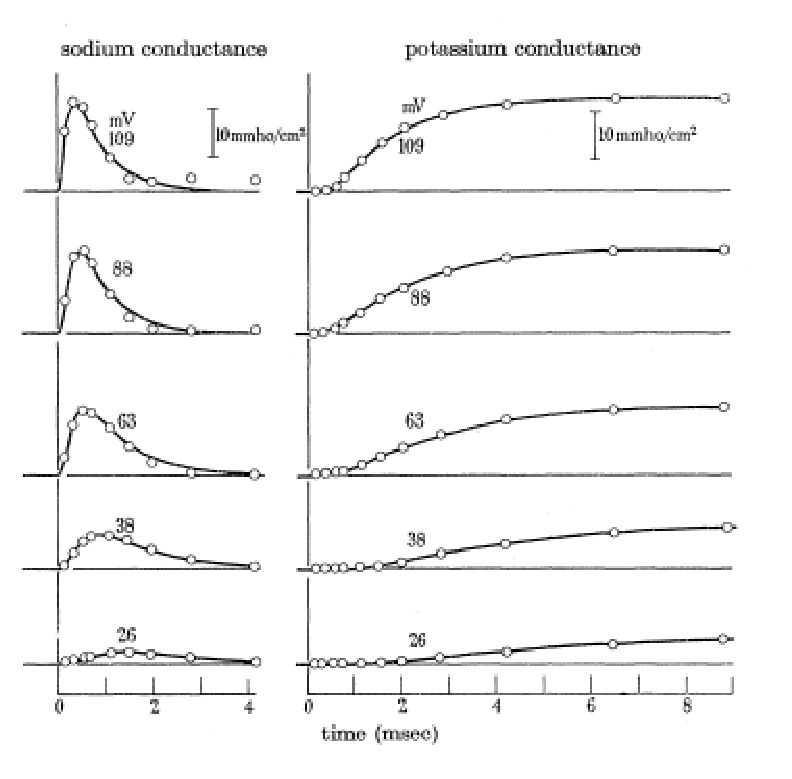
\includegraphics[height=8cm]{./images/sodium-potassium_conductance.eps}}
  \caption{The time course of sodium and potassium conductances
    ($g_{\ce{Na+}}, g_{\ce{K+}}$) at different depolarization
    (mV)~\citep{hodgkin1958cli}. Here Na channels possess a biphasic
    behavior (activation and then inactivation)}
  \label{fig:Sodium-Potassium}
\end{figure}

\subsection{Cable model of axon}
\label{sec:cable-axon}

Given the long axonal fiber, the voltage is not the same everywhere, so there
must be voltage gradient along the fiber, i.e. there exist an axial current.
Modeling voltage propagation is thus an important topic that is discussed in
Hodgkin-Huxley paper. We will go into more details in
Chap.\ref{chap:neuron-models}.



\subsection{Numerical Analysis}
\label{sec:analysis-1}

\subsection{-- Solving integration}
\label{sec:solving-integration}

{\bf In summary}: The Huxley-Hodgkin (HH) model is a set of
4 non-linear ordinary differential equations with time as the
independent variable:
\begin{equation}
  \label{eq:159}
  \begin{split}
    Cdv/dt &= - \overline{g_{\ce{K}}}n^4(v-v_{\ce{K}}) - \overline{g_{\ce{Na}}}
    m^3h(v-v_{\ce{Na}}) - \overline{g_{\leak}} (v-v_{leak}) + I_\app
    \\
    dm/dt &= [-\frac{m-m_\infty(v)}{\tau_m(v)}]\\
    dn/dt &= [-\frac{n-n_\infty(v)}{\tau_n(v)}]\\
    dh/dt &= [-\frac{h-h_\infty(v)}{\tau_h(v)}]\\
  \end{split}
\end{equation}
with $v=V_m-V_r$ is the displacement from the resting potential; the
applied current $I_\app$ can be controlled.

{\bf NOTE}: The small notation $v, v_{Na}, v_{K}, v_{leak}$ represent the
deviation from the membrane resting potential $V_r$, e.g. $v=V_m-V_r$ [mV].
Also, the original paper of Hodgkin-Huxley used the opposite convention. The
value of $V_r$ for the squid giant axon is $-65mV$.  The current density is in
units of $\mu A/cm^2$, conductances in units of $mS/cm^2$, and capacitance is in
units of $\mu F/cm^2$. Also, with
\begin{equation}
  \label{eq:262}
  \begin{split}
    \alpha_n &= \frac{0.01 (10-v)}{\exp(\frac{10-v}{10}) - 1}
    \\
    \beta_n &= 0.125 \exp(-v/80) \\
    \alpha_m &= \frac{0.1(25-v)}{\exp(\frac{25-v}{10})-1} \\
    \beta_m &= 4 \exp(-v/18)\\
    \alpha_h &= 0.07 \exp (-v/20)  \\
    \beta_h &= \frac{1}{\exp\frac{30-v}{10} + 1}
  \end{split}
\end{equation}
The set of these ODEs can be solved numerically (e.g. numerical method of
Hartree, Runge-Kutta method...). \textcolor{blue}{The division by zero occurs at
voltages where the denominator of the rate constant is zero, e.v. $v=10, v=25$. So,
it's important to avoid this or set it to a value closed to zero,
e.g. $v=10.0001, v=25.0001$}.

Using Brunsviga mechanical calculator, it tooks months to solve a few
millisecond of nerve activity~\citep{noble2007}. Thus, it took years to solve
hundreds of milliseconds of cardiac activity.

\subsection{-- Analyze voltage $v$ (or $V_m$)}
\label{sec:analyze-voltage-v}

In order to analyze this model, an XPPAUT script file was created with
given information:
\begin{itemize}
\item $\overline{g}_{Na} = 120$ (mmho/cm$^2$)
\item $\overline{g}_{K} = 36$
\item $\overline{g}_{leak} = 0.3$
\item $V_r = -65$mV (membrane resting potential)
\item $v_{Na} = 115$mV ($E_{Na} = 50$mV)
\item $v_{K} = -12$mV ($E_{K} = -77$mV)
\item $v_{leak} = 10.6$mV ($E_{leak} = -54.4$mV)
\item the specific membrane capacity of squid giant axon is
  $\Csc=1\mu$F/cm$^2$
\item the simulation is performed with an applied current: (1)
  $I_\app=0$, then, (2) $I_\app=6$, (3) $I_\app=7$, (4)
  $I_\app=15$, (5) $I_\app=100$, (6) $I_\app=200$.
\end{itemize}

{\bf NOTE}: Even though the equations were originally based on
experimental voltage-clamp data, the simulation is performed as
current-clamp data (Sect.\ref{sec:current-clamp-protocol}). The reason is that
only with current clamp, we can observe an oscillation. Under the current-clamp case, the equation can
be solved explicitly using numerical methods. Then we can analyze the
data using $V_m-t$ (or $v-t$), $m-t$, $n-t$, and $h-t$ plots.

To solve these 4 ODEs, we need 4 different initial condition values.
\begin{itemize}
\item One for the potential: we have three test cases $V_m(0)=-65,
  -60$, $-58$ mV (equivalent to $v(0)=0,5,7$mV).
\item For $m, n$, and $h$, the steady-state values ($m_\infty,
  n_\infty, h_\infty$) are chosen as initial value to give no
  appreciable error: $m_\infty=0.0529, h_\infty=0.5961,
  n_\infty=0.3176$.
\end{itemize}

\begin{mdframed}
  Runge-Kutta method with time step is chosen as $dt=0.05$ (ms), as
  using the smaller time step 0.01 gives no noticeable change in the
  results.
\end{mdframed}

{\bf XPPAUT code}:\hyperref[HH_model]{Hodgkin-Huxley model}



\begin{figure}[!hbt]
 \centerline{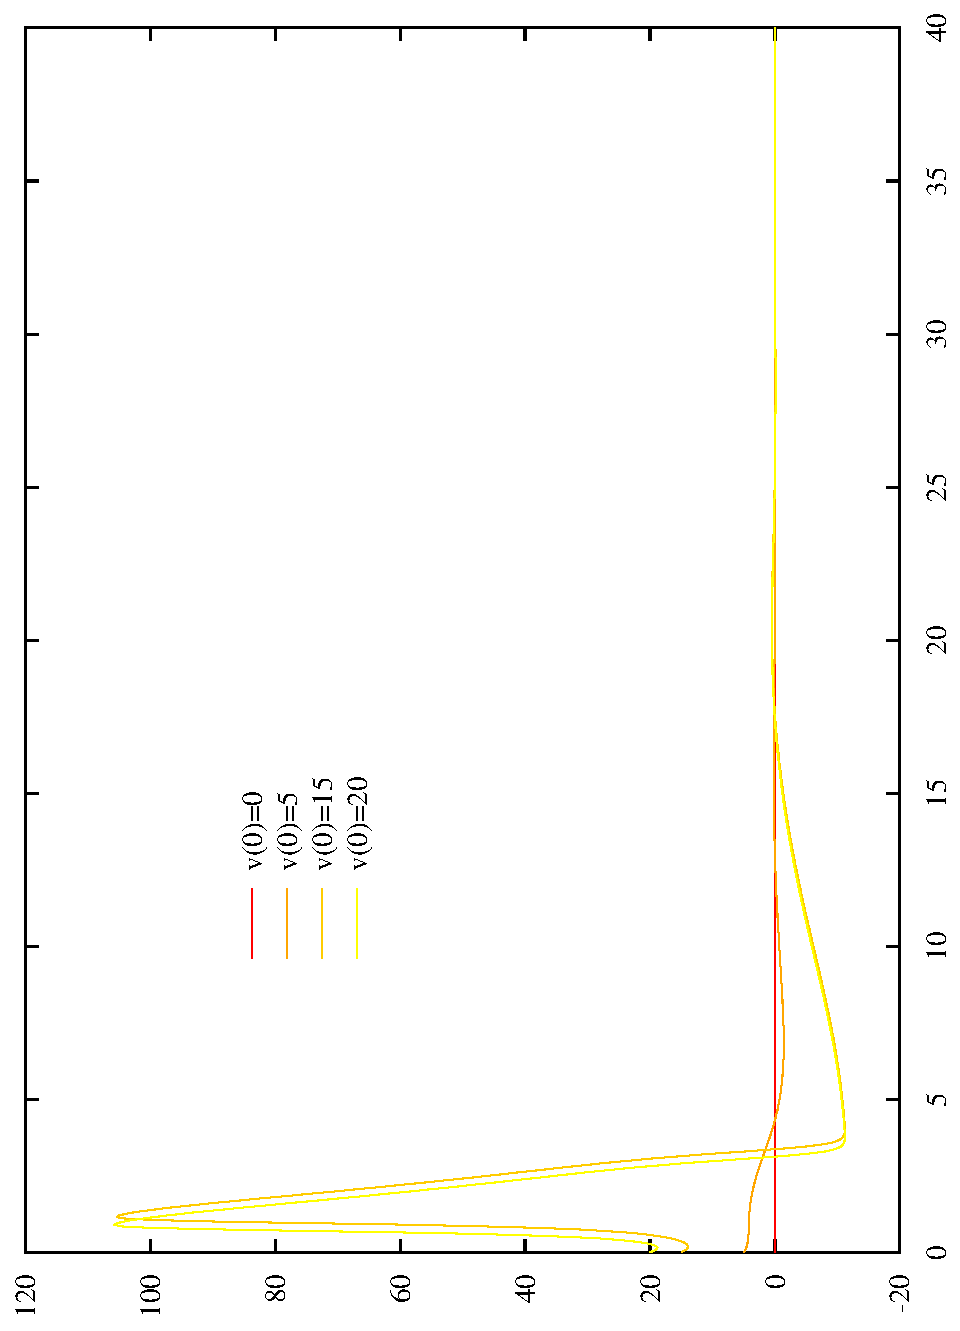
\includegraphics[height=8cm,angle=-90]{./images/HH_model1.eps}}
 \caption{Action potential (AP) $v-t$ plot: the rising of the nerve impulse at
 different initial values of membrane potential $v(0)$ ($I_\app=0$)}
\label{fig:HH1}
\end{figure}



{\bf REMARK}:
\begin{itemize}

\item An  ``all-or-none'' behavior is observed for the AP: when the
  membrane potential passes a threshold, an AP occurs. However, without a
  squared pulse injected current, after returning to the resting state
  value, the membrane cannot fire the AP again, as shown in
  Fig.~\ref{fig:HH1}.

\item The applied current (square wave) play essential role to the
  oscillation of the membrane potential. Simulation result show that
  when $I_\app>7$mA, it causes a continuous spiking (other
  conditions are the same with the previous simulation). However, if
  the applied current is too high, a damped oscillation is observed
  which leads to no electrical propagation or the cell is death, as
  shown in Fig.~\ref{fig:HH2}(b).

  \begin{figure}[!hbt]
    \centerline{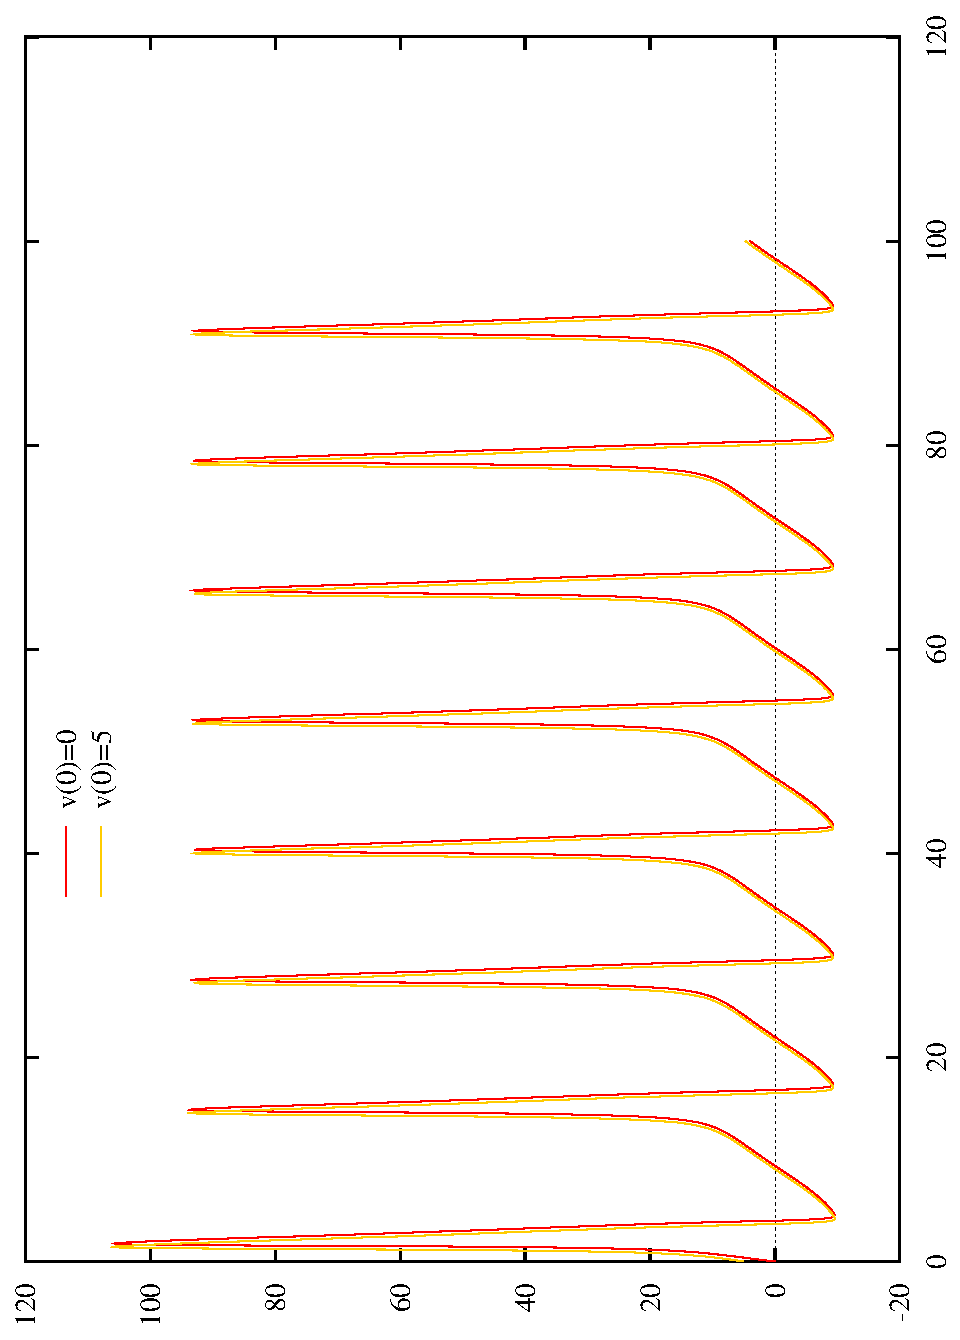
\includegraphics[height=7cm,angle=-90]{./images/HH_model2.eps},
      \includegraphics[height=7cm, angle=-90]{./images/HH_model3.eps}}
    \caption{$v-t$ plot: Continuous spiking (AP in neuron) occurs even when
    the initial values of membrane potential is at rest when there is an applied
      current ($I_\app=15$) and (B) at different values of applied current, and
      v(0)=0. Abscissa: time, Ordinate: voltage}
    \label{fig:HH2}
  \end{figure}

\item Due to the formulation of the gating parameters, when $v(0)=10$
  or $v(0)=25$, the system cannot be integrated as division by zero
  occurs at those equations. Instead, we use an approximate to those
  values for the initial conditions, e.g. $v(0)=10.001$. 

\item Due to the very larges number of ion channels flipping
  stochastically in an all-or-none manner (i.e. from conducting to
  nonconducting states), channels gating appears smooths and graded.


\item $\alpha_m, \alpha_h$ determine the transfer rate from outside
  to inside, $\beta_m, \beta_h$ determine the transfer rate in the
  opposite direction.

\item Since all the parameters are temperature sensitive. Therefore,
  the temperature should be explicitly given whenever the rate is
  recorded.

\end{itemize}



\subsection{-- Analyze $m, n, h$}
\label{sec:analyze-m-n}

Before applying a triggered current, the system should be in a steady
state. Thus, during a simulation, the triggered current is often
applied after a certain amount of time so that the system can reach
the steady state, e.g. for a 1 sec of physiological time simulation,
the current is applied at $t=0.4$ms. However, in this case, the
current is applied from the beginning. So, all initial values should
be chosen as closed to the steady-state values as possible.
\begin{eqnarray}
  \label{eq:579}
  V(0)=V_\infty, m(0)=m_\infty(V(0)), \\
  h(0)=h_\infty(V(0)), n(0)=n_\infty(V(0))
\end{eqnarray}
These steady-state values can be estimated by running the simulation
with $I_\app = 0$ and $V(0)$ is set to the desired steady-state
value. Then, we can find out the appropriate initial values for $m, n,
h$, i.e. $m(0)=0.0529, n(0)=0.3176,h(0)=0.5961$, as shown in
Fig.~\ref{fig:HH_result}.

{\bf NOTE}: If during the simulation, any of the values seem not 
converge to the steady-state value, it means the simulation is not
long enough. There are two ways: (1) run longer, (2) save the last
values, using these values as the initial value and rerun the
simulation.
% The equation for $m, n, h$ can be solved explicitly as they follow
% first-order kinetics, the analytical results are shown in
% eq.~\eqref{eq:61} and eq.~\eqref{eq:66}. The detail has been described
% in the end of each section.

\begin{figure}[hbt]
 \centerline{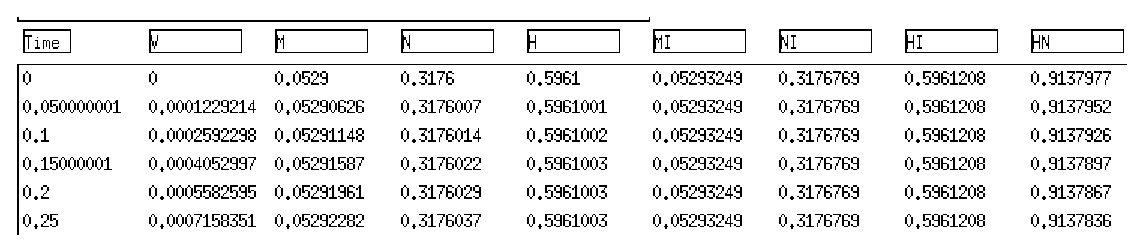
\includegraphics[height=3cm]{./images/XPPAUT_HH_result.eps}}
 \caption{Result for HH model computed with XPPAUT given no applied
   current, $v(0)=0$. The columns are $t,v, m, n,h, m_\infty(v),$
   $n_\infty(v),h_\infty(v),h_\infty(v)+n_\infty(v)$}
\label{fig:HH_result}
\end{figure}

{\bf R-code}: \hyperref[chap2.3.r]{chap2.3.r}


\begin{figure}[hbt]
 \centerline{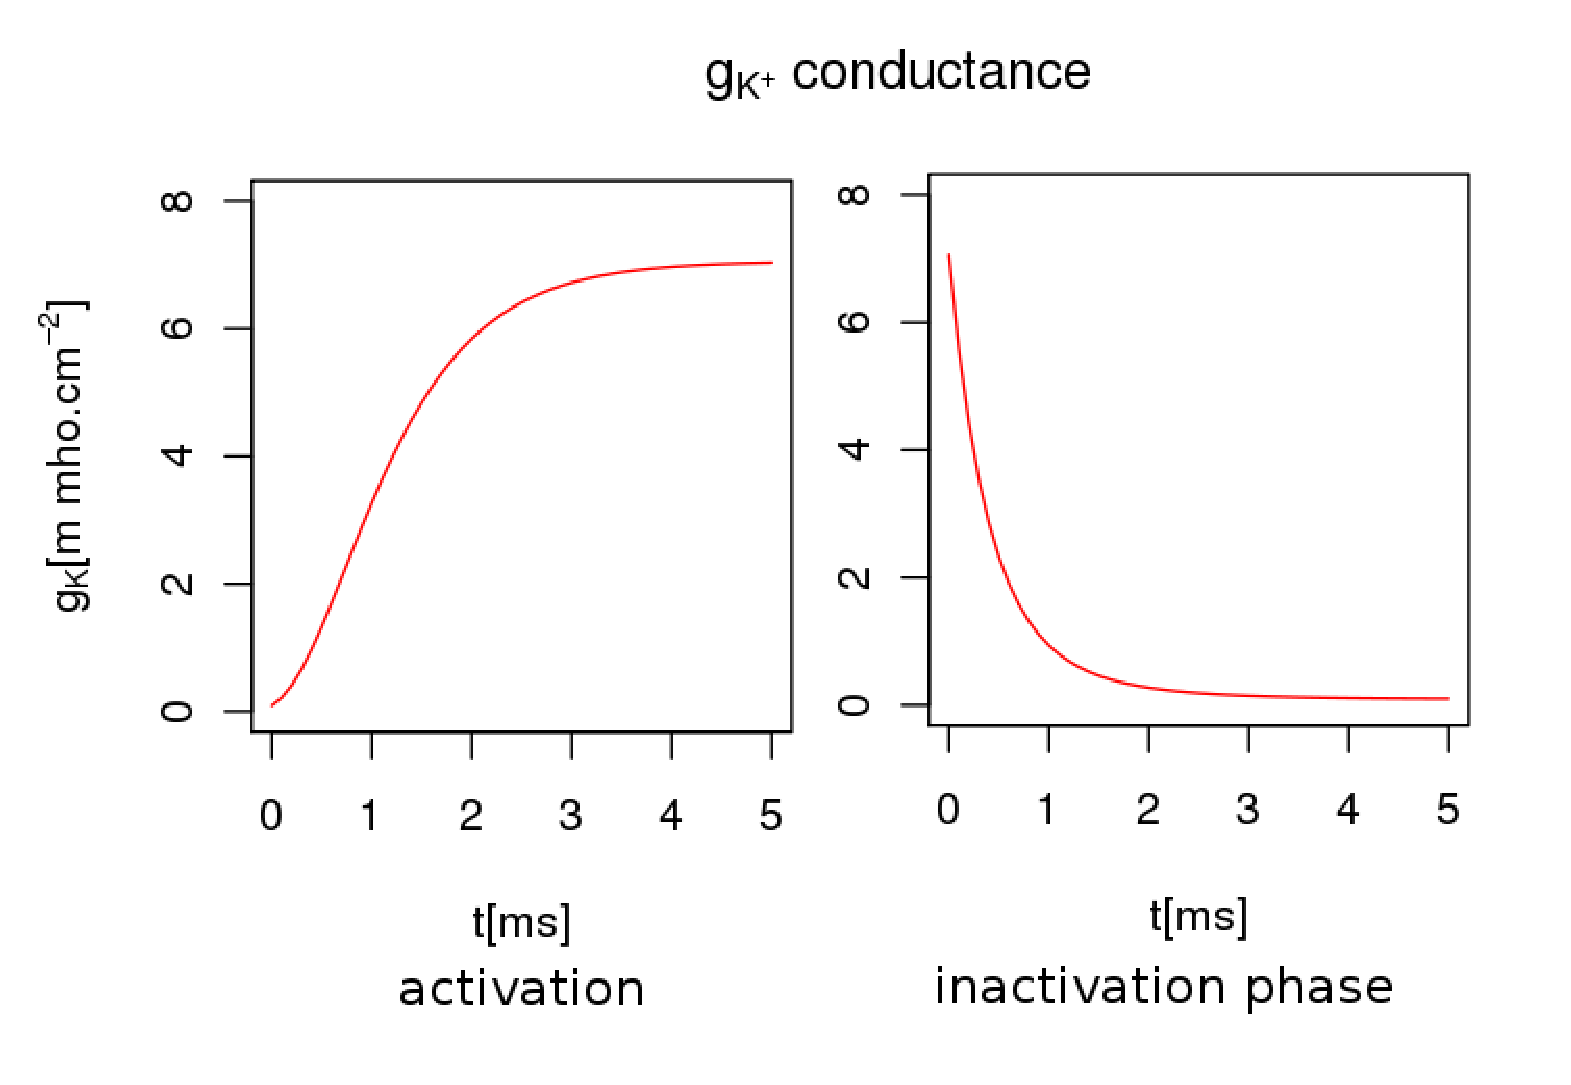
\includegraphics[height=5cm]{./images/K-conductance.eps}}
\caption{Potassium conductance}
\label{fig:K-condutance}
\end{figure}

To plot the falling phase, we invert the values of the $g_{K,\infty}$
and $g_{K,0}$ and the result is shown in Fig.~\ref{fig:K-condutance}.

\subsection{Data analysis}

The equations being used in the model are purely impirical (parameters were
chosen to fit the experimental data). There were no experimental
evidence to support that. However, surprisingly, the model can reproduce many
experimental results. A study to provide a more quantitatively understanding to
the equations being used in the model to provide a guide for making future
modifications to match improved experimental data is discussed by FitzHugh and
colleagues (Sect.\ref{sec:fitzh-nagumo-model}). A typical AP of normal
Hodgkin-Huxley equations is shown in Fig.\ref{fig:FitzHugh1960_Vm}.

\begin{figure}[hbt]
 \centerline{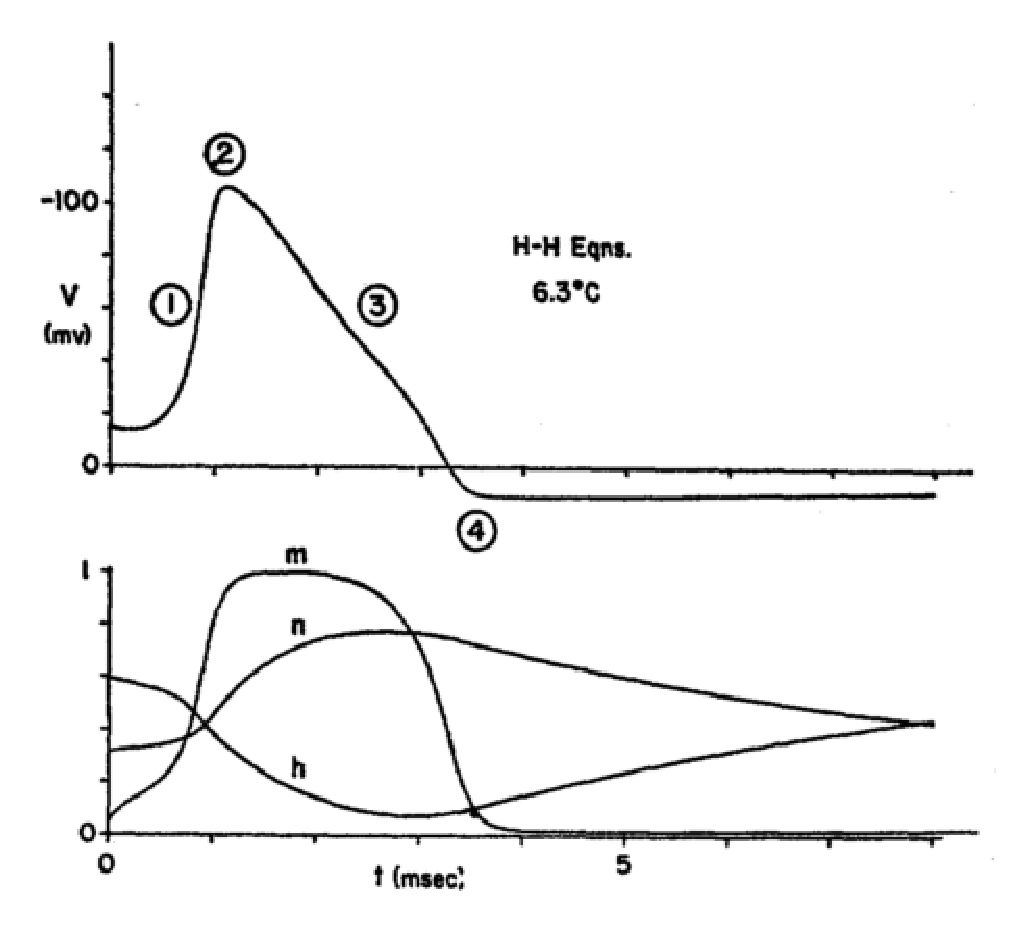
\includegraphics[height=5cm]{./images/FitzHugh1960_Vm.eps}}
\caption{Action potential of a normal Hodgkin-Huxley model}
\label{fig:FitzHugh1960_Vm}
\end{figure}

Although the equations in Hodgkin-Huxley model were developed using
voltage-clamp data; the simulation to test the model was run using current-clamp
conditions. This can reproduce many important physiological properties.


\section{Morris-Lecar model (muscle cell) (1981)}
\label{sec:morris-lecar-model}

In this section, we study one model for muscle cell proposed by Morris
and Lecar~\citep{morris1981vob}. Regardless of the complex voltage
behavior in barnacle fibre, the cell's active conductance were
considered rather simple, with $I_{K}$ and $I_{\ce{Ca}}$ dominating the
membrane and a small leakage current $I_L$. Then, it is reasonable to
assume that the membrane consists of only 2 types of voltage-dependent
channels \ce{Ca^2+} and \ce{K+}. In addition, neither of them
inactivate appreciably.

{\bf NOTE}: In Morris-Lecar model, the effect of calcium-mediated
potassium current \ce{K+_{Ca}} was avoided by using \ce{Ca^2+}
chelator EGTA to reduce its activation.

\begin{figure}[htb]
  \centerline{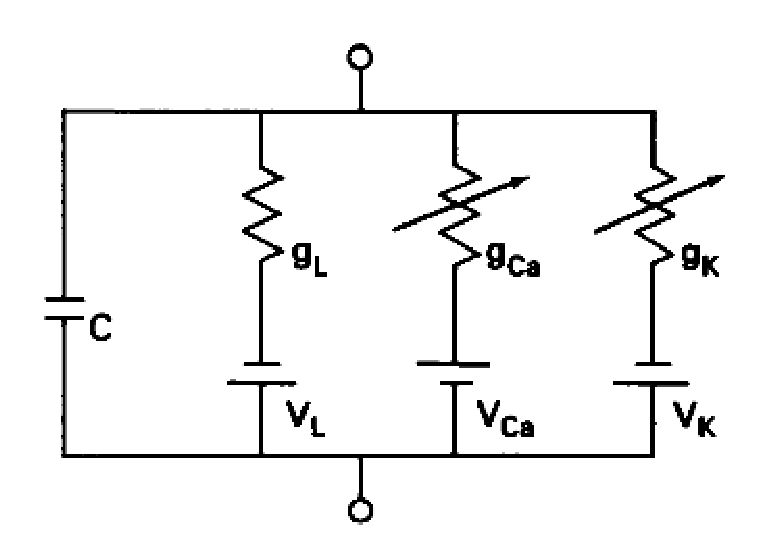
\includegraphics[height=5cm]{./images/barnacle_fiber_circuit.eps}}
  \caption{The equivalent circuit for a patch of space-clamped
    barnacle sarcolema}\label{fig:barnacle_fiber}
\end{figure}

When examining the two types of channels separately, each type of
channels just showed simple shapes potentials while the oscillation
when there are both types of channels is much more complicated
~\citep{morris1981vob}.
\textcolor{green}{The very first assumption is the uniform distribution
  of the ion conductances on the cell, i.e. isopotential of the cell}.
The rising question is that whether those homogeneously distributed
and non-inactivating conductances can create such oscillation?  The
answer was given by Morris and Lacar in their model.  An equivalent
circuit for the barnacle muscle membrane is shown in
Fig.~\ref{fig:barnacle_fiber}.  From that, the dynamic of the membrane
is given in the following general equations


\subsection{Mathematical model}
\label{sec:mathematical-model-6}

In general, the model has a fast activating \ce{Ca^2+} current, a
delayed rectifier \ce{K^+} current and a passive leak. The I-V
equation is given
\begin{equation}
  \label{eq:54}
  \begin{split}
    \Csc\frac{dV}{dt} &= -\overline{g_{\ce{Ca}}} m\times (V-E_{\ce{Ca}}) -
    \overline{g_{\ce{K}}} n \times (V - E_{\ce{K}}) - \overline{g_L} \times(V-E_L) + I_\app \\
    \frac{dm}{dt} &= [m_\infty - m]/\tau_m \\
  \frac{dn}{dt} &= [n_\infty - n]/\tau_n
    % C\frac{dV}{dt} &= -\overline{g_{\ce{Ca}}} f_{\ce{Ca}}\times (V-E_{\ce{Ca}}) -
    % \overline{g_{\ce{K}}} f_{\ce{K}} \times (V -
    % E_{\ce{K}}) - \overline{g_L} \times(V-E_L) + I_\app \\
    % \frac{df_{\ce{Ca}}}{dt} &=
    % [f_{\ce{Ca}_\infty} - f_{\ce{Ca}}]/\tau_{\ce{Ca}}
    % \\
    % \frac{df_{\ce{K}}}{dt} &= [f_{\ce{K}_\infty} - f_{\ce{K}}]/\tau_{\ce{K}}
%   \frac{df_{\ce{Ca}}}{dt} &= k_{\ce{Ca}}(V) [f_{\ce{Ca}}(\infty)-f_{\ce{Ca}}]
%   \\
%   \frac{df_{\ce{K}}}{dt} &= k_{\ce{K}}(V) [f_{\ce{K}}(\infty)-f_{\ce{K}}]
  \end{split}
\end{equation}
with $E_i$ are reversible membrane potential (mV) for channel type
$i$; $\overline{g_i}$ are maximum or instantaneous conductance values
(mho/cm$^2$, m mho/cm$^2$, n mho/cm$^2$),$m,n$ are gating variables
which can be considered as the fraction of open $m_\infty, n_\infty$
are the fraction of open channels at steady state. $V$ is the membrane
potential. $\tau_i(V)$ are relaxation time constants for opening
channels ([ms]).

\begin{mdframed}
  In nerve cells, Na is the inward current. To help bringing the
  activated plasma membrane back to resting potential, an outward
  current carried by K is required. These K channel respond to $V_m$
  in the same way as Na channel does; yet with a slower kinetics. They
  open during the falling phase of AP. For this reason, K channel is
  called {\bf delayed K channels}. Delayed K channels are
  Voltage-gated channels. 
\end{mdframed}
% with $V_i$ are reversible membrane potential (mV) for channel type
% $i$; $\overline{g_i}$ are maximum or instantaneous conductance values
% (mho/cm$^2$, m mho/cm$^2$, n mho/cm$^2$), $f_i$ are the fraction of
% open channels, $f_i(\infty)$ are the fraction of open channels at
% steady state. $V$ is the membrane potential. $k_i(V)$ are rate
% constants for opening channels (s$^{-1}$).
The fraction of open channel $m_\infty,n_\infty$ is a sigmoid function
of voltage $V_m. $ and the (relaxation) time constant $\tau$ is the
bell-shaped function of voltage $V_m$~\citep{lecar1975mcg}. Thus, the
relaxation kinetics is assumed to be first-order. The estimate the
parameters, each type of channels is examined separately.

% \subsection{Analysis}
% \label{sec:analysis-4}

% \begin{equation}
%   \label{eq:48}
%   \begin{split}
%       C\frac{dV}{dt} &= -g_{\ce{Ca}}m_\infty (V-V_{\ce{Ca}}) - g_{\ce{K}} w (V -
%   V_{\ce{K}}) - g_L (V - V_L) + I_\app \\
%   \frac{dw}{dt} &= \frac{\phi(w_\infty - w)}{\tau}
%   \end{split}
% \end{equation}
% with $g_{\ce{Ca}}$ and $g_{\ce{K}}$ are the possible maximum value of the
% conductance of calcium and potassium. $m_\infty$ and $w$ are fraction
% of open channels of calcium and potassium, respectively. $V_i$ is the
% reversible membrane potential.

% The use of $w$ rather the notation $f_0$ is for historical
% reasons. Based on experimental data, they obtained the following
% equations 
% \begin{equation}
%   \label{eq:49}
%   \begin{split}
%       m_\infty &= 0.5 [1 + tanh ((V-v_1))/v_2] \\
%       w_\infty &= 0.5 [1 + tanh ((V-v_3))/v_4] \\
%       \tau &= 1/cosh((V-v_3)/(2.v_4))
%   \end{split}
% \end{equation}
% Why there is no change in $m$? - the fraction of open \ce{Ca} channel
% can be considered a constant in a short enough time constant,
% i.e. $m=m_\infty$.

% Here, we make the assumption without giving argument. We will go into
% detail in Chapter 4 and Appendix A.

\subsection{Data Analysis}
\label{sec:analysis-3}


For a single type of channel $i$, the eq.~\eqref{eq:54} turns into
\begin{equation}
  \label{eq:73}
  \begin{split}
    \Csc\frac{dV}{dt} &= -g_i f \times(V - E_i) - \overline{g_L} \times (V-E_L) + I_\app \\
    \frac{df}{dt} &= \frac{[f_\infty-f]}{\tau}
    % C\frac{dV}{dt} &= -g_i f \times(V - E_i) - \overline{g_L} \times (V-E_L) + I_\app \\
    % \frac{df}{dt} &= \frac{[f_\infty-f]}{\tau}
  \end{split}
\end{equation}
with $f$ can be either $m$ or $n$, and $i$ stands either for \ce{Ca2+}
or \ce{K+}.
\textcolor{red}{It's important to know that $E_{\ce{Ca}} > E_L$ and
  $E_{\ce{K}} < E_L$}.

The dynamic of the reduced system is represented by two differential
equations in~\eqref{eq:73}. Hence, it can be examined using phase
plane analysis, e.g $V, f$-phase plane. The nullclines of the reduced
system is
\begin{equation}
  \label{eq:77}
  \begin{split}
    V(f) &= \frac{g_i f E_i+ \overline{g_L} E_L + I_\app}{g_i f + \overline{g_L}} \\
    f &= f_\infty
  \end{split}
\end{equation}


Applied each type of channels to eq.~\eqref{eq:45}, we have
\begin{equation}
  \label{eq:55}
  \begin{split}
    m_\infty &= 0.5 \left\{1+\tanh(\frac{V-V_1}{V_2})
    \right\} \\
    \tau_m &= \overline{\tau_m}\frac{1}{cosh(\frac{V-V_1}{2V_2})} \\
    n_\infty &= 0.5 \left\{1+\tanh(\frac{V-V_3}{V_4})
    \right\} \\
    \tau_n &= \overline{\tau_n}\frac{1}{cosh(\frac{V-V_3}{2V_4})} \\
    % f_{\ce{Ca}}(\infty) &= 0.5 \left\{ \frac{1}{1+\tanh(\frac{V-V_1}{2S})}
    % \right\} \\
  \end{split}
\end{equation}
When calcium current is examined alone, the I-V is better fit with
\begin{equation}
  \label{eq:617}
  \begin{split}
    I_{Ca} = -{g_{Ca}} .m. R(V,[\ce{Ca^2+}]_i,[\ce{Ca^2+}]_o) \\
    R(V,[\ce{Ca^2+}]_i,[\ce{Ca^2+}]_o) = \frac{V(1-\frac{[\ce{Ca^2+}]_i}{[\ce{Ca^2+}]_o}\exp(\frac{V}{12.5}))}{1-\exp(\frac{V}{12.5})}
  \end{split}
\end{equation}
rather than a linear relation. However, when both \ce{K+} and
\ce{Ca^2+} currents are studied together, the linear approximation is
used. The reason is that the voltage never leaves the non-linear
region. 
% The Morris-Lecar model is the nonlinear model for action potential
% (AP) in the {\it giant barnacle muscle}. This model involves only 2
% free parameters. To study the behavior of ion channels under this
% model, the phase plane technique will be used.

% Experiments have shown that the giant barnacle muscle contains
% primarily voltage gated \ce{K+} and \ce{Ca^2+} currents along with a
% \ce{K+} activated by intracellular \ce{Ca^2+}, a so-called
% \ce{K+_{Ca}} current.



Suppose the cell region's area is $10^{-6}$cm$^{2}$, then the
current's unit is from $\mu A/cm^2$ now to pA.

Let two cases:no applied current, and 
\begin{verbatim}
gL = 2
gK = 8
gCa = 4
V_L = -50
V_Ca = 100
V_K = -70
tau_m_bar = 10
tau_n_bar = 15
V1 = -1
V2 = 15
V3 = 10
V4 = 14.5
Iapp = 50
C = 20
\end{verbatim}

The model produced two modes of oscillations: damped oscillation and
sustained (or limit cycle) oscillation. The barnacle muscle fibre can
produce both types, although it is difficult to distinguish between
them as the damping oscillation is slowly decreased. 

Another parameter set to test:
\begin{verbatim}
gL = 2.0 ; mS/cm^2
gK = 8.0 ; mS/cm^2 
gCa = 4.4 ; mS/cm^2
V_L = 120 ; mV
V_Ca = 120 ; mV
V_K = -84 ; mV
Va = -1.2 ;mV
Vb = 18 ; mV
Vc = 2 ; mV
Vd = 30 ; mV
Iapp = -1 ; uA/cm^2
C = 20 ; uF/cm^2
phi = 0.04 ; temperature adjustment
\end{verbatim}

% \section{Hodgkin-Huxley model and later discoveries}
% \label{sec:discussion-hh-model}


\chapter{Neuron models with Voltage propagation}
\label{chap:neuron-models}

Chap.\ref{chap:point-neuron} focus on modeling a phenomonelogical neuron that
assume isopotential, i.e. single compartment, and consider the neuron as a point
neuron which is simple enough to be used in modeling the interaction of a
network of neurons (Chap.\ref{chap:modeling-network-neurons}).

However, the neuron dendritic tree and axon are quite long such that the
assumption of isopotential is not correct.
Dendrites, but also axon(s), can only be accurately represented as a
multi-compartment model. A few cells can be effectively approximated by two or
three compartments, though a fully accurate model can require very many
compartments.

In this chapter, we discusses how the length of dendrites and axon are
considered in modeling the propagation of membrane potential along the neuron's
branches.

\begin{itemize}
  \item at first, a single branch is assumed, and is modeled as a single
  cylinder.
  
  Sect.\ref{sec:model-an-axon} explains the role of membrane as a capacitor and
  the dynamic resistance of the membrane thanks to the gating of ion channels.
  The propagation of membrane potential is modeled as a hyperbolic PDE
  (Sect.\ref{sec:hyperbolic-pde}).
  Sect.\ref{sec:Hodgkin-Huxley-1952-model-of-propagation} introduced the model in which
  the gating of ion channels using Hodgkin-Huxley-based equations.

  \item as the dendrite of neuron is not a single branch, Rall and collegues
  pionieered in developing a mathematical equation, though for a single
  branch, but incorporate the effect of branching
  (Sect.\ref{sec:non-isop-cell}).
  

  \item 
\end{itemize}

\section{Polarized-cells: Hodgkin-Huxley-based voltage propagation model}
\label{sec:Hodgkin-Huxley-1952-model-of-propagation}
\label{sec:polarized-cell}

% TODO: just extend the cable equation by 
%   using HH-formed of I_\ion

The previous works focus on symmetric cell with uniform membrane potential.
In real cell, they are considered as polarized cells (which has at least basal
and apical dendrites) that may have different potential profiles and non-zero
net fluxes across each. 

The fifth paper in the series (Hodgkin, Huxley (1952), vol. 17) introduced both
the mathematical model for a short-segment of axon of uniform transmembrane
potential. In fact, the complete model of the squid giant axon should be
described using cable equation (Sect.\ref{sec:cable_equation}) which is used to
model the travelling wave of membrane depolarization (more detail, read
Sect.~\ref{sec:non-diment-cable}).

Hodgkin-Huxley derived the mathematical formula for the 2 major ionic currents:
$I_\ion = I_\na + I_\k$ (Sect.\ref{sec:Hodgkin-Huxley-1952-model}). $I_m$ is treated
as the Chlorine-leak current and is part of $I_\ion$.

% In the nerve axon, the propagation of AP along the length of the axon is
% described by the leaky cable. This cable theory was first derived for passive
% membrane, and then for active membrane (Sect.\ref{sec:non-isop-cell}). 

% Sect.\ref{sec:Hodgkin-Huxley-1952-model} explains the mathematical formulas that
% Hodgkin-Huxley used to model the dynamics behavior of the different ionic
% channels, that gives rises to the dynamics of membrane potential.
The equivalent electric circuit for the model of the biomembrane is
given in Fig. \ref{fig:membrane_ionic}. Reminding that the
concentration of \ce{K+} is higher inside and the concentration of
\ce{Na+} and \ce{Cl-} are higher outside. Hence, it's importance to
notice the sign of the reversal potential $V_{K}$, $V_{Na}$,
$V_{Cl}$.

\begin{figure}[htb]
\centerline{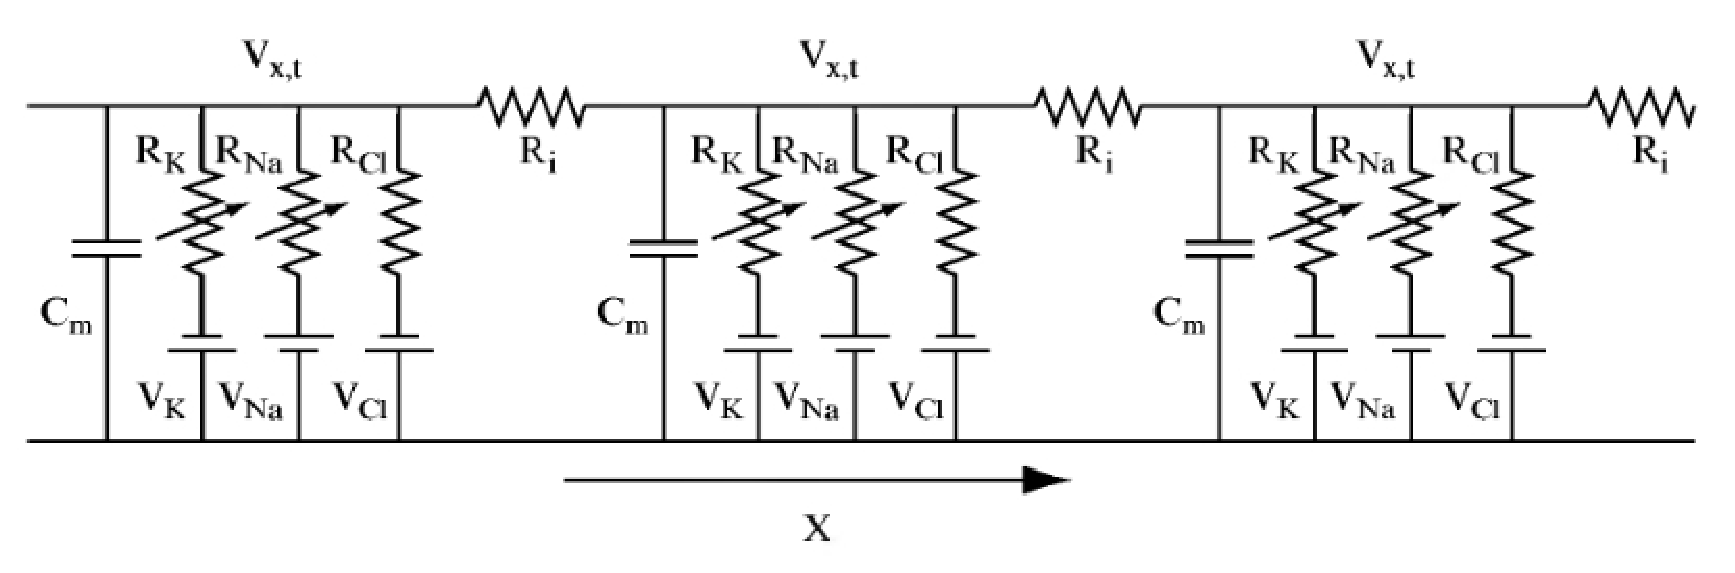
\includegraphics[height=4cm]{./images/membrane_ionic_current.eps}}
\caption{Equivalent circuit of the complex model for the
  membrane}\label{fig:membrane_ionic}
\end{figure} 


% The transmembrane current is
% \begin{equation}
% \label{eq:current-total}
%   I_T = \Cm \frac{\partial V'_{x,t}}{\partial t} + I_{ionic}
% \end{equation}
% The prime in $V'_{x,t}$ (or $V'$ for short) denotes the fact that
% membrane voltage is defined w.r.t the resting potential. 
% The total ionic current is
% \begin{equation}
%   I_{ionic} = I_{Na}+ I_K + I_{Cl}
% \end{equation}
% with the individual component is
% \begin{equation}\begin{split}
%   I_{Na} = g_{Na} (V'_{x,t} - V'_{Na}) \\
%   I_{K} = g_{K} (V'_{x,t} - V'_{K}) \\
%   I_{Cl} = g_{Cl} (V'_{x,t} - V'_{Cl})
% \end{split}
% \end{equation}

% NOTE: We continue to assume that the extracellular resistance is zero,
% $R_0 = 0$. The transmembrane current is equal the gradient of the intracellular 
% current in space
% \begin{equation}
%   i_m = \frac{r}{2\rho_i}\frac{\partial^2V_{x,t}}{\partial x^2}
% \end{equation}
% where $i_m$ is the membrane current density, $r$ is the exon radius
% and $\rho_i$ is the specific resistance of the axoplasm. 
% 
%In summary, from eq.\ref{eq:current-total} we have

From eq.\ref{eq:cable-equation}, we have
\begin{equation}
\begin{split}
  \frac{d}{4 R_i}\frac{\partial^2V_{(x,t)}}{\partial x^2} = & \Csc
  \frac{\partial V_{(x,t)}}{\partial t} \\
   &+ g_{Na,max} m^3h(V'_{x,t} - V'_{Na}) \\
   &+ g_{K,max}n^4 (V'_{x,t} - V'_{K})
  + g_{Cl} (V'_{x,t} - V'_{Cl}) + I_\app
\end{split}
\end{equation}
with $I_\app = \frac{1}{\pi d}I_\inj(x,t)$.

This system contains derivative w.r.t both space and time and thus
it's not easy to solve. However, we can \textcolor{red}{assume} that the
variation of $V_{x,t}$ with time is the same as its variation with location. Then
\begin{equation}
  \frac{\partial^2V_{x,t}}{\partial x^2} = \frac{1}{v^2} \frac{\partial^2V_{x,t}}{\partial t^2} 
\end{equation}
with $v$ being the velocity of conduction of an action potential.

Finally, a single differential equation w.r.t to time is obtained
\begin{equation}
\begin{split}
 \frac{d}{4v^2R_i}\frac{d^2V_{x,t}}{dt^2} = \Csc \frac{dV_{x,t}}{dt} +
 g_{Na,max} m^3h(V'_{x,t} - V'_{Na}) \\
  + g_{K,max}n^4 (V'_{x,t} - V'_{K})
  + g_{Cl} (V'_{x,t} - V'_{Cl})  
\end{split}
\end{equation}
which can be solved numerically if $v$ is known. The approximate value
for the velocity can be obtained from the following formula
\begin{equation}
  v = \sqrt{\zeta.a/2R_i \Csc}
\end{equation}
with $\zeta = 10.47$ ms$^{-1}$ for the squid axon

%\subsection{Propagation of nerve impulses}

A propagating of nerve impulses obeys Hodgkin-Huxley equations
\begin{equation}
\label{eq:cable_HH}
\frac{d}{4R_i}\frac{\partial^2 V_m}{\partial t^2} = \Csc \frac{\partial
V_m}{\partial t} + f(V_m, \ldots)
\end{equation}
with $V_m$ = membrane potential, $a$=radius of axon, $R_i$=resistivity of
axoplasm, $\Csc$=specific membrane capacitance, and $f(V_m,\ldots)$= a
complicated function of $\Vm$ and ionic currents. For the squid's giant axon,
Hodgkin-Huxley reported that $d=480 \mum$, $\rho=0.35 \Omega$.m,
$\Csc=0.01$Farah/m$^2$; and the observed speed of action potential is 21 m/sec.

The myelination around the axon of Schwann cells allow the propagation
of action potential to move forward in a series of jumps. This common
mode of propagation is referred to as {\it saltatory conduction}.

\subsection{-- diffusion constant}

The diffusion constant can be written in the form
\begin{equation}
D = \frac{d}{4R_i \Csc} = 0.034 \text{m}^2/\text{sec}
\end{equation}

In terms of ion, it is discussed in
Sect.\ref{sec:diffusion-particles}.

\subsection{-- mean distance between channels}

The mean distance between adjacent channels of about $0.6\times
10^{-6}$ cm for either type. Based on the intracellular and
extracellular concentration of those ion channels, we have the mean
distance between neighboring ions of about 1.6nm for extra-cellular
sodium and 1.1nm for intracellular potassium. The following table show
the mean distance for all ions, both inside and outside the membrane.

% This LaTeX table template is generated by emacs 22.2.1
\begin{center}
\begin{tabular}{|l|l|l|}
\hline
Inside & Ion & Outside \\
\hline
3.2 &  \ce{Na+} & 1.6 \\
\hline
1.7 & \ce{K+} & 5.5 \\
\hline
2.9 & \ce{Cl-} & 1.4 \\
\hline
\end{tabular}
\end{center}

The next question is {\bf do the ions pass through the hole as
  isolated entities or are they accompanied by some of the water
  molecules?}. - Due to the high charge density of the ions, there is
a first solvation  shell (FSS) of water molecules bound to the ions. In
fact, since sodium is smaller than potassium, and both have the same
charge, the charge density of sodium will higher, i.e. it will attract
more water molecules. In particular, the radius of FSS of the sodium
is 4.9 while that of potassium is 2.9 on average. It seems that some
of the water molecules would indeed accompany each ion, as it passes
through the channel.

% A widely used mathematical formula of this model is Hodgkin-Huxley-based
% equations (Sect.\ref{sec:Hodgkin-Huxley-1952-model-of-propagation})
\section{A single cylinder (cable): model an axon}
\label{sec:model-an-axon}

Due to the wide variation on phenotype of a neuron, the early computational
models of the nerve cells targeted only the axon part of the nerve cell, i.e.
the squid giant axon. 

  % $T=t/\tau_m, X=x/\gamma_m$ are unitless.
  \begin{eqnarray*}
%     \frac{\partial V_m}{\partial T}  =
%     \frac{\partial^2V_m}{\partial X^2} - I_{ion} \Rm
    \Cm \frac{\partial V_m}{\partial t}  =
    \frac{\partial^2V_m}{\partial x^2} - I_{ion} \Rm
  \end{eqnarray*}
  With a steady applied current $I_\app$, the membrane potential would
  equilibrate quickly to
  \begin{equation}
    \label{eq:260}
    V_m = V_{eq} + R_{in} I_\app
  \end{equation}
  However, the eq.~\eqref{eq:260} only holds for small applied
  current. For large current, the response is quite different in
  cells, and thus we need to examine eq.~\eqref{eq:Vm-HH} instead.



We consider only the axon, and perhaps the axon hillock or a single branch of
the dendrite, which can be modeled as a long cylinder of length $x$ with
radius $r$ filled with conducting material in the intracellular medium, the
thickness of the cylinder $h$ is also the thickness of the membrane,
Fig.\ref{fig:membrane-cylinder} (thus called a cable).
\textcolor{red}{The plasma membrane is made of mainly by two layers of
phospholipids molecules - with their  polar heads facing each other - of
thickness $h$} (Sect.\ref{sec:membrane-thickness}).
%one layer is $ \approx 30-50 \AA$}.

Though the cylinder has non-isopotential, this cylindrical piece is divided into
segments of length $\Delta x$, under the assumption that a compartment, a
segment of the cylinder, is isopotential.

\begin{figure}[htb]
\centerline{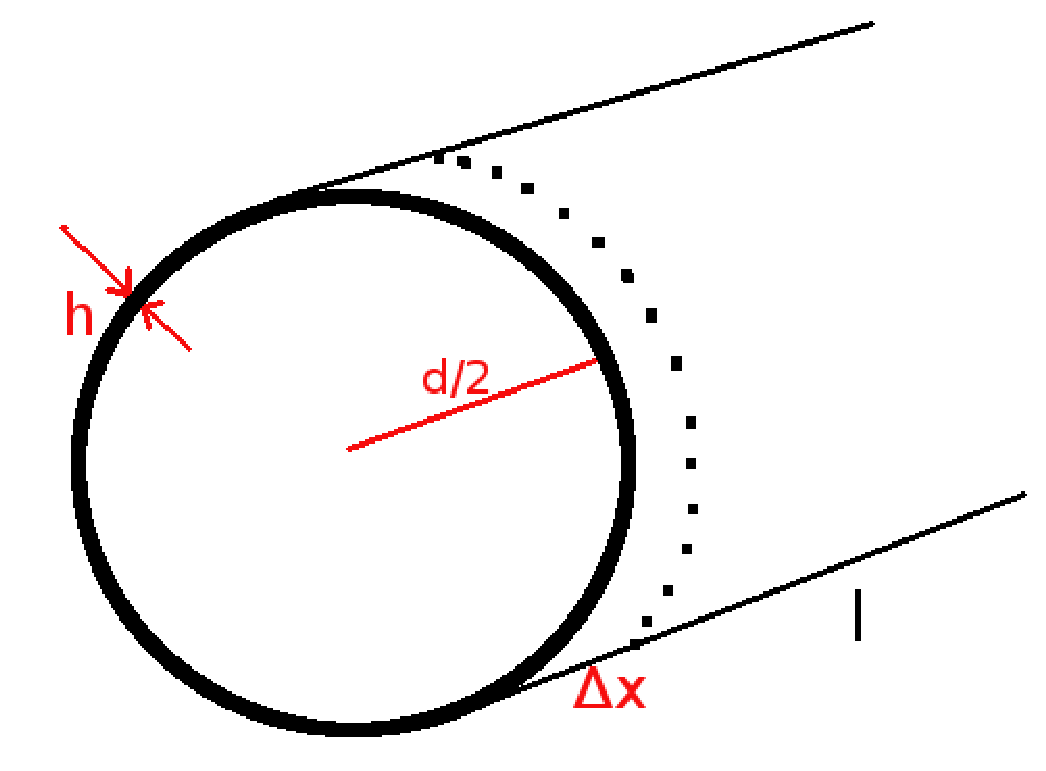
\includegraphics[height=4cm]{./images/membrane-cylinder.eps}}
\caption{An axon with membrane thickness $h$ modeled as a
cylinder of diameter $d$ and length $l$}\label{fig:membrane-cylinder}
\end{figure} 

\begin{enumerate}
  \item The electrical current has 2 components:
  (1) $I_i$ is the current transmitted  along the axon; (2) it may leak through the
  membrane.
  
  As the currents are assumed to flow either horizontally (i.e. along the
cable) or vertically (i.e. across the membrane), the cable can be viewed
as one-dimensional. It is said that ``everywhere along the cable, the potential
depends only on the length variable, and not an radial or angular variables''.
This is known as the {\bf core conductor assumption}.

  \item The resting potential is uniformly distributed along the cylinder.
  
  \item Each cylinder is considered as being immersed in a large volume of
  conducting fluid, i.e. no gradient. The resistance of the fluid (outer
  environment) $R_o$ [Ohm/cm] is thus uniform.
  
  As no extracellular voltage gradient exists, the entire extracellular
  space is isopotential $V_e(x,t) = $constant. Thus, we can safely set it to
  zero; i.e. $R_o = 0$
  
  \item The cytoplasm inside the cylinder, i.e. the {\it axoplasm},
offer a uniform resistance $R_i$ [Ohm per unit length].

  \item We assume that the net resistance across a unit
  length of the membrane thickness is $R_m$ [Ohm per unit length] (fixed value).
\end{enumerate}

In Sect.\ref{sec:simple-model-passive}, we treat the membrane as simple as a
resistor with constant resitance (R) where the membrane potential passively
propagate along the cylinder. However, this does not explain the slow decay of
qthe membrane potential. This requires a new information
(Sect.\ref{sec:moder-model-active})

\begin{enumerate}
  \item [6.] The plasma membrane functions as a capacitor with capacitance C
  [Coulomb] that separate the ions on each side of the membrane.  
\end{enumerate}
This explains the slow decay, but still not enough to explain the fast
propagation of the membrane potential, under neuron's spike generation. 
This requires a new information (Sect.\ref{sec:complex-model-action})
\begin{enumerate}
  \item [7.] On the plasma membrane, there exists proteins that gates the
  transportation of ions across the membrane, so that once the gates open, it
  quickly reduces the resistance to enable the fast propagation of membrane
  potential $V_m$.
\end{enumerate}

% To study the electrochemical properties of nerve cells, we have to
% develop a good model of them with the following assumptions.
%. Every model still requires some assumptions:

%\subsection{Cable model of a cylindrical axon}
\subsection{Simple model - passive process}
\label{sec:simple-model-passive}

First, we want to examine the spatial gradient of the electrical potential
without ion channels and the ions on each side of the membrane. So, we can
ignore the effect of the capacitor C. Under such assumptions, we have the
equivalent circuit for such cylinder as shown in \ref{fig:circuit1}.

\begin{figure}[htb]
\centerline{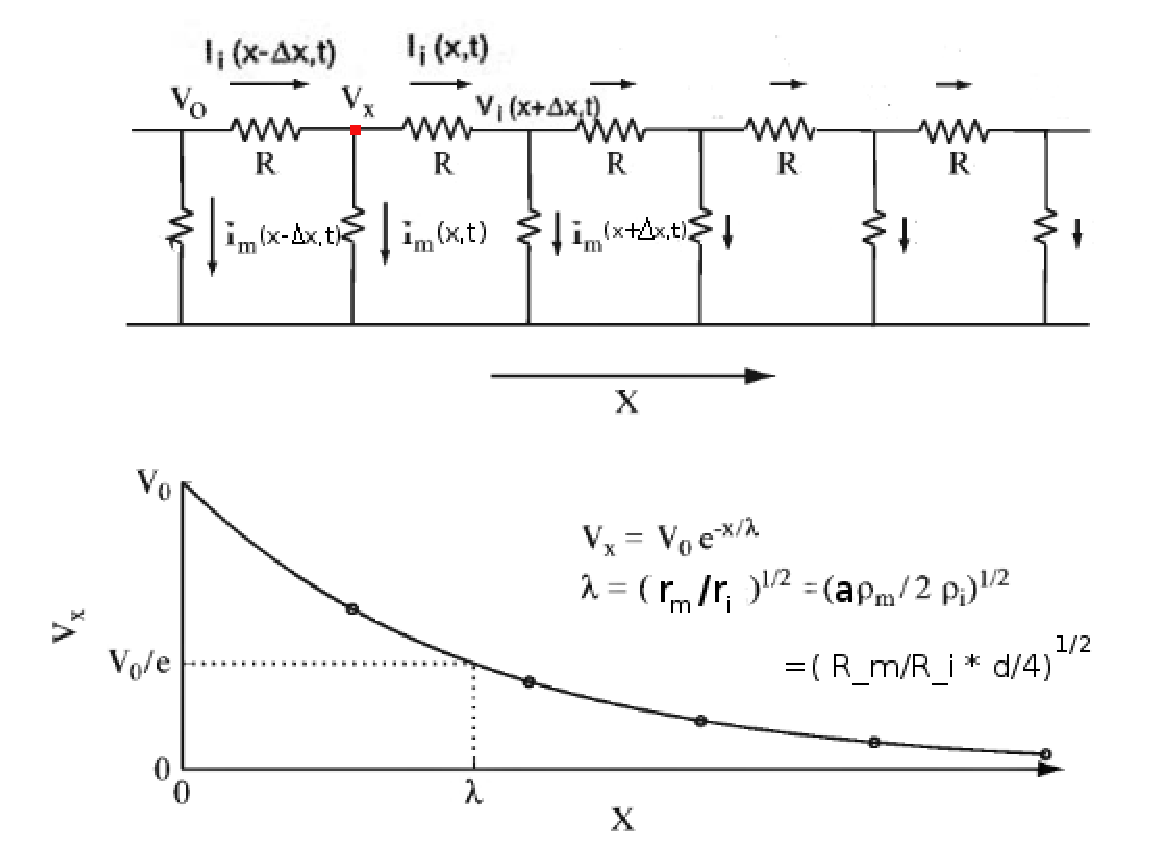
\includegraphics[height=7cm]{./images/membrane_simplemodel.eps}}
\caption{A passive nerve process $R_0 = 0$: the current flows in 2 directions:
axial direction with intracellular resistance is modeled by the purely ohmic
resistance $R$ (Ohm), and cross-membrane direction is represented as $i_m(x,t)$.
The diameter of the cable $d=2\times a$, the membrane resistivity $\rho_m$ and
intracellular resistivity $\rho_i$. The membrane potential decay exponentially,
with the speed of the decay is represented by the length constant $\lambda$
which is a function of membrane resistance property $r_m$ and intracellular
medium's resistance per unit length $r_i$}\label{fig:circuit1}
\end{figure} 

Let's examine a segment of isopotential membrane $l=1$(unit), as shown in
Fig.~\ref{fig:circuit1}. In any cable section, the currents must balanced,
with only two types of currents: transmembrane current ($I_m$) and axial
current ($I_i$ and $I_e$).
% \begin{eqnarray}
%   \label{eq:489}
%   r_i &=& \frac{4R_i}{\pi d^2} \\
%   r_m &=& R_m/(\pi d)
% \end{eqnarray}
% with $R_m$(Ohm.cm$^2$) resistance across a unit area of membrane,
% $R_i$(Ohm.cm) specific resistance of the internal medium.
% 

There are two axial currents: intracellular $I_i$ and extracellular $I_e$
components. Under electrotonus condition
(Sect.\ref{sec:electrotonus_vs_transient}), both currents are assumed to be
linear functions of the voltage.

\begin{equation}
  \label{eq:421}
  \begin{split}
    V_i(x+dx)-V_i(x) &= -R \times I_i(x)\\
    V_e(x+dx)-V_e(x) &= -R_e \times I_e(x)
  \end{split}
\end{equation}
with R (Ohm), $R_e$ (Ohm), $I_i(x), I_e(x)$ (A).
% with $r_i, r_e$ are resistances of
% the intracellular and extracellular media, respectively, and are in unit of
% resistance per unit length (Ohm/cm or Ohm/mm).
The minus sign appears on the right-hand size because of the convention that
positive current is the flow of positive charges from the left to the right
(i.e. in the direction of increasing $x$).

In the limit of an infinitestimal small interval $dx \rightarrow 0$,
\begin{equation}
  \label{eq:422}
  \begin{split}
    I_i &= -\frac{1}{r_i}\frac{d V_i}{d x} \\
    I_e &= -\frac{1}{r_e}\frac{d V_e}{d x} 
  \end{split}
\end{equation}
with $r_i = R/\Delta x$ is intracellular resistance per unit length of cable
[Ohm/cm]

NOTE: \textcolor{red}{Here, the voltage is only the function of distance}
$V_i(x)$, 
% By using the Ohm law for the axial current:
% $  I_i(x) = \frac{V_i(x) - V_i(x+\Delta x,t)}{R_i^0} $, then
% \begin{equation}
%   \label{eq:Ohm-law}
%  -I_i(x) = \frac{d  V_i(x)}{R_i^0} =  \frac{d  V_i}{R_i\times
%  d x}
% \end{equation} 
with $d  V_i = V_{i,1}-V_{i,2}$ is 
the difference potential between two
ends of the small segment of the cylinder at a distance $\Delta x$ 
(NOTE: $V_1$ is near the starting end). 

As we assume there are only two types of currents, intracellular
current and transmembrane current, using Kirchoff law which states that the sum
of all currents flowing into and out of any node must equal zero.
\begin{equation}
i_m(x,t) + I_i(x,t) - I (x-\Delta x, t) = 0
\end{equation}
and in differential form ($\Delta x \rightarrow 0$)
\begin{equation}
  \label{eq:43}
  i_m(x,t) = I_m =   -\frac{dI_i}{dx} 
\end{equation}

We take a derivative of eq. \ref{eq:422} to get the right-hand side of
eq.\ref{eq:43}.

% We can write eq.~\eqref{eq:Ohm-law} in
% the form of derivative
% \begin{equation}
%   -I_i = \frac{1}{R_i} \times \frac{d V}{d x}
% \end{equation} 
% or 
\begin{equation}
  \label{eq:dIidx}
  -\frac{dI_i}{dx} =  \frac{1}{r_i} \frac{d^2 V_i(x)}{d x^2}
\end{equation} 

% As we assume there are only two types of currents, intracellular
% current and transmembrane current, using Kirchoff law, the loss in the axial
% current should be the transmembrane current $I_m$.
% In other words, we have
% \begin{equation}
%   \label{eq:43}
%   -\frac{dI_i}{dx} = I_m
% \end{equation}

\begin{mdframed}

In this case: in addition to the resistance of the membrane $R_m$, we also have
the resistance of the cytoplasm $R_i$ and the extracellular space $R_o$. For the
sake of simplicity, the extracellular is assumed to be isopotential, i.e. no
resistance $R_e=R_o=0$ in most of the cases. This is based on the assumption
that the extracellular space is either a perfect conductor or of infinite
extent.
However, in some special problems, e.g. the tightly packed axons in a nerve
trunk or for neurons in a CNS where the current flow in the extracellular may be
significant, $R_o$ may be non-zero.
\end{mdframed}

Consider $V_m = V_i - V_o$ is the transmembrane potential, so,
\begin{equation}
  \label{eq:126}
%  I_m =  \frac{V_m}{R_m^'} = \frac{V_m}{R_m .h}
  i_m =  \frac{V_m}{r_m}
\end{equation}
% with $R_m'=R_m^0\times h$ [Ohm.m].
% with [$I_m$] = [A/m], [$R^0_m$]=[Ohm].


NOTE: As $V_e(x)= const$, 
$\Delta V = V_1-V_2 = (V_1 - V_{out}) - (V_2 -V_{out}) = V_{m,1} = V_{m,2} =$
$\Delta Vm$, or $d V = d V_m$.
Combine this with eq.\ref{eq:126} and eq.\ref{eq:43} and eq.\ref{eq:dIidx}:
\begin{equation}
  \label{eq:127}
  V_m = \frac{r_m}{r_i} \frac{d ^2V_m}{d x^2}
\end{equation}

\begin{mdframed}[linecolor=red!60!black,  linewidth=2pt]
In the simple case, we assume the outside medium has 
$R_{0} = 0$, so $V_{out}= 0$ or $V_m = V_x$. 
The general solution of ~\eqref{eq:127} is
\begin{equation}
  V_x = A.\exp \left( \frac{-x}{\sqrt{r_m/r_i}} \right) +  B.\exp
  \left( \frac{x}{\sqrt{r_m/r_i}} \right)
\end{equation}

% TODO: find the meaning of B in second term ?

{\bf What are the values of A, B?}: In a passive cable, since $V_x$ tends to
zero when $x\rightarrow \infty$, so we can eliminate the second term,
i.e. $B=0$.
\begin{equation}
   V_x = A.\exp \left( \frac{-x}{\sqrt{r_m/r_i}} \right) 
\end{equation}

\end{mdframed}

Assuming that at one end of the axonal process, the initial potential
is $V_x = V_0$, at $x=0$. Then, $A = V_0$ or
\begin{equation}
  \label{eq:128}   V_x = V_0.\exp \left( \frac{-x}{\sqrt{r_m/r_i}} \right) 
\end{equation}
The term in the exponent should be unitless. This is true since
[$r_m$]=[Ohm.cm] while [$r_i$]=[Ohm/cm], using \eqref{eq:resistance},
we have
\begin{equation}
  \sqrt{r_m/r_i} = \sqrt{\frac{\rho_m\Delta
      x h}{2\pi.r.h}/\frac{\rho_i}{\pi.r^2}} = \sqrt{r\rho_m\Delta x/2\rho_i}
\end{equation}
So, the thickness of the membrane is canceled out, and is thus not play a role
to the decay of the voltage. Next, we define:
\begin{equation}\label{eq:rhom}
  \rho_m' = \rho_m. \Delta x
\end{equation}
with $\rho_m$ is the resistivity of the membrane so that we can use it
to compute $r_m$.


\subsection{-- membrane thickness (h)}
\label{sec:membrane-thickness}

Each layer of membrane phospholipid bilayer is $ \approx 30-50 \AA$, and the 
lipid bilayer is about 6-10 nm. 

In the axon, we need to use a different value for $h$, which is quite large due
to the myelinated sheath. The usual thickness of the myelin sheath is between
200 and 800 $\mum$.

Myelin increases resistance across the cell membrane by a factor of 5,000 and
decreases capacitance by a factor of 50 (Sect.\ref{sec:myelin-sheath}).



\subsection{-- length constant of a cable ($\lambda$)}

The denominator in the exponential term of eq.~\eqref{eq:128} is called the
{\bf length constant} (in unit of distance), denoted by $\lambda$ (lambda), as
it is the distance from that the membrane potential decrease (1/e)
\begin{equation}
  \lambda = \sqrt{r_m/r_i} = \sqrt{r\rho_m'/2\rho_i}
\end{equation}
with $\rho_i$ is unit of resistance times {\it length}, $\rho_m'$ is
unit of resistance times {\it area}. {\bf The length constant is the
distance at which the transmitted signal drop 1/e (or about 63.2\%) of
its initial magnitude.}

{\bf Example:}: A bare crustacean (gia'p xa'c) has its axon with a diameter
$d=30\mu m$ and typically has the resistivity $\rho_m' = 5000$Ohm.cm$^2$, and
$\rho_i = 50$Ohm.cm which gives a length constant $\lambda \approx 2.7$mm. The
given length constant tells us that the initial electrical potential decrease a
factor of (1/e) after a distance of 2.7mm. This is too short and a disadvantage
for long distance transmission of signal, e.g. from brain to the foot. To
transmit about 1 metre in length, an axon should have a diameter of about 5m.
This is clearly not a practical proposition.

In such sense, the length constant of 2.7mm may be enough for handling
the signal that pass along the dendrites (i.e.
{\it passive cable response}) and impinge upon the soma. So, it is
acceptable to model the dendrites using this model.  A conclusion is
withdrawn: {\it To have a good model for the axon's signal transmission, we
should take into account the influences of the membrane capacitance C}
(Sect.\ref{sec:moder-model-active}).

\subsection{Moderate model - membrane as capacitor}
\label{sec:moder-model-active}

The electrical signal cannot propogate that far in a passive model
(Sect.\ref{sec:simple-model-passive}) due to the strong leak current. For the
nerve cell to propagate the signal far enough, the membrane should serve as
an insulator to prevent this leak.
Whenever there is an insular keeping charges apart; it will act like a capacitor
with a given capacitance C (Sect.\ref{sec:capacitance-in-neurons}). A standardized
measurement, called as {\bf specific membrane capacitance} called $\Csc$ is often used
(Sect.\ref{sec:specific-membrane-capacitance}).
As a result, the equivalent electric circuit for a cylinder is
shown in Fig.~\ref{fig:cylinder}. 

% \begin{figure}[hbt]
%   \centerline{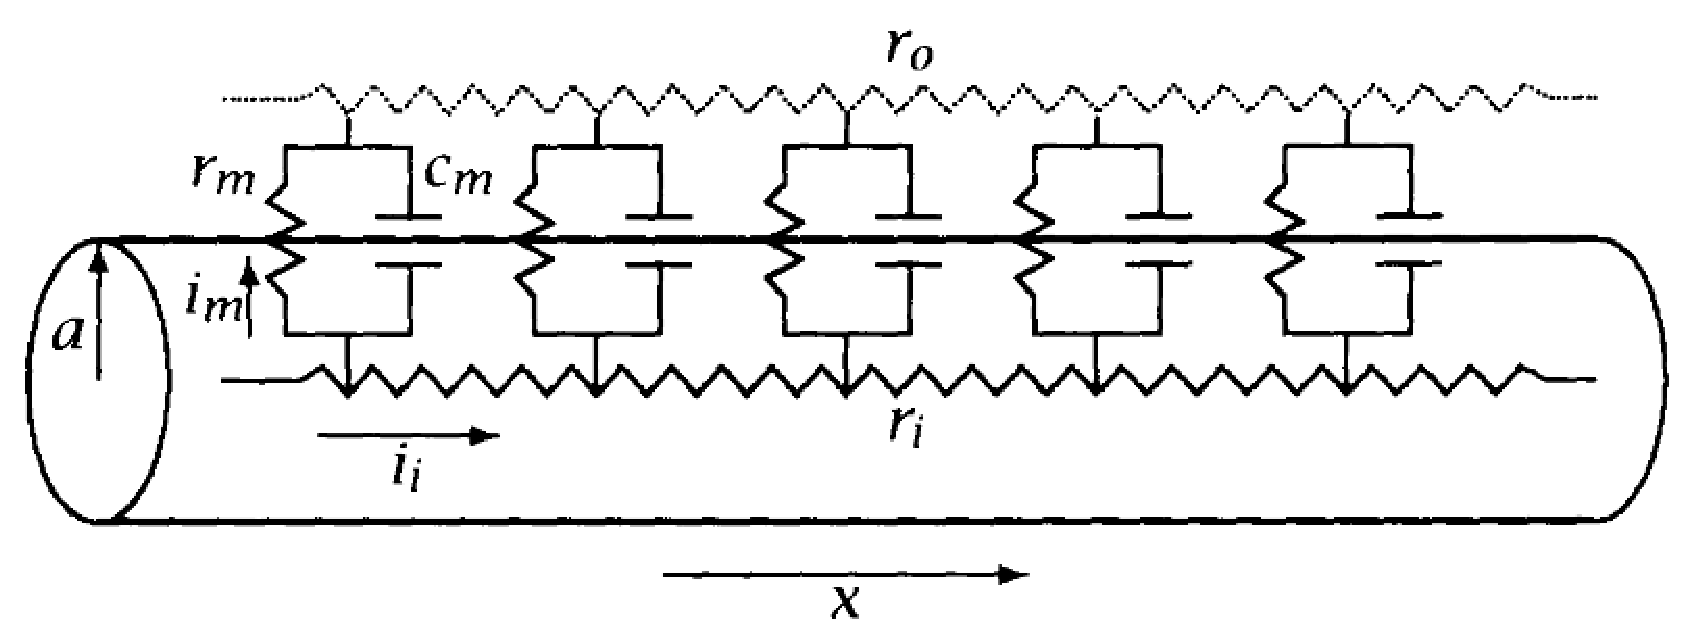
\includegraphics[height=4cm,
%     angle=0]{./images/cylinder_cell.eps}}
% \caption{A cylinder with multiple compartments}
% \label{fig:cylinder}
% \end{figure}

% \begin{figure}[htb]
% \centerline{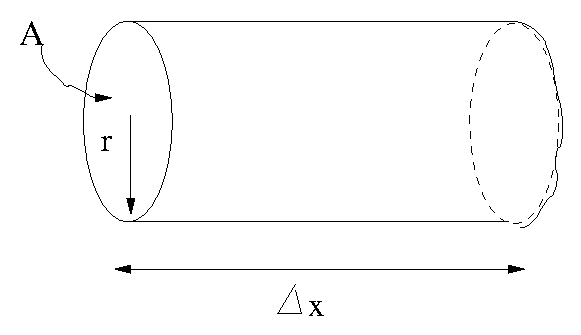
\includegraphics[height=4cm]{./images/cylinder.eps}}
% \centerline{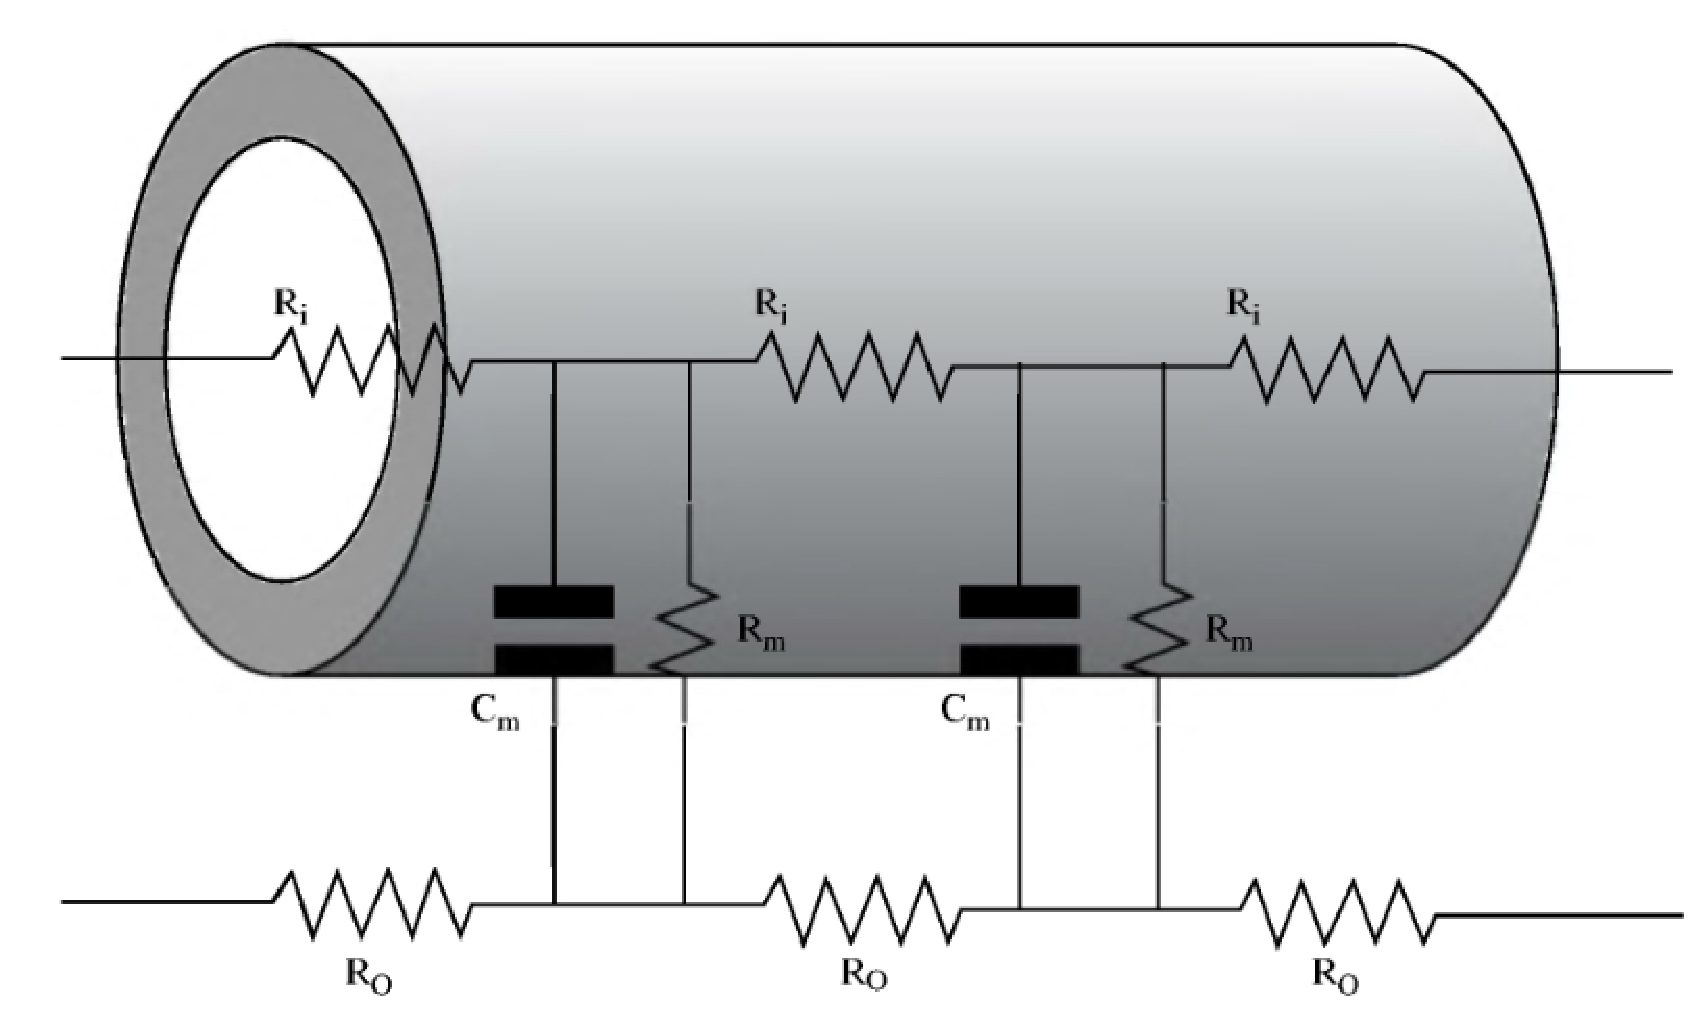
\includegraphics[height=4cm]{./images/nerve-process.eps}}
% \caption{A nerve process (axon or dendrite)}\label{fig:cylinder}
% \end{figure} 

\begin{figure}[htb]
\centerline{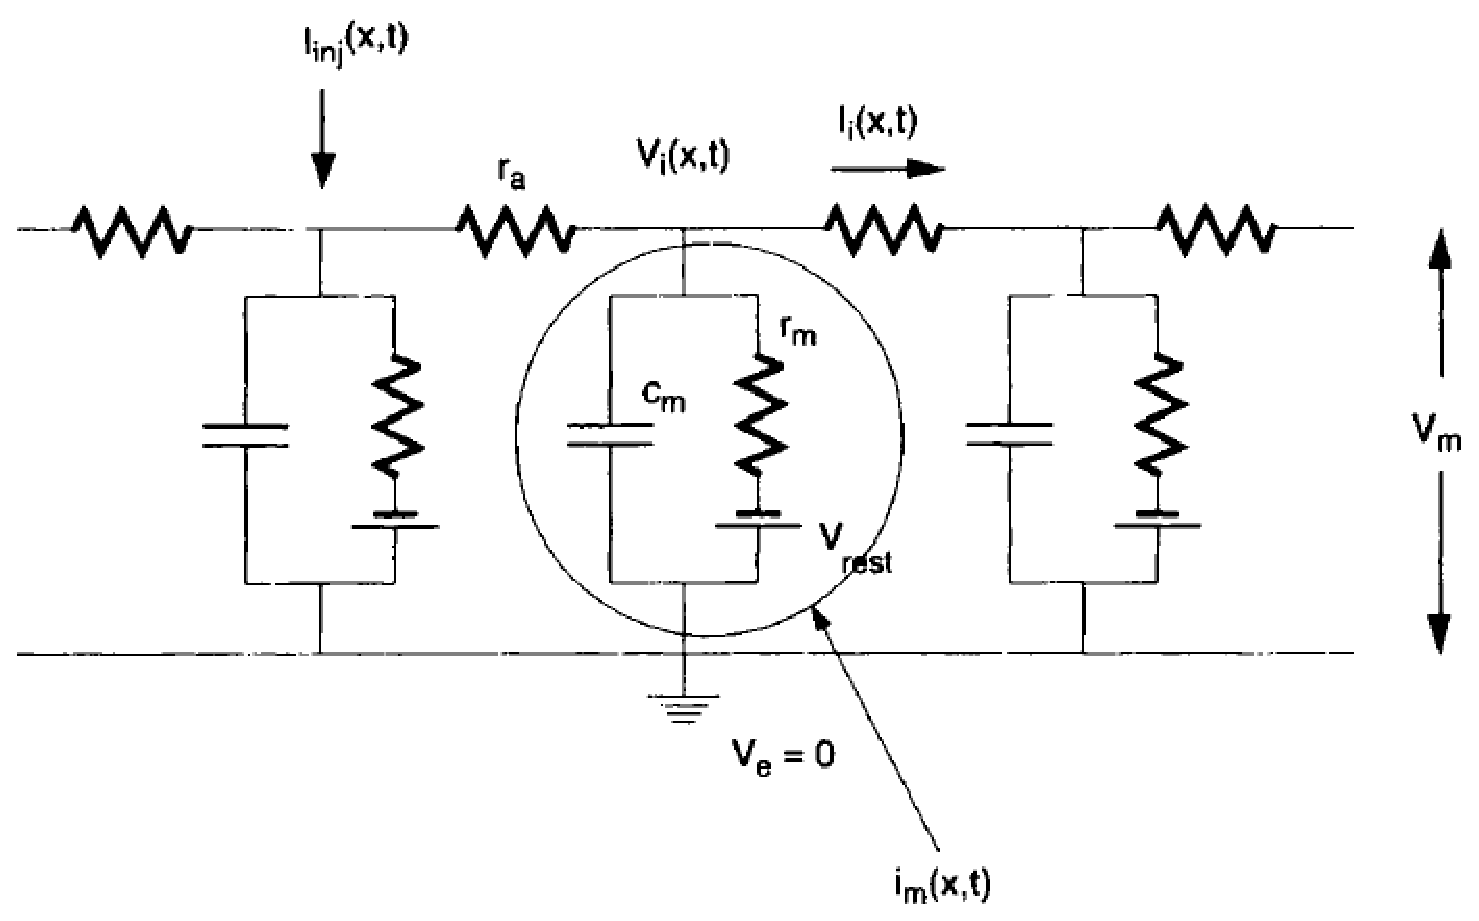
\includegraphics[height=4cm]{./images/membrane_RC-model.eps}}
\caption{A nerve process (axon or dendrite) with an
external current $I_{inj}(x,t)$ is injected into the cable}\label{fig:cylinder}
\end{figure} 

With the presence of a capacitor, the longitudinal current $I_i$ and the voltage
$V_i$ are now both distance-dependent and time-dependent, i.e.  we now replace
$I_i$ and $V_i$ by $I_i(x,t)$ and $V_i(x,t)$, respectively. 

Under the assumption of $R_o = 0$ (i.e. $V_o(x,t) = const$), then $V_i(x,t)$
becomes $V_m(x,t)$. Eq.\ref{eq:dIidx} becomes
\begin{equation}
  \label{eq:dIidx_capacitor}
  -\frac{\partial I_i(x,t)}{\partial x} =  \frac{1}{r_i}\frac{\partial
  ^2V_m(x,t)}{\partial x^2}
\end{equation} 

% 
% Similarly, we have
% \begin{equation}
% -I = \frac{1}{R_i} \frac{\partial V}{\partial x} 
% \end{equation}
% Under the assumption of $R_o = 0$ (i.e. $V_o(x,t) = const$), then
% \begin{equation}
% \label{eq:Ileak_2}
% -I = \frac{1}{R_i} \frac{\partial V_m}{\partial x}
% \end{equation}

The current can now leak through not only the
resistance $r_m$, but also the capacitor.  The leakage
current should have an additional term (and in general a third term is added as well)
\begin{equation}
\label{eq:dIidx_active}
%  \Delta I = -\frac{dI}{dx}= \frac{V}{R_m'} + \Cm \frac{dV}{dt}
-\frac{\partial I_i(x,t)}{\partial x} = \underbrace{\frac{V_m(x,t)}{r_m}}_{I_m}
+ \underbrace{c_m
\frac{\partial V_m(x,t)}{\partial t}}_{I_c} - I_\inj(x,t)
\end{equation}
with the second term on the right side is the current leakage through the
capacitor, i.e. {\it capacitive current}
$I_c$ (Sect.\ref{sec:capacitive-current}); and the third-term is current
injection.

Combine eq.\ref{eq:dIidx_capacitor} with eq.\ref{eq:dIidx_active}, we
have
\begin{equation}
  \label{eq:129}
  \frac{1}{r_i} \frac{\partial ^2V_m}{\partial x^2} = 
  \frac{V_m}{r_m} + c_m
  \frac{\partial V_m}{\partial t} - I_\inj
\end{equation}
% or
% \begin{equation}
%   \lambda^2 \frac{\partial ^2V_m}{\partial x^2} = V_m + \tau
%   \frac{\partial V_m}{\partial t} - I_\inj
% \end{equation}
which is a hyperbolic PDE (Sect.\ref{sec:hyperbolic-pde}).

\begin{mdframed}[linecolor=red!60!black,  linewidth=2pt]
In this model, we keep assuming the resistance of
the extracellular fluid is zero, $R_0 = 0$.
The general solution of eq.~\eqref{eq:129} is
\begin{equation}\label{eq:Vxt}
\begin{split}
  V &= V(x,t) \\ 
   &= \frac{V_0}{2}\left( e^{-x/\lambda}
    \text{erfc}(\frac{x/\lambda}{2\sqrt{t/\tau}}-\sqrt{t/\tau}) + e^{x/\lambda} \text{erfc}(\frac{x/\lambda}{2\sqrt{t/\tau}}+\sqrt{t/\tau}) \right)
\end{split}
\end{equation}
with $\lambda = \sqrt{r_m/r_i}$ is the length constant and 
$\tau =r_mc_m$ is the {\it time constant}. The time constant is the
  duration of time required for the stimulus to increase the potential
  e times (62.3\%) of the original value. The symbol {\it erfc} denotes the
complementary error function, it means

\begin{equation}
  \label{eq:130}
     \text{erfc(k)}= 1 -
  \frac{2}{\pi}
  \int_0^{k} e^{-y^2} dy
  \\
\end{equation}

\end{mdframed}

\subsection{-- capacitance in neuron}
\label{sec:capacitance-in-neurons}

Capacitance is a fundamental neuronal property. 
Sect.\ref{sec:capacitance} discusses  different methods to estimate capacitance.
\citep{golowasch2009} showed that these methods result to significantly
different values; and they suggested that
\begin{enumerate}
  \item  current-clamp method is a good choice for cells even with complex
  architecture. other methods (voltage-clamp step or ramp protocols) yield
  significant errors for neurons whose membrane structure is not electrotonically compact.

With highly complex neurons the current-clamp step method still can
underestimate the capacitance due to numerical errors introduced by
multiexponential fitting methods.

   \item When measurements are done with both current- and voltage-clamp steps,
   long pulses should be used, rather than brief pulses, as is commonly done,
   especially with voltage-clamp pulses.
\end{enumerate}

% The electrical properties can be derived from voltage-clamp (VC) experiments
% where electric current relaxation is measured during (and after) a stepwise change in voltage
% across the excitable biomembrane 

% \begin{equation}
%   \Acap = \Cm = \frac{\tau}{\Delta V_m}.\frac{I_o}{1-I_\infty/I_o}
% \end{equation}
% with $\tau$ is the time constant for the capacitive current
% relaxation,  $I_o$ is the peak capacitive current determined by single
% exponential fit and extrapolation to the first sample point after
% V-clamp $\Delta V_m=V_\stim-V_r$, and $I_\infty$ is steady-state
% current during V-clamp. 

{\bf MEMBRANE AS CAPACITANCE}: 

% the total charge Q accumulated at the surface are S 
% $=2\pi a$ (with $a$ is the radius from the center to the outside of the
% membrane) of the membrane) is

The charge density $\sigma$ at the surface of the membrane
\begin{equation}
\sigma	= \frac{Q}{S} = 7\times 10^{-4} \;\;(\text{C/m}^2)
\end{equation}

The myelin reduces the capacity/area by a factor of 300.
\begin{itemize}
  \item unmyelinated axon of length L=1m, $b=10nm$, $a=2.5\mum$: $C \approx 0.1
  \muF$, $Q = 6.8$ nC
  \item the axon of the size above, with myelinated section for length D=1.4mm
  and the thickness of the myelinated section is 2$\mum$: then the myelinated
  section has $C \approx 6.8 \times 10^{-13}$ F, $Q=4.8\times 10^{-14}$ C.
  
  If the myelinated axon for length L=1m, then the new capctiance is Cnew = Cold
  x 1/1.4 x $10^3$ = 49 nF, Qnew=Qold x 1/1.4 x $10^3$ = 34pC
\end{itemize}



\subsection{-- time constant}
\label{sec:membrane-time-constant}

% NOTE: 
% \begin{itemize}
%   \item in isopotential neuron: $\Cm \times \Rm = \tau$ - the capacitance times
%   the input resistance is the time constant which tells how quickly the neuron's
%   membrane potential responds to input.
%   
%   \item in non-isopotential neuron: $\Csc \times \Rsc = \tau$ - the specific
%   membrane capacitance times the specific input resistance  play  similar  roles
%   in determining the time constant at which the cell as a whole (i.e.
%   averaged over space) responds to input.
% \end{itemize}

The time constant $\tau$ plays an important role of how fast the membrane
responses (rise or fall) to synaptic input or current injections
(Sect.\ref{sec:time-constant}).

% \begin{equation}\begin{split}
%   \text{erfc}(\frac{x/\lambda}{2\sqrt{t/\tau}}-\sqrt{t/\tau}) = 1 -
%   \frac{2}{\pi}
%   \int_0^{\frac{x/\lambda}{2\sqrt{t/\tau}}-\sqrt{t/\tau}} e^{-y^2} dy
%   \\
%   \text{erfc}(\frac{x/\lambda}{2\sqrt{t/\tau}}+\sqrt{t/\tau}) = 1 -
%   \frac{2}{\pi}
%   \int_0^{\frac{x/\lambda}{2\sqrt{t/\tau}}+\sqrt{t/\tau}} e^{-y^2} dy
% \end{split}
% \end{equation}

{\bf NOTE}: The addition of the capacitance component makes the system's response
sluggish, which means it requires a certain amount of time for the system
to response to any stimulus, as shown in Fig.~\ref{fig:V_standardized-x}. 

\begin{figure}[htb]
\centerline{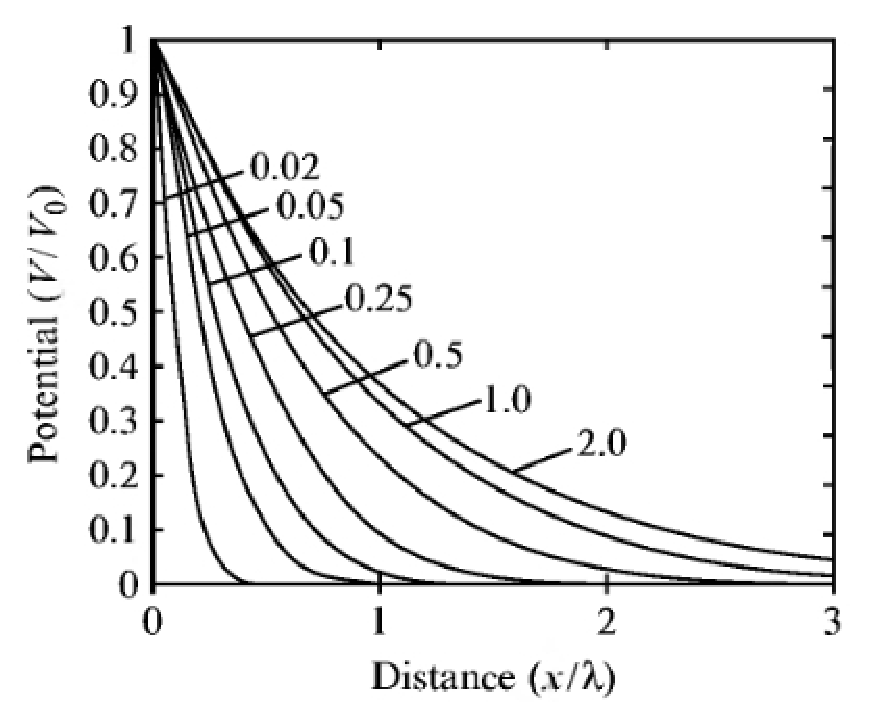
\includegraphics[height=6cm]{./images/V_standardized-x.eps}}
\caption{The numbers on the curves are the stimulus time (in units of
  membrane time-constant $\tau_m = r_m c_m$)}\label{fig:V_standardized-x}
\end{figure}

{\bf ANALYSIS 01}: \textcolor{red}{If we fixed the time which is the duration we
stimulate a signal}, the normalized solution of eq.~\eqref{eq:Vxt} is a curve
which is function of the normalized distance, as shown in
Fig. \ref{fig:V_standardized-x}. At the same stimulus time (same
curve), the potential decrease when the distance increase. The maximum
distance is reached when the potential is zero. Hence, comparing among
different curves, the longer the stimulus time, the longer the maximum
distance the signal can go. However, there is a maximum distance that
the signal can go (when $t\rightarrow \infty$).  Specifically, with
error function
\begin{equation}\begin{split}
  1 -
  \frac{2}{\pi}
  \int_0^{-\infty} e^{-y^2} dy = 2 \\
  1 -
  \frac{2}{\pi}
  \int_0^{\infty} e^{-y^2} dy = 0
\end{split}
\end{equation}
the maximum distance the signal can be transmitted is 
\begin{equation}
  V(x,t\rightarrow \infty) = V_0 e^{-\frac{x}{\lambda}}
\end{equation}

{\bf ANALYSIS 02}: \textcolor{red}{If we fixed the distance}, the normalized
solution of eq.~\eqref{eq:Vxt} is a curve which is a function of the normalized
time, as shown in Fig.\ref{fig:V_standardized-t}. At the same distance
(same curve), the longer the stimulus time, the higher the potential
when it reach that distance. The closer to the origin ($x\rightarrow
0$), the higher the potential.
\begin{figure}[htb]
\centerline{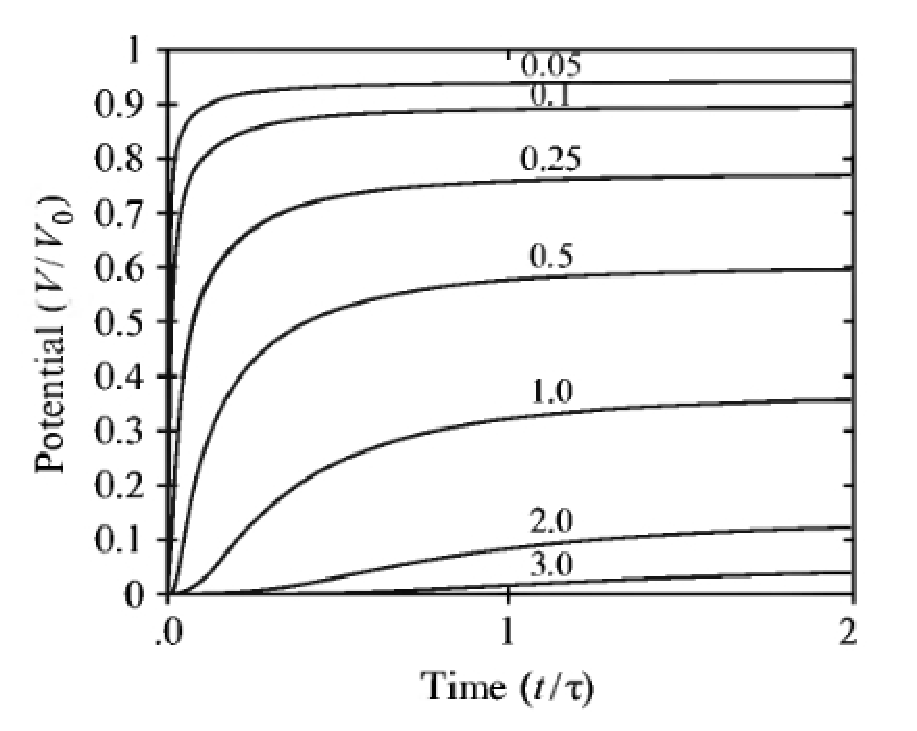
\includegraphics[height=6cm]{./images/V_standardized-t.eps}}
\caption{The numbers on the curves are the distance at which we
  measure the voltage (in units of membranes length-
  constant $\lambda = \sqrt{r_m/r_i}$)}\label{fig:V_standardized-t}
\end{figure}  



\subsection{-- the rise and fall of membrane potential}
%time constant, lengthc onstant of membrane}

\begin{mdframed}

{\bf NOTE:} Length constant ($\lambda$) is the constant used in
neurobiology. To describe the rise in potential difference across the
membrane, we use
\begin{equation}
  V = V_0 (1-e^{-x/\lambda})
\end{equation}
To describe the fall of voltage, we use
\begin{equation}
  V = V_0 . e^{-x/\lambda}
\end{equation}
Generally speaking, the length constant is the distance at which the
voltage increase 63\% (fall 37\%) of the $V_0$ during the rise (fall)
of voltage.
\end{mdframed}


{\bf NOTE:} Time constant ($\tau$) is the time it takes the system's
step response to reach approximately 63\% of its final (asymptotic)
value.

\subsection{-- Current injection}

{\bf Inject current}: Instead of having the voltage of value $V_o$ at location
$x=0$, we inject a current $I_\inj(x,t)$. Here, we uses it as a function
of space and time, to consider the general scenario that the injection can
be at any location and can change over time.

Consider the nerve cell with one axon and one dendrite at two opposite
directions. If the current of magnitude $2I_0$ (at t=0,x=0) is injected, then
the current flow in either direction should be $I_0$, parallel with the axis of
the dendrite or the axon. Then {\bf Alan Hodgkin and William Ruston} derived the
counterpart of the above equation as
\begin{equation}
  V(x,t) = \frac{\lambda R_i I_0}{2}\left( e^{-x/\lambda}
    \text{erfc}(\frac{x/\lambda}{2\sqrt{t/\tau}}-\sqrt{t/\tau}) 
    - e^{x/\lambda} \text{erfc}(\frac{x/\lambda}{2\sqrt{t/\tau}}+\sqrt{t/\tau}) 
    \right)
\end{equation}

\textcolor{red}{It's important to recognize the change of the sign on the second
term} (from + to -) inside the bracket compared with eq.~\eqref{eq:Vxt} terms.
This equation shows the {\it temporal variation of the voltage} at different
distances from the point of current injection.

{\bf NOTE:} The capacitance of the crustacean nerve membrane is about
C = $1\mu $F.cm$^{-2}$, then multiplying this by the corresponding membrane
resistance $R_m'$, we have the time constant $\tau$ about 5ms. 
\begin{equation}
  \tau = 5000 \text{ Ohm.cm}^2 \times 10^{-6} \text{F.cm}^{-2} = 5ms
\end{equation}
It means that any attempt to stimulus over a period of time shorter
than this will be thwarted by what we can loosely called
{\it system's electrical inertia}, as shown in Fig.~\ref{fig:V-tv}. In
this Figure, the membrane potential change but does not depolarized
enough to trigger an action potential.
\begin{figure}[htb]
\centerline{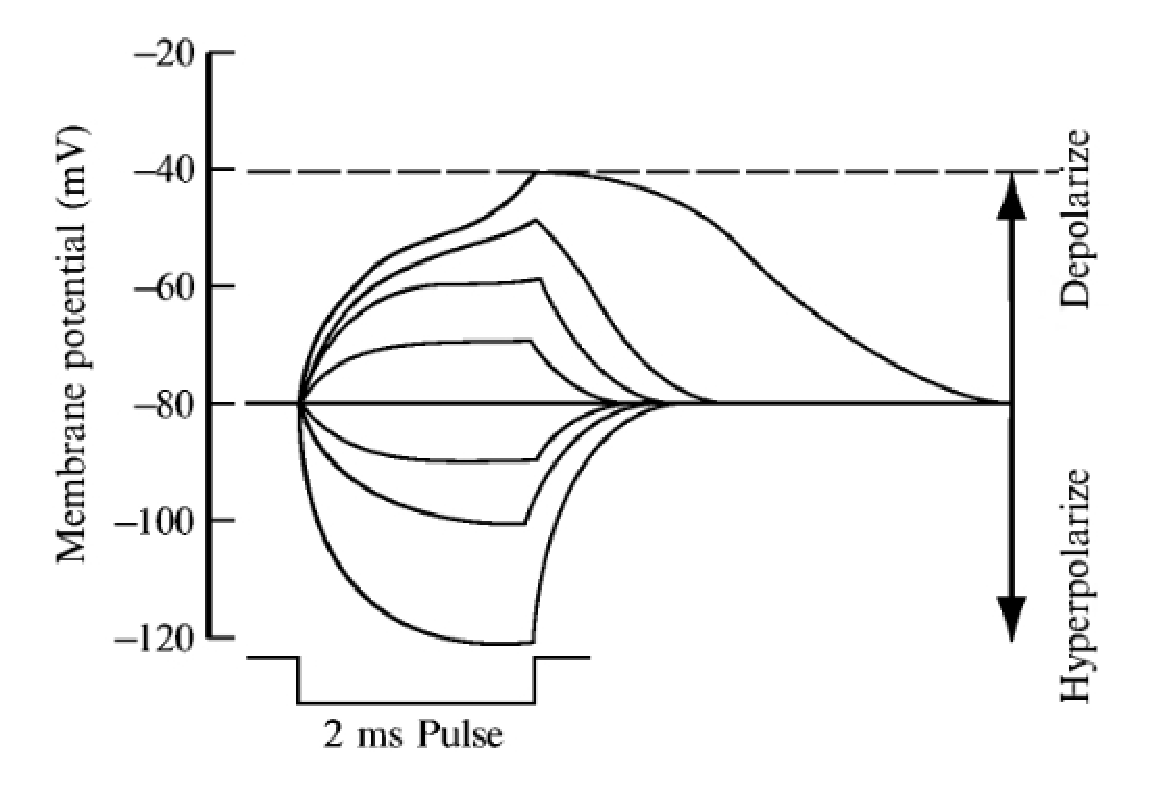
\includegraphics[height=5cm]{./images/V-temporal_variation.eps}}
\caption{Temporal variation (2ms stimulus)}\label{fig:V-tv}
\end{figure} 

\subsection{-- speed of electrical signal propagation}

The length-constant $\lambda$ and the time-constant $\tau$ determine the speed
with which an electrical signal can be {\it passively} propagated along the
nerve membrane. By passively, we mean that there is no ion channels on
the membrane or no opening of the ion channels. That speed is given by
$\lambda/\tau$ [length/time].
\begin{equation}
  \text{speed} = \lambda/\tau = \frac{4mm}{5ms} \approx 1 \qquad \text{ m/s}
\end{equation}

This is however too sluggish to response to any external signal. There should
be an error in the model. And we now know that the assumption 
$r_m =constant$ is wrong. We have to take into account the ion channels and
ion bumps which cause the variability in the resistance
(Sect.\ref{sec:complex-model-action}).

\subsection{Complex model - membrane as capacitor + ion channels}
\label{sec:complex-model-action}

By modeling the phospholipid bilayer of the membrane as a capacitor, it helps to
explain the slow decay of electrical signal as a transmembrane leak current.
However, it is still unable to explain the fast propgation of the electrical
signal.

To facilitate the fast propagation, the resistance has to be lowered.
So, the constant membrane resistance is not a correct assumption.

As a result, we have to take into account the effect of the transmembrane ion
channels and ion pumps that can significantly change the
resistance of the membrane. So, the term $\frac{V_m}{r_m}$ in eq.\ref{eq:129}
should be added the contribution from $I_\ion$ (which is not a single term but
is a combination of multiple ionic currents)

% This model was developed by Hodgkin and Huxley (1952), as shown in Fig.
% \ref{fig:Hodgkin-Huxley} (Sect.\ref{sec:Hodgkin-Huxley-1952-model}).


% The mathematical
% representation for the following assumption is called {\bf cable equation} (Sect.\ref{sec:cable_equation})


\subsection{ -- Cable equation}
\label{sec:cable_equation}

\begin{equation}
  \frac{r_m}{r_i} \frac{\partial ^2V_m}{\partial x^2} = V_m(x,t) +
  r_m c_m \frac{\partial V_m (x,t)}{\partial t} + r_m I_\inj(x,t)
\end{equation}
or
\begin{equation}
  \lambda^2 \frac{\partial ^2V_m}{\partial x^2} = V_m(x,t) +
  \tau_m \frac{\partial V_m (x,t)}{\partial t} + r_m I_\inj(x,t)
\end{equation}

NOTE:
\begin{equation}
r_i = \frac{4R_i}{\pi d^2}; \;\; r_m = \frac{R_m}{\pi d}; \;\;
c_m = \Csc \pi d
\end{equation}
then another widely used form of the cable equation is

% \begin{equation}
%   \label{eq:cable-equation}
%   \frac{R_m'}{R_i} \frac{\partial ^2V_m}{\partial x^2} = V_m + R_m'\Csc
%   \frac{\partial V_m}{\partial t} + R_m' \times I_\ion
% \end{equation}

%or if an injected current $I_\app$ is applied
\begin{equation}
  \label{eq:cable-equation}
%  \label{eq:cable-equation_full}
  \frac{d}{4R_i} \frac{\partial ^2V_m}{\partial x^2} = \frac{V_m}{R_m} + 
  \Csc \frac{\partial V_m}{\partial t} + \frac{1}{\pi d} I_\inj
\end{equation}
which is a hyperbolic PDE (Sect.\ref{sec:hyperbolic-pde}).

% \begin{itemize}
%   \item $I_m = g_\leak (V_m - E_\leak)$
%   
%   \item $I_\ion$: modeled for different types of ionic channels
%   
%   \item $I_\inj$: injected current
% \end{itemize}


\subsection{-- specific membrane capacitance $\Csc$}

Check Sect.\ref{sec:specific-membrane-capacitance}.

% \label{sec:specific-membrane-capacitance}
% 
% The specific membrane capacitance of cell membrane is approximately
% 1$\muF$/cm$^2$ and is fairly constant among different muscle cell types and
% species \citep{hille1992mb}, the membrane current density and normalized
% membrane conductance can also be represented in the form pA/pF, or mS/pF,
% respectively.
% 
% 
% % We have studied in the preceding chapter that, the ionic concentration at the
% % vicinity of the membrane are different from the bulk. As a result, each
% % leaflet of the membrane can serves as a plate of the capacitor.
% In membrane biophysics, the membrane is now considered as an electrical
% capacitor with a capacitance per unit length is $\Csc$ [Farad per unit area],
% i.e. [$\muF$/cm$^2$]. The thickness $b$ of the bilayer and the dielectric
% constant $\epsilon$ of the lipid bilayer determine the numerical value of $\Csc$. 
% (the reason for using $b$ is that it may be different from $h$ due to the
% myelin). The capacitance per surface area is
% % \begin{equation}
% % \Csc = \frac{C}{S} = \frac{k\epsilon_o}{b} = 0.01 \;\;(\text{F/m}^2)
% % \end{equation}
% 
% %The capacitance across the membrane normalized by surface takes the form4
% \begin{equation} 
% \Csc = \frac{C}{S} = \frac{\epsilon_o \kappa}{b} \;\;(\text{F/m}^2)
% \end{equation}
% with $\epsilon_o$ is the permitivity of free sapce, $\kappa$ is the
% dielectric constant of the biomembrane, and $b$ is the membrane thickness. Both
% $\kappa$ and $b$ change with membrane composition (Sect.\ref{sec:capacitance-in-neurons}).
% 
% Early estimates of $\Csc$ for biological membrane were obtained using the squid
% giant axon preparation with value $\Csc$ to be 1.0-1.3$\muF/\cm^2$. Typically,
% $\Csc=1\mu$F/cm$^2$ \citep{cole1968, weidmann1970ect}, and  has traditionally
% been viewed as a ``biological constant''. This view neglects possible
% cell-to-cell differences in the density of proteins embedded in the membrane.
% At a sufficiently high concentration, embedded proteins will increase the
% average thickness and the dielectric constant of the membrane.
% 
% $\Csc$ was treated to be 0.7-1.0 $\muF$/cm$^2$ (Koch 1999; Solsona et al. 1998). 
% \begin{enumerate}
%   \item Using artificial lipid bilayers without any transmembrane proteins, two
%   typical values of $\Csc$ are  \citep{niles1988}
% \begin{itemize}
%   \item 0.7 $\muF/\cm^2$ for membranes prepared from asolectin lipids
%   \item 0.94 $\muF/\cm^2$ for membranes prepared from egg lecithin
% \end{itemize}
% 
%   \item Using whole-cell patch clamp on mice mast cells, $\Csc$ was
% found to be 1.0 $\muF/\cm^2$ \citep{solsona1998}. 
% 
%   \item Using electro-rotation technique on spherical cultured mammalian cells
%   (suspended cells are subjected to an oscillating electric field, which causes
%   them to spin; and the rate of rotation is measured and used to estimate $\Csc$): 
%   $\Csc = 0.8 \muF/\cm^2$ \citep{sukhorukov1993}
% \end{enumerate}
% 
% In neuron, it is more difficult to measure $\Csc$ because of their
% complex morphology. 
% \begin{enumerate}
%   \item Using compartmental studies 
%   \begin{itemize}
%   \item 0.75 $\muF/\cm^2$ in hippocampal pyramidal neurons ( Major et al.,
%   1994), 
%   \item 2.4 $\muF/\cm^2$ in spinal cord ventral horn neurons ( Thurbon et al.,
%   1998) and 
%   \item 0.9 $\muF/\cm^2$ in hippocampal interneurons ( Chitwood et al., 1999)
%   \end{itemize}
% 
% These discrepancies may be due to inaccuracies in the reconstruction of
% dendritic morphology, e.g.
% confocal microscopy has shown that conventional fixation and measurement
% techniques can underestimate the surface area of the soma of adult phrenic
% motoneurons by 200\%.
% To minimize the error, \citep{gentet2008} uses nucleated patch.
%     
%   \item \citep{gentet2008} estimated the neuronal membrane to be the same 
%   $\Csc = 0.9 \muF/\cm^2$ for 3 different neuron types using nucleated patch
%   \begin{itemize}
%   \item 0.92 $\muF/\cm^2$ in nucleated patches from somatic membrane of cortical
%   pyramidal neurons (layer V), 
%   \item 0.85 $\muF/\cm^2$ in \ldots spinal cord neurons (lumbar region of spinal
%   cord), and 
%   \item 0.92 $\muF/\cm^2$ in \ldots hippocampal neurons of 7-14 day-old Wistar
%   rats, respectively.
%   \item 1.06 $\muF/\cm^2$ in cultured glial cells
%   \end{itemize}
%   Voltage-clamp protocol is used to estimate the capacitive current as a
%   single exponential time course in a nucleated patch
%   
% \end{enumerate}
% 
% \begin{mdframed}
% In myelinated axon, the myelin 
% \begin{itemize} 
%   \item  reduces the capacitance of the axon's membrane,
% from $\Csc \approx 1.0 \muF/\cm^2$. to $\Csc \approx 5.0 \times
% 10^{-3} \muF/\cm^2$.
% 
%   \item increase the resistance of unit area of membrane, from $0.2 \Omega.m^2$
%   (unmyelinated) to about $40 \Omega.m^2$ (myelinated)
% \end{itemize}
% \end{mdframed}
% 
% \citep{gentet2008} showed that increasing the protein content (i.e. about 20,000
% GlyR channels are present in the membrane of transfected HEK-293 cells with
% $\Csc = 1.11\pm 0.08$) does not change $\Csc$ (compared to untransfected HEK-293
% cells with $\Csc = 1.05\pm 0.09$), and thus suggested that, to a first
% approximation, $\Csc$ may be treated as a ``biological constant" across many
% classes of neuron.
% The estimated value of $\Csc$ was slightly larger in HEK-293 cells than in
% neurons, but this discrepancy may reflect a systematic error arising from the
% indirect estimate of HEK-293 membrane surface area.
% 
% Then, the actual value of C can be calculated by multiplying $\Csc$ with the the
% total cell membrane area. For the sake of convenience, the latter value is
% widely used $1\muF/$cm$^2$.
% 
% 
% % IMPORTANT: Specific conductance and specific capacitance are defined as ``per
% % unit area''. However, when we talk about specific resistance (or membrane
% % resistivity), we use unit ``Ohm times unit area'', e.g. Ohm.cm$^2$. Specific
% % membrane capacitance is similar in most cells and generally agreed to be
% % 0.5-1.0 $\muF$/cm$^2$  
% 
% 
% 
% \begin{figure}[htb]
% \centerline{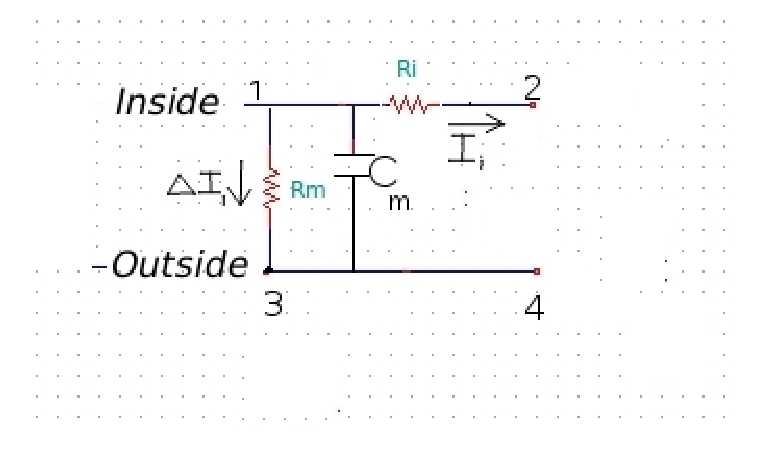
\includegraphics[height=5cm]{./images/membrane-circuit-2.eps}}
% \caption{An active nerve process $R_0 = 0$}\label{fig:circuit2}
% \end{figure}


\subsection{ -- Dimentionless the cable equation}
\label{sec:non-diment-cable}

{\bf SUMMARY}: In simple cases, we can avoid the difference in units
by non-dimensionalizing the space and time. We thus need to define new
variables $X=x/\lambda_m$ and $T=t/\tau_m$ which are both
unitless. The equation is put in the so-called
{\bf electrotonic coordinates}, i.e. we have the
{\bf unitless form of the cable equation}
\begin{eqnarray}
  \label{eq:436}
  \frac{\partial V_m}{\partial T}  =
  \frac{\partial^2V_m}{\partial X^2} + f(V_m,T)
\end{eqnarray}
with 
\begin{eqnarray}
  \label{eq:437}
  f(V_m,T) = -I_{ion}R_m
\end{eqnarray}
with $f$ is a function of both voltage and time. 



\section{A single cylinder: approximate dendrite}
\label{sec:non-isop-cell}
\label{sec:model-dendrite_cable-approximation -of-branching}
\label{sec:theor-prop}

The simple model for a single branch assumes the diameter is unchanged
along the fiber - called {\bf cable equation} (Sect.\ref{sec:cable_equation}).
At a complete dendrites, there is often branching to occur, where a single
branch is divided into two of smaller diameters. 
Due to the branching properties of the dendrite and the passive transmission of
electrical signal, the membrane potential is not considered as homogeneous along
the dendrite.

Early works of modelling nerve cells targeted to neuron with less branching,
i.e. motoneurons. One of the pioneers in this field is Wilfrid Rall
\citep{rall1962tpp, rall1969tce, rall1989ctdn, rall2006bio}.  
To deal with this, a different approach was given. This model first described
and pioneered by Rall and his colleagues. 
In this section, we will discuss the very important and beautiful
theoretical ideas of Rall.

% Steps in developing a model is that 
% \begin{itemize}
% \item test the applicability of this model to a particular case of
%   neuron by comparing with experimental data. 
% \item gain insight into the general properties of this theoretical
%   model by varying the parameters in the model to replicate pathological
%   condition of the cell
% \end{itemize}

In Rall's series of papers, he described how to map a branching dendrite into a
``mathematically equivalent'' single cylinder, and how to describe distribution
of potential in such a cylinder... using certain assumptions
\begin{itemize}
\item segments of dendrite are modeled as leaky coaxial cables
\item each parent dendrite has 2 daughter branches; the two daughter branches
have the same ``electrotonic length''. Even though this is not always true, the
empirical $\frac{3}{2}$-law is still correct.
\item $\frac{3}{2}$-law: a branching dendrite satisfy: $d^{3/2} =
  d_1^{3/2}+d_2^{3/2}$, with $d,d_1,d_2$ are the diameters of the parent and
  its two daughter branches.
\end{itemize}

\begin{framed}

The membrane space constant is defined as $\lambda = \sqrt{rR_m/2R_i}$, with $r$
is the radius of the cylinder (cm), $\Rm$ is the specific membrane resistance
(Ohm.cm$^2$), $R_i$ is the specific intracellular (axial) resistivity (Ohm.cm).
In a cable with sealed ends, the cytoplasm act as one conductor and the
extracellular space act as another one. If we assumes (not always true) that the
conductance of extracellular space may be taken as infinite, then the signal
that flows down the cable will be attenuated over the length of the axon. If $l$
is the length of the cylinder, then {\bf electrotonic length} $L$ is defined as
$L=l/\lambda$. The {\bf electrotonic distance} is different from {\bf
electrotonic length}. Electrotonic distance X is defined in the unit of
$\lambda$, i.e. if we say the electrotonic distance X of the dendrite is 1.5, it
means the length of the dendrite is $x=1.5\lambda$. Electrotonic length can
refer to any position along the cable (not just the end) to the end, but
electrotonic distance must be calculated from one end to another end.
Electrotonic length equals electrotonic distance for $x=l$. NOTE:
\textcolor{red}{the term "electrotonic distance" has no meaning when applied to
a structure of finite length, because it doesn't tell anything about how well
electrical signals spread along that structure} \citep{johnston1994fcn}.

In the case of cable equation, the voltage decay along an infinite cylindrical
cable is defined as $V(x) = V_0 \times e^{-(x/\lambda)}$. So, we can write
$X=\ln \left(V_0/V(x)\right)$. 
\end{framed}

Rall also proved that 3D distribution of potential within a dendrite can be
ignored, and it can be considered as a 1D position along the dendrite. In most
cases, extracellular potential is assumed to be fixed; including them can make
the analysis more cumbersome.  So, we can assume that a dendrite is modeled as a
one-dimensional cable, i.e. the diameter are small relative to the length. 


% \section{Theoretical proposals}

\subsection[Decay and Time-constant]{Synaptic potential decay and Soma Membrane
time constant}
\label{sec:synapt-potent-decay}

As the voltage at the soma (body) can be measured experimentally with
greater ease than those in dendrite network, and further, it is the
voltage at the soma that determine whether or not the neuron fires an
action potential, the injected current is applied directly to the soma
only.

% kha'i nie^m ban da^u ve^' action potential
In 1946, a rather simple and useful concept of ``synaptic potential''
developed by Eccles et al.~\cite{eccles1946spm}. It describes a brief
``active'' phase at the
\hyperref[chap:synapse-model-interc]{synaptic transmission}. After this
increase, the subsequent synaptic potential decay was assumed to be
passive
\footnote{ The word ''passive'' is used to imply that the membrane
  resistance, capacity, and electromotive forces all remain constant
  at their physiological resting values.}.
In other words, during the period 1946-1956, activities in the soma of
nerve cells were assumed to be subthreshold condition under the
assumption that the depolarization is uniformly distributed over the
soma membrane.
% persist of no more than 1.2ms was believed to due to a large increase
% in ionic permeability of the motoneuron membrane
% Under the assumption that the depolarization is uniformly distributed
% over the soma membrane, the soma transmembrane potential decay has the
% time constant $\tau=4$ms of the resting potential (in cat
% motoneurons).

% In motoneurons, the synaptic activation cause the dendrite to undergo
% a brief active phase of depolarization. This depolarization was
% assumed to undergo a ``passive'' decay having exponential time
% constant about $\tau = R_mC_M = 4$ ms on average (with a range from 3
% to 5ms in cat motoneurons). This active phase was believed to result
% from a large non-selective increase of the ionic permeability of the
% motoneuron membrane~\cite{rall1960mpt}.

% Now, we know that the unexpectedly low membrane time constant
% ($\tau=1.2$ms) are due to the subthreshold transient of the membrane
% potential~\cite{rall1960mpt}. 
In 1956, the rapid transient in membrane potential was first recorded
by Frank and Fuortes \cite{frank1956ssm} in cat spinal motoneurons
which was the result of a step current injected across soma membrane.
They wrongly hypothesized that the time constant of motoneurons's soma
membrane must be significant smaller (about 2.5ms) than the one
estimated based on ``synaptic
potential''\footnote{about 4ms on average and Eccles thought that it
  was due to prolonged synaptic activity}.
Thus, under the assumption that current is applied uniformly across
the soma membrane, with large enough transient in membrane potential,
the transient had been treated as simple exponential relation between
$(V/V_s)$ vs. $(t/\tau)$.
\begin{eqnarray}
  \label{eq:548}
  V =V_s (1-e^{-t/\tau})
\end{eqnarray}
In deed, as pointed out by Rall~\cite{rall1957mtc}, this is only valid
if the soma has no dendrite (known as ``soma without dendrite'') or
the current flow uniformly across the soma and dendritic membrane,
i.e. ``dendrite without soma'' (to be discussed shortly).

The fact that the soma membrane still have a high time constant,
i.e. take a long time for the current to flow across the membrane, has
been explained by Rall for the decay of the potential.  In 1960, Rall
developed a theory that ``the injected current in the soma will both
flow across the soma membrane and travel along the dendrite for
considerable distance before it flowing out across dendritic
membrane''~\cite{rall1960mpt}.

Under the subthreshold condition, we utilize the linear cable equation
for a single dendritic tree
\begin{eqnarray}
  \label{eq:452}
     \frac{\partial V}{\partial T}  =
   \frac{\partial^2V}{\partial X^2} - V
\end{eqnarray}
with $X$ is called the {\bf electrotonic distance} (electrotonic
length) along the dendritic cylinder; $X=0$ represents the
soma-dendrite junction and $V=V_m-E_r$ is the electrotonic potential
(the departure from the resting potential not exceeding the threshold
for action potential). 

Due to the assumption of soma membrane isopotential, the soma is
treated as a lumped membrane impedance at $X=0$.  Then, under the
assumption of infinite length dendritic tree, using Laplace transform,
the potential decay at the soma has the form
\begin{eqnarray}
  \label{eq:453}
  V(0,T) = \frac{V_s}{\rho-1}\left[ \rho \text{ erf
    }\sqrt{T}-1+e^{(\rho^2-1)T}\text{ erfc }(\rho \sqrt{T})\right]
\end{eqnarray}
with $\rho$ is the ratio of the combined dendritic input conductance
and the soma membrane conductance (eq.~\eqref{eq:531}), $V_s$ is the
steady state electrotonic potential (at $X=0$ during the constant
current applied) and $T=t/\tau$.

\begin{figure}[hbt]
  \centerline{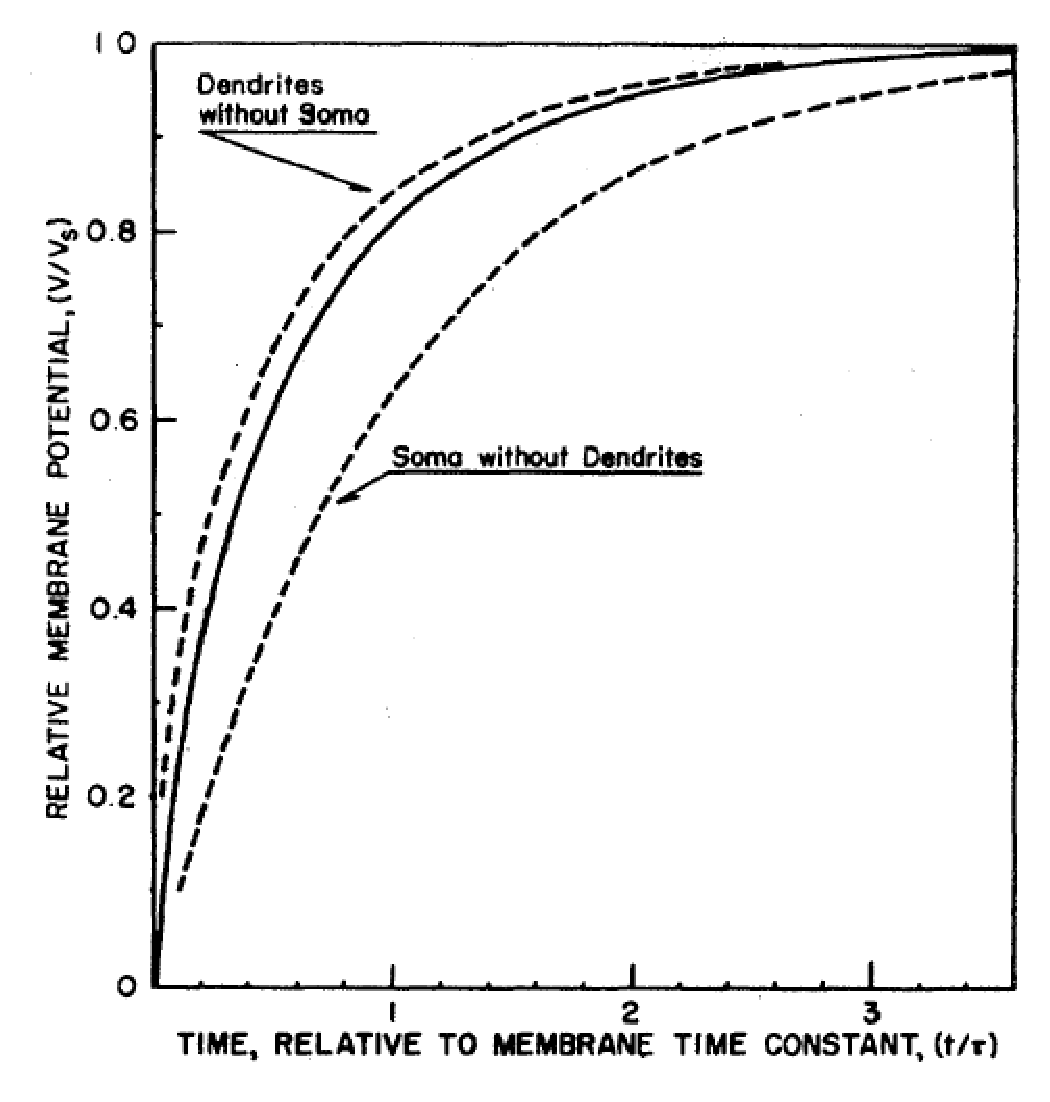
\includegraphics[height=5cm,
    angle=0]{./images/potential_soma.eps}}
  \caption{Membrane potential transient measured at soma and origins
    of dendrites (when constant current is applied uniformly across
    the soma membrane)}
\label{fig:soma_potential}
\end{figure}

There are three situations
\begin{enumerate}
\item hypothetical ``soma without dendrites'', i.e. the dendrites are
  too small, and the current flow to them are negligible 
  ($\rho \approx 0$). The curve is the lower dashed one in
  Fig.~\ref{fig:soma_potential}. Eq.~\eqref{eq:453} becomes the simple
  exponential form
  \begin{eqnarray}
    \label{eq:451}
   V(0,T) = V_S(1-e^{-t/\tau})
  \end{eqnarray}

\item hypothetical ``dendrites without soma'', i.e. dendrites dominant
  soma, and the current mainly flow to them, as shown in the upper
  dashed curve of Fig.~\ref{fig:soma_potential}. Under the theoretical
  assumptions that
\begin{enumerate}
\item All dendrites is big relative to the soma size,
\item They have same membrane time constant $\tau_m$
\item They may be represented as cylinders with infinite length. 
\end{enumerate}
This transient is well established in the theory of axonal
electrotonus and can be expressed
\begin{eqnarray*}
  V(0,T) = V_s \text{ erf } \sqrt{t/\tau}
\end{eqnarray*}
which is significantly faster than the curve in eq. \eqref{eq:451}.

\item soma with dendrites (of more practical usage). 

  Neurons do have dendrites. The ratio of the amount of current flow
  to the dendrites and those to the soma membrane depends on
  $\rho$. In motoneuron there are several large dendrites; thus a
  significant portion of the applied current must spread
  (electrotonically) along these several dendrites. As a result, it
  will change the time course of the soma membrane potential, yet
  don't know how large. % It is not simple exponential, as the time to
%   reach
% \begin{itemize}
% \item half of the steady value $V_s$ is one-third of the time
% \item 90\% of $V_s$ is three-fifths of the time
% \end{itemize}
% found in the lower dash curve.
  So, the solid middle curve represents an intermediate relation
  between the dendrite network and some, and more practical. However,
  it needs the assumption that\footnote{full discussion is given in
    the next section}
  \begin{itemize}
  \item the soma and the dendrites have the same membrane time
    constant $\tau_m$.
  \item the membrane potential at any moment is uniform over the soma
    surface, up to and including the origins of the dendrites.
  \item the dendrites can be treated as a cylinders or a structure
    which branch exponentially.
  \end{itemize}
  Nevertheless, these assumptions still underestimate the size and
  number of dendrites, thus, it is believed that the time course of
  the soma will lie between the two upper curves (for many
  motoneurons).

\end{enumerate}


% There is a difference in the time constants between that of soma
% membrane and that of synaptic potential decay.


% If the injected current is uniformly applied to the entire membrane
% surface and the hypothetical case ``soma without dendrites'', it is
% valid to assume that experimentally observed membrane transient is an
% exponential curve having this time constant $\tau$.


% \begin{eqnarray}
%   \label{eq:450}
%   V/V_s = \text{erf} \sqrt{t/\tau}
% \end{eqnarray}




\subsection{Spread of current from soma to dendritic trees}
\label{sec:spread-current-from}

Though there are several experimental results, it is not known how the
electric current spread to the dendritic trees from the soma when an
electrical current is applied inside the soma of a neuron. Some flow
across the soma membrane, some flow to the dendrite at various
distance before flowing across the dendritic membrane. A theory for
this is proposed by Rall (1959)~\cite{rall1959bdt}.

SUMMARY: The theory is general and can be applied to many types of
neurons with many types of dendritic trees (as shown in
Fig.~\ref{fig:neuron_cell}); it is also relevant to the diffusion of
material in neurons. The $3/2$ power of dendritic trunk diameter is
shown to be a fundamental index of dendritic size.
\begin{figure}[hbt]
  \centerline{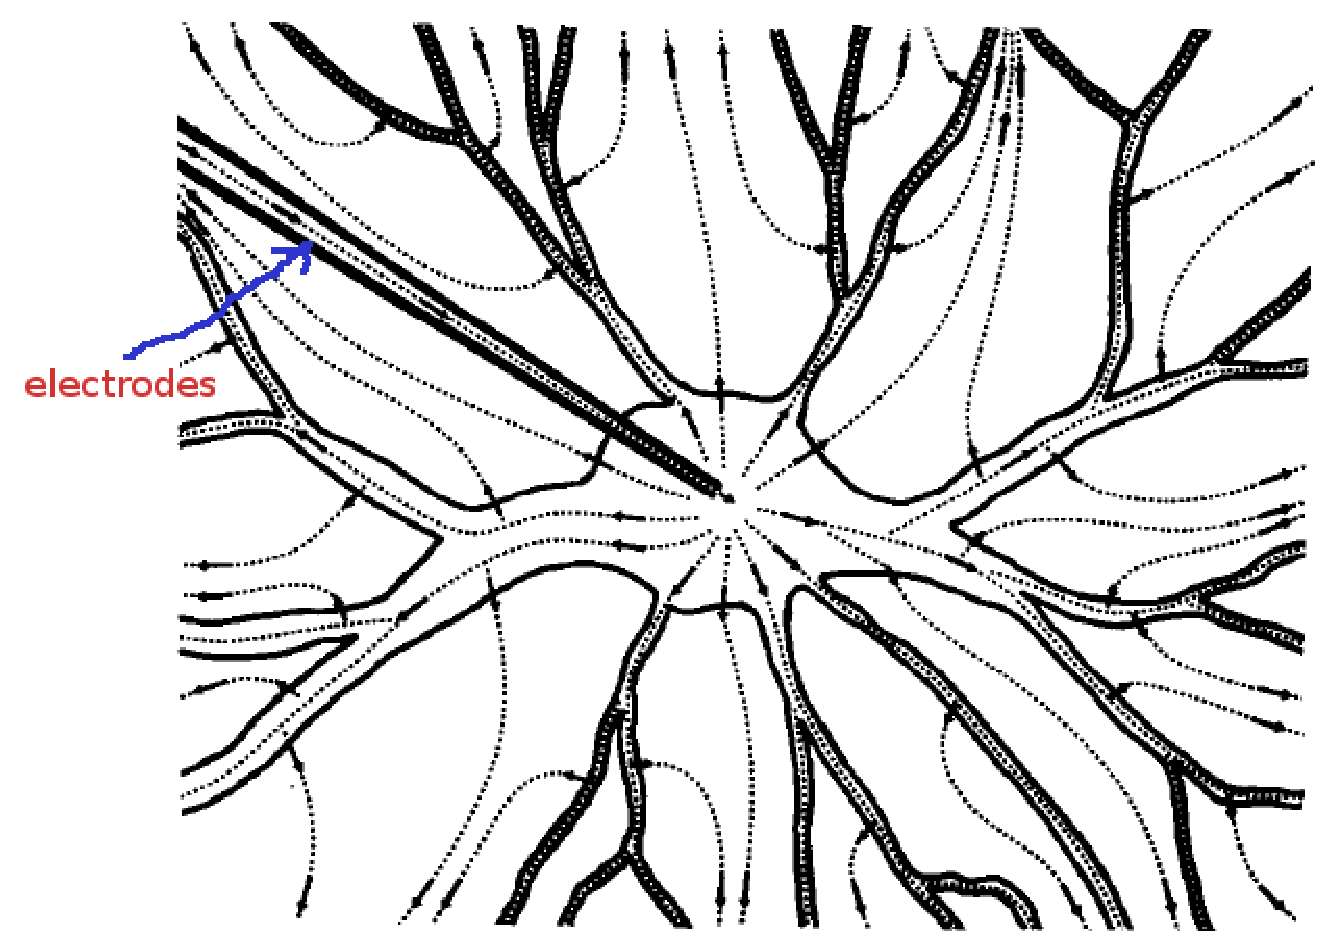
\includegraphics[height=5cm,
    angle=0]{./images/somacurrent_flow.eps}}
\caption{Diagram illustrating the flow of current from the
  microelectrode whose tips penetrate the soma of a neuron}
\label{fig:current_flow}
\end{figure}

\subsection{-- Assumptions}
\label{sec:assumptions-3}

There are different electric and geometric factors that affect the
current flows from the soma to dendritic trees.

\begin{itemize}
\item electric factors (at steady state conditions): membrane
  resistivity and specific resistivities of the intracellular and
  extracellular media, membrane capacity.

\item geometric factors: size of neuron soma, size and taper of all
  dendrite trunks, as well as amount and extent of dendrite
  branching. 
\end{itemize}

The very first models, known as ``standard motoneuron'' of Eccles
\cite{eccles1957pnc} assumed the dendrites as cylinders of infinite
length; e.g. it models a cat motoneuron with a spherical soma ($70\mu$
in diameter) with 6 dendrites of infinite length with diameter
$d=5\mu$m. A later revision added an axon ($5\mu$ diameter
cylinder)~\cite{coombs1959ecm}. However, such model and its
derivatives still underestimated the dendritic contribution by a
significant amount.

Rall proposed a theoretical model with the following 8 assumptions
(the first five is new to the model, the last three are the same as
those in the theory of axonal
electrotonus~\cite{hodgkin1946ecc})~\cite{rall1959bdt}):
\begin{enumerate}
\item the dendritic tree is assumed to consist cylindrical trunks and
  cylindrical branches, as shown in
  Fig.~\ref{fig:dendritic_tree}. It can be generalized to include
  taper.

\begin{figure}[hbt]
 \centerline{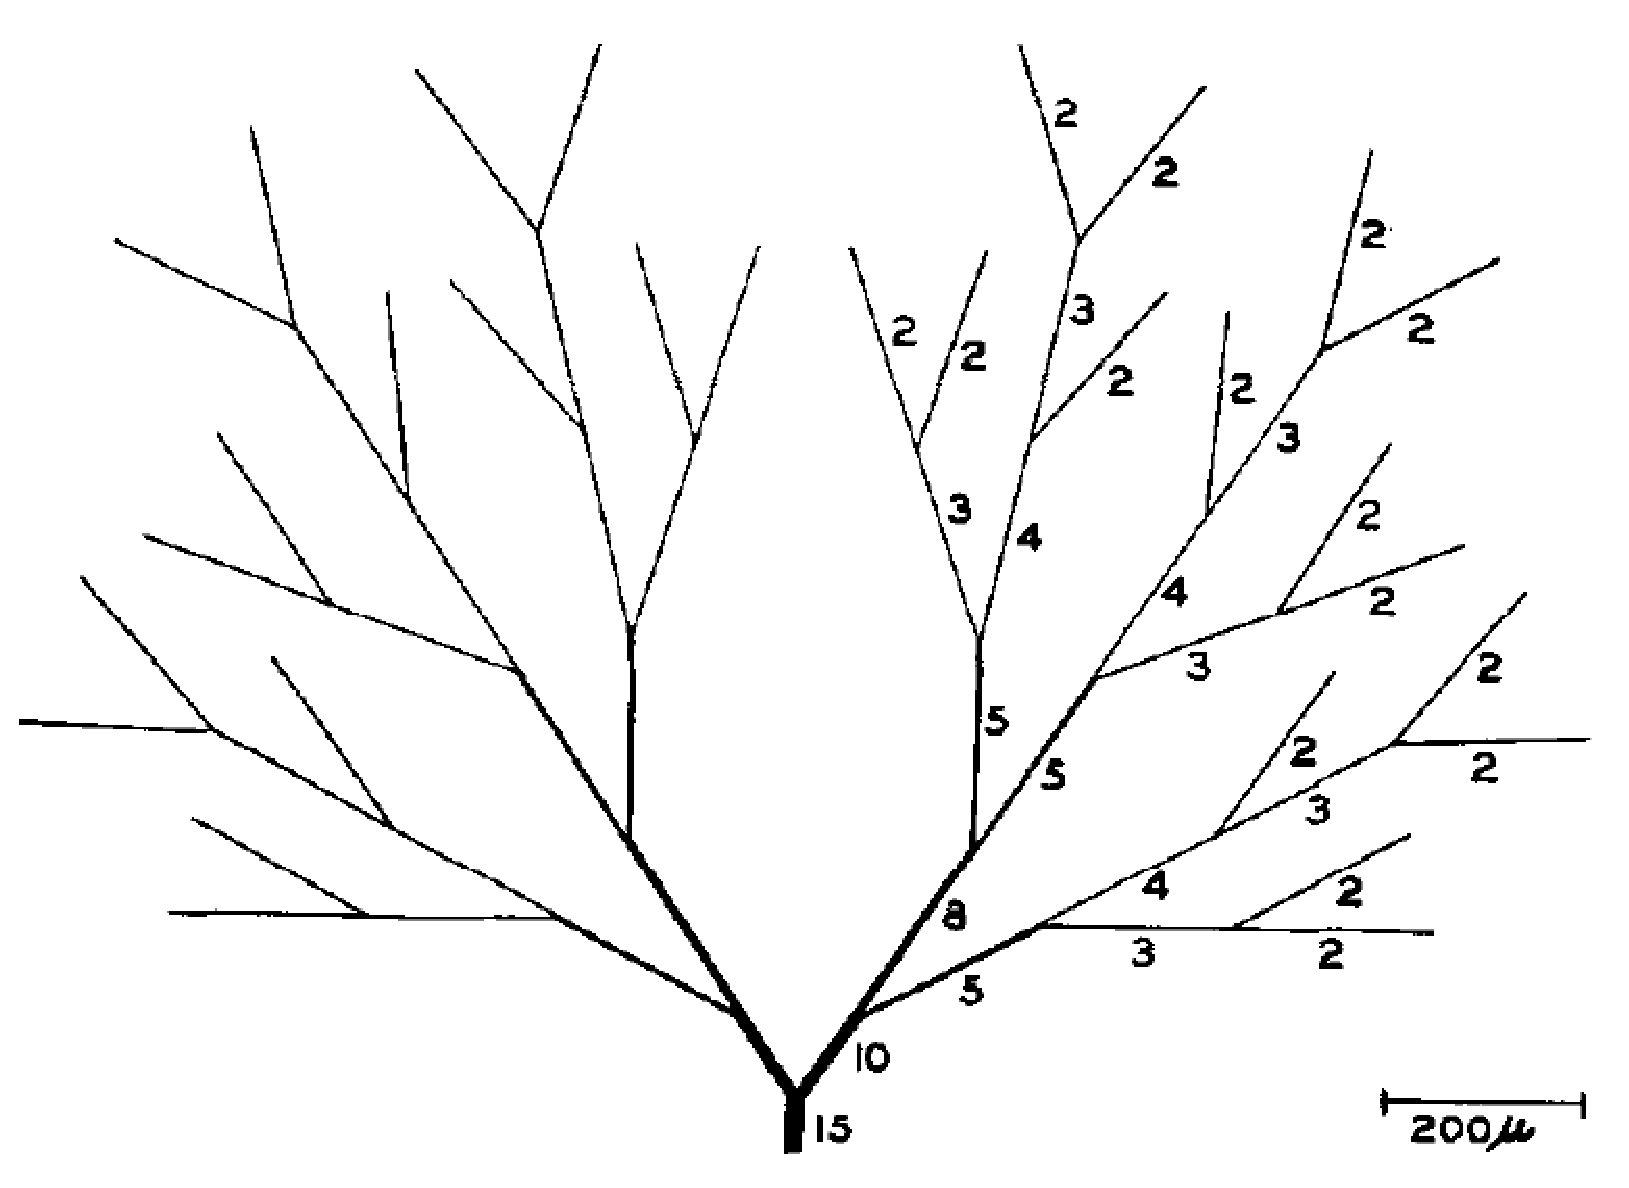
\includegraphics[height=5cm, angle=0]{./images/dendritic_tree.eps}}
 \caption{Diagram of a hypothetical dendritic tree (the two halves are
   mirror images, the numbers represent diameter in micrometers,
   trunks and all branches are assumed to be cylinders). Main trunk is
   50$\mu$m in length, bifurcates into 2 branches, each with
   $100\mu$m in length; all next branches, for simplicity, are assumed
   to be $200\mu$m in length. This 2D tree is meant to represent a more
   compact 3D tree}
\label{fig:dendritic_tree}
\end{figure}

\item electric properties are assumed to be uniformed over the entire
  {\it soma-dendritic surface}.

\item isopotential of external
  medium\footnote{the gradient of external potential is supposed to be
    very small compared to the axial internal gradient of potential}
  ($V_e=\text{const}$, or $r_e=0$). See
  \hyperref[sec:disc-homog-vs]{discussion}.
% (electric potential is assumed
%   to be constant and uniformly distributed over the entire external
%   surface of the neuron)

\item isopotential of internal medium ($V_i=\text{const}$). Based on
  this and the 3rd assumption, the membrane voltage is a constant and
  thus is independent from the soma surface. Thus, the entire soma
  membrane can be lumped into a membrane impedance that represents the
  common origins for all dendrite trunks belonging to this neuron.

\item internal potential and currents are assumed to be continuous at
  all dendritic branching points and all soma-dendritic
  junctions\footnote{importance for mathematical treatment}.

\item electric current inside any cylindrical component is assumed to
  flow axially through an ohmic resistance $r_i$ which is inversely
  proportional to the cross section area $A_i$ ($r_i=\frac{R_c}{A_i}$
  with $R_c=R_i$ as cytoplasmic resistivity)

\item the electric current across the membrane is assumed to be normal
  to the membrane surface, i.e. an ohmic resistance in parallel with a
  perfect capacity.

\item membrane electromotive force $E_r$ is assumed to be in series
  with membrane resistance, and is assumed to be constant for all of
  the membrane. Under the steady state condition and no current flow,
  the resting potential of the membrane is $V_{rest} = E_r$.
\end{enumerate}

Based on these 8 assumptions, we can derive the linear cable equation
\begin{eqnarray}
  \label{eq:454}
  \frac{\partial V}{\partial T}  = \frac{\partial^2V}{\partial X^2} - V
\end{eqnarray}
with $V=V_m-E_r$ is the electrotonic potential, $X=x/\lambda$ is the
electrotonic distance along the cylinder, and $T=t/\tau$. The
procedure has been described in Sec.~\ref{sec:non-isop-cell}. To solve
this problem, we need the initial and boundary conditions, which can
be referenced in Sec.~\ref{sec:boundary-condition}.

\subsection{-- Solution under steady state condition}
\label{sec:solut-under-steady}

Now, we examine eq.~\eqref{eq:454} under steady state condition,
$\frac{\partial V}{\partial T} = 0$, using Fig.~\ref{fig:lumped_soma}.

\begin{enumerate}
\item For the dendritic trunk ($x<x1$), the general solution can be
  expressed in terms of the exponential or hyperbolic function
\begin{eqnarray}
  \label{eq:457}
  V/V_1 = \cosh\left[ (x_1-x)/\lambda_0 \right] + 
  B_1 \sinh \left[ (x_1-x)/\lambda_0\right]
\end{eqnarray}
with $\lambda=\lambda_0$ is the characteristic length specifically to
the dendritic trunk; $V_1$ is the value of $V$ at $x=x_1$; and the
constant $B_1$ is the amount of axial current flowing at
$x=x_1$. Thus,
\textcolor{red}{$B_1$ depends upon branching} (to be discussed
  shortly).

\item For the soma ($x=0$), a reduced form of eq.~\eqref{eq:457} is
  \begin{eqnarray}
    \label{eq:458}
    V_0/V_1 = \cosh (x_1/\lambda_0) + B_1 \sinh (x_1/\lambda_0)
  \end{eqnarray}
  with $V_0$ is the soma electrotonic (subthreshold) potential.
\end{enumerate}
\begin{figure}[hbt]
  \centerline{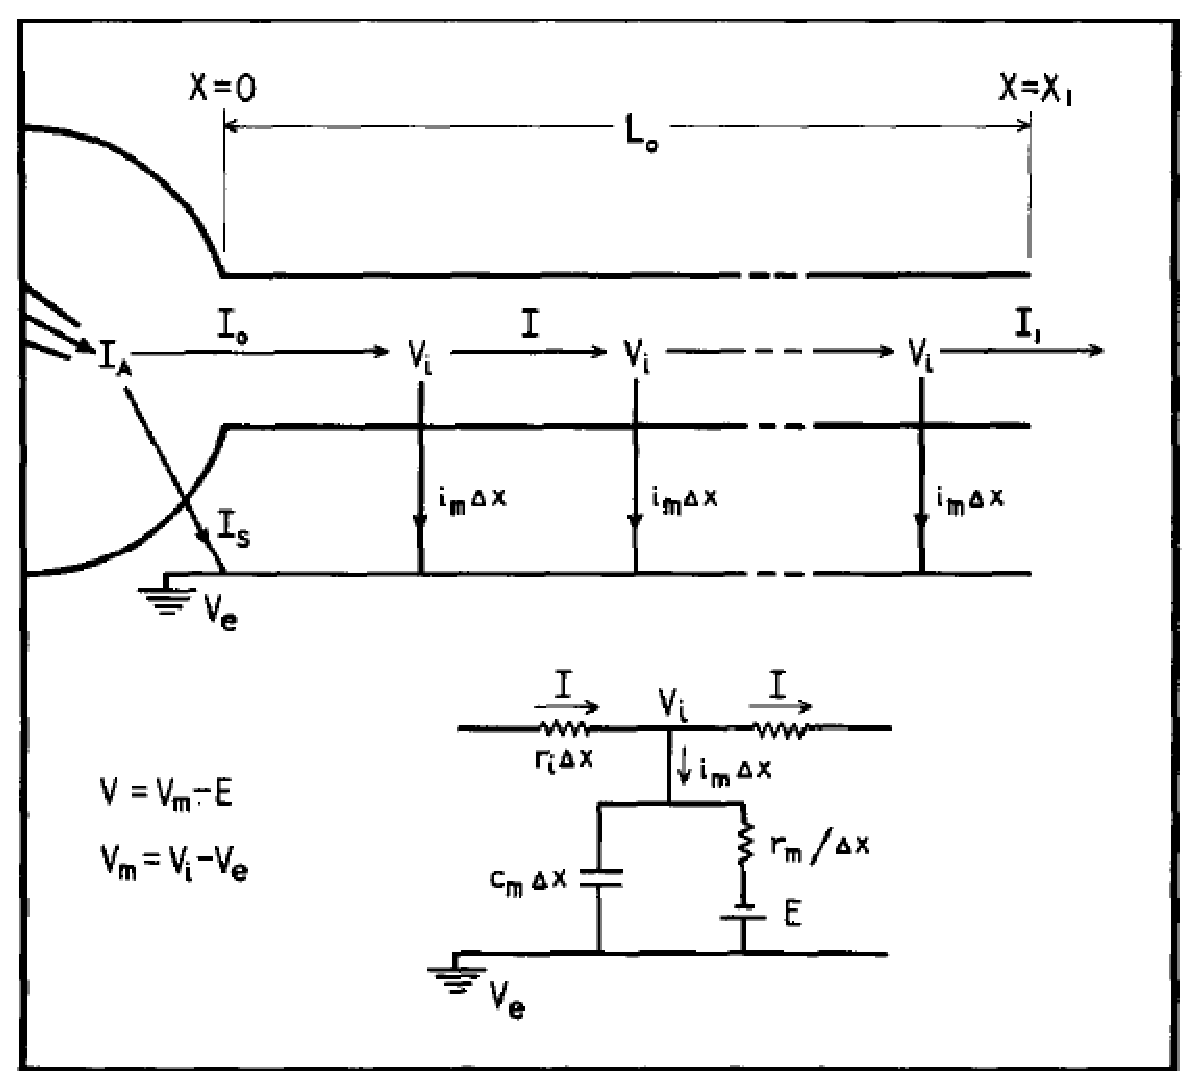
\includegraphics[height=5cm,
    angle=0]{./images/lumped_soma.eps}}
\caption{Electric potential and current flow for a cylindrical trunk
  arising from the soma.}
\label{fig:lumped_soma}
\end{figure}

If there is no branching ($B_1=1$), eq.~\eqref{eq:458} becomes the
function of potential decay in axonal cylinders (of infinite length)
\begin{eqnarray}
  \label{eq:459}
  V/V_0 = e^{-x/\lambda_0}
\end{eqnarray}
For a dendritic trunk, even though it has infinite length, it can
branch. Thus, the eq.~\eqref{eq:459} apply only for the range 
$0\le x\le x_1$, i.e. the branches arising at $x=x_1$. 
The value $B_1>1$
implies that the dendritic tree is branched more extensively than
this, and $B_1<1$ means a less branching, e.g. termination. Let's
examine the situation of termination of cylinder: (1) $B_1=0$
(``sealed end''), (2) $B_1=\infty$ (``killed end'').

\begin{enumerate}
\item $B_1=0$
  \begin{eqnarray}
    \label{eq:460}
    V/V_0 = \frac{\cosh[(x_1-x)/\lambda_0]}{\cosh(x_1/\lambda_0)}
  \end{eqnarray}

When the membrane cylinder is sealed with a disc composed of the same
membrane, the exact solution for $B_1$ is
\begin{eqnarray*}
  B_1=\lambda_0\frac{R_i}{R_m}
\end{eqnarray*}
Given $R_1=50\Omega$.cm, $R_m=1250\Omega$cm$^2$, $d_0=4\mu$m, then
$B_1=2\times 10^{-3}$ which is almost zero. Thus, $B_1=0$ is a good
approximation for the boundary condition ``sealed end'', i.e. very
high resistance between the internal and external media at $x=x_1$ or
equivalently no membrane current at that point.

\item $B_1=\infty$
  \begin{eqnarray}
    \label{eq:461}
    V/V_0 = \frac{\sinh[(x_1-x)/\lambda_0]}{\sinh(x_1/\lambda_0)}
  \end{eqnarray}
  which corresponds to the voltage-clamped boundary condition
  $V_1=-E_r$. The exact value for $B_1$ is
  \begin{eqnarray*}
    B_1 = \lambda_0R_i/R_m =\left[ (R_i/R_m)(d_0/4)\right]^{1/2}
  \end{eqnarray*}
  with $\lambda_0=\sqrt{(R_md_0)/(4R_i)}$, and $d_0$ is the diameter
  of the dendrite trunk.

\item Given two boundary conditions $V=V_0$ ($x=0$), and $V=-E_r$
  ($x=x_1$)
  \begin{eqnarray}
    \label{eq:462}
    V = \frac{V_0\sinh \left[ (x_1-x)/\lambda_0\right] - E_r\sinh (x/\lambda_0)}{\sinh (x_1/\lambda_0)}
  \end{eqnarray}
\end{enumerate}

\subsection{-- Axial currents}
\label{sec:axial-current}


\begin{mdframed}

IN GENERAL CASE: Remember that there are conducting pores across the membrane,
i.e. receptor or ion channels. For the purposes of the analysis we shall carry
out, it suffices to consider the lumped resistance of the cell without regard to
the various reversal potentials $E_i$ with i = Na, Cl, K.

Current flow in a resistor is of course governed by Ohm's law: $I=V/R=g.V$.
NOTE: Resistors in series sum, while resistors in parallel combine
`reciprocally' $R_\text{tot}=\frac{1}{1/R_1 + 1/R_2}$, the combination of all
the conducting system can be represented as a membrane resistance $R_m =
\frac{R_M}{A}$ with $R_M$ is specific membrane resistance (Ohms.m$^2$ -
Sect.\ref{sec:specific-membrane-resistance}), and $A$ is membrane surface area,
Fig.\ref{fig:membrane_RC}.
\end{mdframed}

Under the assumption of core conductor (Sect.\ref{sec:core-conductor-model}),
there are only two types of currents: one transmembrane current ($I_m$) and two
axial currents ($I_i$ and $I_e$).


{\bf CONSIDER AXIAL CURRENTS} (x-axis): There are two axial currents:
intracellular $I_i$ and extracellular $I_e$ components, which are assumed to be
linear functions of the voltage.

Assuming the segment of length $\Delta x$
\begin{equation}
  \label{eq:421}
  \begin{split}
    V_i(x+\Delta x)-V_i(x) &= -R_i \times I_i(x)\\
    V_e(x+\Delta x)-V_e(x) &= -R_e \times I_e(x)\\
  \end{split}
\end{equation}
with $R_i=R$ (Ohm), $R_e$ (Ohm), $I_i(x)$ (A), and $I_e(x)$ (A).
The minus sign appears on the right-hand size because of the convention that
positive current is the flow of positive charges from the left to the right
(i.e. in the direction of increasing $x$).

The equivalent form, 
\begin{equation}
  \label{eq:421_b}
  \begin{split}
    \frac{V_i(x+\Delta x)-V_i(x)}{\Delta x} &= -\frac{R_i}{\Delta x} \times I_i(x)\\
    \frac{V_e(x+\Delta x)-V_e(x)}{\Delta x} &= -\frac{R_e}{\Delta x} \times I_e(x)\\
  \end{split}
\end{equation}

In the limit of a segment of an infinitestimal small length $\Delta x$
$\rightarrow 0$,
\begin{equation}
  \label{eq:422}
  \begin{split}
    I_i &= -\frac{1}{r_i}\frac{d V_i}{d x} \\
    I_e &= -\frac{1}{r_e}\frac{d V_e}{d x} \\
  \end{split}
\end{equation}
with 
\begin{itemize}
  \item $r_i = R/\Delta x$ is intracellular resistance per unit length of cable
[Ohm/cm]

  \item $r_e = R_e/\Delta x$ is extracellular resistance per unit length of
  cable [Ohm/cm]
\end{itemize}

NOTE: \textcolor{red}{Here, the voltage is only the function of distance}
$V_i(x)$, 
% By using the Ohm law for the axial current:
% $  I_i(x) = \frac{V_i(x) - V_i(x+\Delta x,t)}{R_i^0} $, then
% \begin{equation}
%   \label{eq:Ohm-law}
%  -I_i(x) = \frac{d  V_i(x)}{R_i^0} =  \frac{d  V_i}{R_i\times
%  d x}
% \end{equation} 
with $d  V_i = V_{i,1}-V_{i,2}$ is 
the difference potential between two
ends of the small segment of the cylinder at a distance $\Delta x$ 
(NOTE: $V_1$ is near the starting end). 

At any node (point) between two adjament segments, the currents must balanced,
using Kirchoff law which states that the sum of all currents flowing into and
out of any node must equal zero.
\begin{equation}
i_m(x,t) + I_i(x,t) - I (x-\Delta x, t) = 0
\end{equation}
and in differential form ($\Delta x \rightarrow 0$)
\begin{equation}
  \label{eq:43}
  i_m(x,t) = I_m =   -\frac{dI_i}{dx} 
\end{equation}

We take a derivative of eq. \ref{eq:422} to get the right-hand side of
eq.\ref{eq:43}.

% We can write eq.~\eqref{eq:Ohm-law} in
% the form of derivative
% \begin{equation}
%   -I_i = \frac{1}{R_i} \times \frac{d V}{d x}
% \end{equation} 
% or 
\begin{equation}
  \label{eq:dIidx}
  -\frac{dI_i}{dx} =  \frac{1}{r_i}\frac{d ^2V_i(x)}{d x^2}
\end{equation} 

% As we assume there are only two types of currents, intracellular
% current and transmembrane current, using Kirchoff law, the loss in the axial
% current should be the transmembrane current $I_m$.
% In other words, we have
% \begin{equation}
%   \label{eq:43}
%   -\frac{dI_i}{dx} = I_m
% \end{equation}

\begin{mdframed}

In this case: in addition to the resistance of the membrane $R_m$, we also have
the resistance of the cytoplasm $R_i$ and the extracellular space $R_o$. For the
sake of simplicity, the extracellular is assumed to be isopotential, i.e. no
resistance $R_e=R_o=0$ in most of the cases. This is based on the assumption
that the extracellular space is either a perfect conductor or of infinite
extent.
However, in some special problems, e.g. the tightly packed axons in a nerve
trunk or for neurons in a CNS where the current flow in the extracellular may be
significant, $R_o$ may be non-zero.
\end{mdframed}

Consider $V_m = V_i - V_o$ is the transmembrane potential, so,
\begin{equation}
  \label{eq:126}
%  I_m =  \frac{V_m}{R_m^'} = \frac{V_m}{R_m .h}
  i_m =  \frac{V_m}{r_m}
\end{equation}
% with $R_m'=R_m^0\times h$ [Ohm.m].
% with [$I_m$] = [A/m], [$R^0_m$]=[Ohm].


NOTE: As $V_e(x)= const$, 
$\Delta V = V_1-V_2 = (V_1 - V_{out}) - (V_2 -V_{out}) = V_{m,1} = V_{m,2} =$
$\Delta Vm$, or $d V = d V_m$.
Combine this with eq.\ref{eq:126} and eq.\ref{eq:43} and eq.\ref{eq:dIidx}:
\begin{equation}
  \label{eq:127}
  V_m = \frac{r_m}{r_i} \frac{d ^2V_m}{d x^2}
\end{equation}

\begin{mdframed}[linecolor=red!60!black,  linewidth=2pt]

To make it simple, we assume the outside medium has $R_{0} =
0$, so $V_{out}= 0$ or $V_m = V_x$. 
The general solution of ~\eqref{eq:127} is
\begin{equation}
  V_x = A.\exp \left( \frac{-x}{\sqrt{r_m/r_i}} \right) +  B.\exp
  \left( \frac{x}{\sqrt{r_m/r_i}} \right)
\end{equation}

% TODO: find the meaning of B in second term ?

{\bf What are the values of A, B?}: In a passive cable (i.e. membrane
conductance is not a function of $\Vm$), $V_x$ tends to zero when
$x\rightarrow \infty$. So we can eliminate the second term, i.e. $B=0$.
\begin{equation}
   V_x = A.\exp \left( \frac{-x}{\sqrt{r_m/r_i}} \right) 
\end{equation}

\end{mdframed}

Assuming that at one end of the axonal process, the initial potential
is $V_x = V_0$, at $x=0$. Then, $A = V_0$ or
\begin{equation}
  \label{eq:128}   
 V_x = V_0.\exp \left( \frac{-x}{\sqrt{r_m/r_i}} \right) 
\end{equation}
The term in the exponent should be unitless. This is true since
[$r_m$]=[Ohm.cm] while [$r_i$]=[Ohm/cm], using \eqref{eq:resistance},
we have
\begin{equation}
  \sqrt{r_m/r_i} = \sqrt{\frac{\rho_m\Delta
      x h}{2\pi.r.h}/\frac{\rho_i}{\pi.r^2}} = \sqrt{r\rho_m\Delta x/2\rho_i}
\end{equation}
So, the thickness of the membrane is canceled out, and is thus not play a role
to the decay of the voltage. Next, we define:
\begin{equation}\label{eq:rhom}
  \rho_m' = \rho_m. \Delta x
\end{equation}
with $\rho_m$ is the resistivity of the membrane so that we can use it
to compute $r_m$.


Based on assumption 6, the axial current follow the ohmic resistance
\begin{eqnarray*}
  I = -\frac{\partial V}{\partial x}(1/r_i)
\end{eqnarray*}
with $0\le x\le x_1$. Taking the first-order derivative of
eq.~\eqref{eq:457}, the axial current $I$ is given in
\begin{eqnarray}
  \label{eq:463}
  I/V_1 = G_\infty \left\{ \sinh [(x_1-x)/\lambda_0] + B_1 \cosh [(x_1-x)/\lambda_0]\right\}
\end{eqnarray}
with

\begin{eqnarray*}
  G_\infty &=& (\lambda_0r_i)^{-1} \\
  &=& (\pi/2)\frac{1}{(R_mR_i)^{1/2}} (d_0)^{3/2}
\end{eqnarray*}
corresponds to the infinite extension of the cylindrical trunk.  Then,
the input current from the soma to the dendritic $I_\inj(x,t) $ can be obtained
from eq.~\eqref{eq:463} by setting $x=0$. 

The dendritic input conductance for a single dendritic tree
\begin{eqnarray}
  \label{eq:464}
  G_D = I_\app /V_0=B_0G_\infty
\end{eqnarray}
where 
\begin{eqnarray*}
  B_0 = \frac{B_1+\tanh(L_0/\lambda_0)}{1+B_1\tanh(L_0/\lambda_0)}
\end{eqnarray*}
with $L_0=x_1$. 

{\bf NOTE}: We use $L_0$ so that it can be adapt to any branch of
length $L_i$.
\begin{enumerate}
\item If $B_1=1$, then $B_0=1$ (unity).
\item If $B_1=0$ (``sealed end''), then $B_0=\tanh(L_0\lambda_0)$
  (smallest possible value of $B_0$) or $G_D\le G_\infty$.
\item If $B_1=\infty$ (``killed end''), then
  $B_0=\coth(L_0/\lambda_0)$ (largest possible value of $B_0$) or
  $G_D\ge G_\infty$.
\end{enumerate}

\subsection{-- Branching dendritic tree}
\label{sec:branch-dendr-tree}



\begin{figure}[hbt]
  \centerline{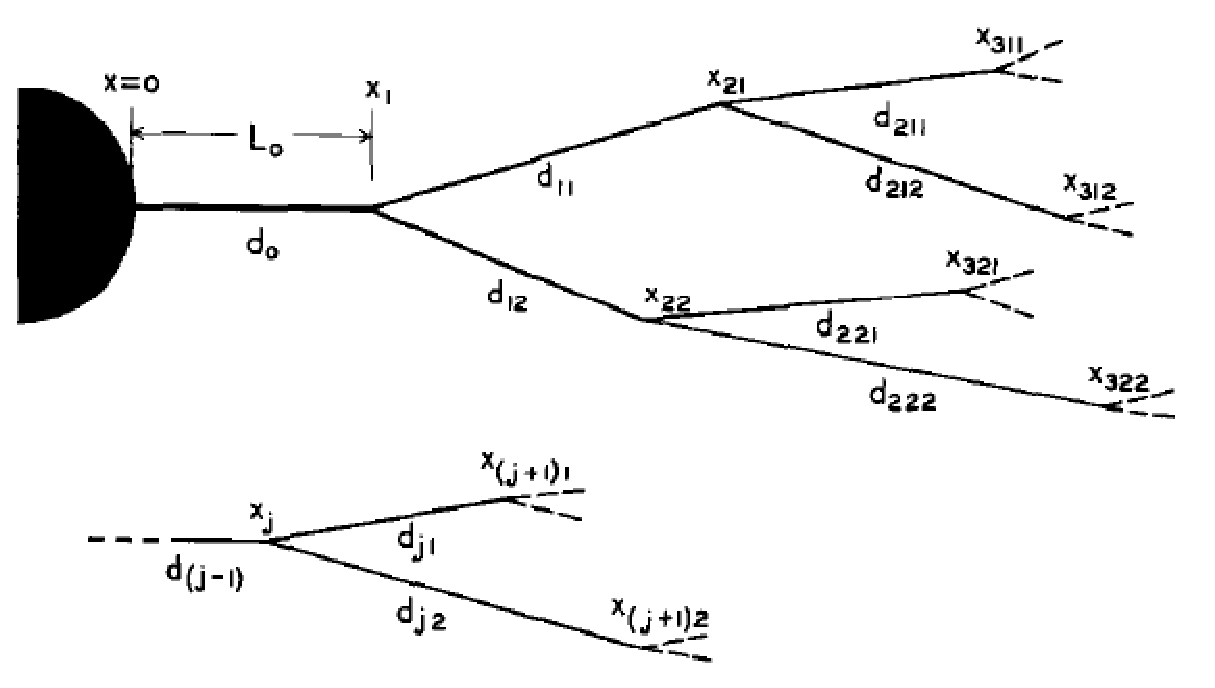
\includegraphics[height=5cm,
    angle=0]{./images/dendritic_branching.eps}}
\caption{Dendritic branching}
\label{fig:dendritic_branching}
\end{figure}

Now, we examine branching, as shown in
Fig.~\ref{fig:dendritic_branching}.  The input current to the next
branching is the current at $x=x_1$ which is simply a reduced form of
eq.~\eqref{eq:463}
\begin{eqnarray}
  \label{eq:467}
  I_1/V_1 = B_1 G_\infty
\end{eqnarray}
For each branching at $x=x_1$, say the $k$-th branch, i.e. extending
from $x=x_1$ to $x=x_{2k}$, having
\begin{enumerate}
\item diameter $d_{1k}$
\item length $L_{1k}$
\item characteristic length $\lambda_{1k}$
\end{enumerate}
Then
\begin{eqnarray}
  \label{eq:465}
  I_{1k}/V_1 = B_{1k} G_\infty (d_{1k}/d_0)^{3/2}
\end{eqnarray}
and
\begin{eqnarray}
  \label{eq:466}
  B_{1k}  = \frac{B_{2k}+\tanh(L_{1k}/\lambda_{1k})}{1+B_{2k}\tanh(L_{1k}/\lambda_{1k})}
\end{eqnarray}
Based upon the assumption (5), the sum of all branching current must
be equal to the one at the parent dendritic branch, thus
\begin{eqnarray*}
  I_1 &=& \sum_k I_k   
\end{eqnarray*}
Combine this with eq.~\eqref{eq:467} and eq.~\eqref{eq:465}, we have
\begin{eqnarray}
  \label{eq:469}
  B_1 &=& \sum_k B_{1k} (d_{1k}/d_0)^{3/2}
\end{eqnarray}

We then can generalize to any branch point, starting at $x=x_j$, and
ending at $x=x_{j+1}$
\begin{eqnarray}
  \label{eq:468}
  B_j = \sum_k B_{jk} \left[d_{jk}/d_{(j-1)}\right]^{3/2}
\end{eqnarray}
where 
\begin{eqnarray*}
  B_{jk} = \frac{B_{(j+1)k} + \tanh(L_{jk}/\lambda_{jk})}{1+B_{(j+1)k}\tanh(L_{jk}/\lambda_{(jk})}
\end{eqnarray*}
with the subscript $jk$ represents the $k$-th branch arising at
$x=x_j$; and
\begin{eqnarray}
  \label{eq:470}
  \lambda_{jk} = \left[ (d_{jk}/4)(R_m/R_i)\right]^{1/2}
\end{eqnarray}

{\bf IMPORTANT NOTE}: Any $B_{jk}$ value different from unity always
lie between $B_{(j+1)k}$ and unity. Once a value close to unity is
reached, further steps cannot carry the value away from unity by any
significant amount.


\subsection{-- Whole neuron conductance}
\label{sec:whole-neur-cond}

\begin{eqnarray}
  \label{eq:471}
  G_N = I_A/V_0 = 1/R_N
\end{eqnarray}
with $I_A$ is the applied current flowing from an electrode within the
neuron soma to an extracellular electrode, $V_0$ is the steady state
electrotonic potential at $x=0$ under the constant $I_A$.

Again, using assumption (5), we have
\begin{eqnarray}
  \label{eq:472}
  I_A = \sum_k I_{k} + I_m
\end{eqnarray}
with $I_k$ the current at dendrite tree $k$-th, and $I_m$ the current
across the soma membrane

Based on the assumption (2-4), the conductance is uniformly
distributed across the membrane surface
\begin{eqnarray}
  \label{eq:473}
  G_S = S/R_m
\end{eqnarray}
with $S$ the soma surface area.  The total dendritic conductance
(using eq.~\eqref{eq:464})
\begin{eqnarray}
  \label{eq:474}
  \sum_j G_{D,j} = CD^{3/2}(R_m)^{-1/2}
\end{eqnarray}
where
\begin{eqnarray}
  \label{eq:475}
  C &=& (\pi/2) R_i^{-1/2} \\
  D^{3/2} &=& \sum_j B_{0,j}(d_{0j})^{3/2}
\end{eqnarray}
with all dendritic tree have the same $R_i$.

{\bf REMARKS}: Eq.~\eqref{eq:475} shows that the combined effect of
several dendritic trees is proportional, not to a simple sum or
average of the trunk diameters $d_{0j}$, but to a sum composed of the
3/2 power of each trunk diameter appropriately weight with the
weighting factor $B_{0j}$. However, as $B_{0j}$ depends upon
$R_m/R_j$, to have a purely geometric characteristic of the dendritic
trees, it's useful to use~\cite{rall1959bdt}
\begin{eqnarray}
  \label{eq:480}
  \sum_j d_{0j}^{3/2}
\end{eqnarray}
\textcolor{red}{This had revealed the important role of the 3/2 power
  of the diameter of each branch cylinder}.

Finally, the whole neuron conductance is given
\begin{eqnarray}
  \label{eq:476}
  G_N = CD^{3/2}(R_m)^{-1/2} + S/R_m
\end{eqnarray}
with the assumption that both soma and dendrite membrane have the same
$R_m$. 

As $R_N$ can be measured experimentally, the estimating for $R_m$ can
be derived from eq.~\eqref{eq:476}
\begin{eqnarray}
  \label{eq:477}
  R_m = (1+\epsilon) C^2 D^3 R_N^2
\end{eqnarray}
with 
\begin{eqnarray}
  \label{eq:478}
  1+\epsilon = \frac{1}{4}\left[ 1 + \sqrt{1+\frac{4S}{C^2D^3R_N}} \right]^2
\end{eqnarray}

\subsection{-- Accumulated dendritic conductance to soma conductance
  ratio}
\label{sec:dendr-soma-cond}

The ratio $\rho$ as mentioned in the previous sections is
\begin{eqnarray}
  \label{eq:531}
  \rho = \frac{\sum_j G_{D,j}}{G_S}
\end{eqnarray}

Finally, the {\bf dendritic to soma conductance ratio}
(eq.~\eqref{eq:473} and eq.~\eqref{eq:474})
\begin{eqnarray}
  \label{eq:479}
  \rho = C\left[D^{3/2}S \right]\sqrt{R_m}
\end{eqnarray}
This ratio depends upon both geometric and electric quantities. Given
that $D^{3/2} = \sum d_{0j}^{3/2}$, a purely geometric parameter, the
quantity $D^{3/2}/S$ is also considered as purely geometric.

When $R_m$ is assumed, we can find $\rho$ via
\begin{eqnarray}
  \label{eq:481}
  R_N = \frac{R_m}{(\rho+1)S}
\end{eqnarray}
Though further anatomical tests need to be performed to judge the
accuracy of the formula, the idea is very elegant.

% Based on those 8 assumptions, we have
% \begin{eqnarray}
%   \label{eq:456}
%   \lambda = \sqrt{r_m/r_i}\\
%   r_m = \frac{R_m}{\pi d}\\
%   r_i = \frac{4R_i}{\pi d^2}
% \end{eqnarray}
% with $d$ is the diameter of the cylinder


% In an analogy to diffusion, the ratio $R_i/R_C$ is replaced by $D/P$
% with $D$ is intracellular diffusion coefficient (cm$^2$/sec) and $P$
% is the membrane permeability (cm/sec). 


% he membranet ime constantc an
% be: estimated as being the time required
% for the experimentalt ransientst o reach
% about 82 percent of the final steady
% value.

% $R_m=2000$ Ohm.cm$^2$.

\subsection{-- Discussion: homogeneous vs. heterogeneous external potential}
\label{sec:disc-homog-vs}


{\bf Example}: The grey matter of cat cortex has $r_e\approx
222\Omega$.cm.
\begin{itemize}
\item If the soma is spherical of radius $b$:

The potential drop $V$ across the membrane resistivity $R_m$ is
\begin{eqnarray*}
  V = \frac{iR_m}{4\pi b^2}
\end{eqnarray*}

The external potential $V_e$ 
\begin{eqnarray*}
  V_e = i\int_b^\infty \frac{R_e}{4\pi b^2} dr = \frac{iR_e}{4\pi b}
\end{eqnarray*}
Given $b=30\times 10^{-4}$cm, $R_e=222\Omega$.cm, $R_m=4000
\Omega$.cm$^2$; then $V_e/V = 1.5\times 10^{-4}$ ($V_e$ is negligible)
\item If the soma is cylindrical or radius $a$, then
  \begin{eqnarray*}
    V_e/V = 6.9a R_e/R_m
  \end{eqnarray*}
Given $a=5\times 10^{-4}$cm, $R_e=222\Omega$.cm, $R_m=4000
\Omega$.cm$^2$; then $V_e/V = 1.9\times 10^{-4}$ ($V_e$ is negligible)
\end{itemize}

Based on such examples, most research assumed an isopotential in the
extracellular medium. There are also studies in the heterogeneity of
the interneuronal space. A serious examination of the heterogeneous
extracellular potential may require using infinite series of Bessel
equation~\cite{rall1959bdt}. However, it is expected that the
connectivity of the interstitial space in 3D is very extensive than it
appears in 2D. Thus, there's very little error when consider a
homogeneous medium with extracellular specific resistivity $R_e$
(Ohm.mm or Ohm.cm) that is subject to physical measurement.

The isopotential extracellular assumption is equivalent to infinite
conductivity of the external medium $\sigma=\frac{1}{\rho} =
\infty$. Use cases: axons put in a large volume of conducting medium,
e. air or oil or to an external volume conductor whose conductivity
can be regarded as effectively infinite (or zero external resistance). 

\subsection{-- Discussion: isopotential of soma membrane}
\label{sec:disc-isop-soma}

A theoretical basis for this was proved for a spherical soma, it
showed that the resistance to the current flow across the membrane is
much greater than the current flow between two points interior (or
points exterior). With that big resistance in membrane, we can assume
the membrane have infinite conductivity or isopotential of soma
membrane.
% when the
% electrotonic potential $V$ is expanded in terms of Legendre
% polynomials. 

However, when the dendritic tree is taken into account, soma
isopotentiality doesn't hold as in the spherical nerve model. An
example is an elongated asymmetric soma with major and minor diameter
of 90 and 40 $\mu$m. Suppose that current flow from soma to dendrite
is 20 times larger the current flow across the soma membrane. Using
$R_i=50\Omega$m and $R_m=4000\Omega$.cm$^2$, the potential drop
between two ends of this soma is 2\%.

% \section{Introduction}
% \label{sec:introduction-6}

% Besides myocardial cells, neurons are another interesting excitable
% cells we will study.  Using a mathematical neuron model, it has two
% somewhat different objectives in mind
% \begin{itemize}
% \item gain insight into the general properties of this theoretical
%   model
% \item test the applicability of this model to a particular case of
%   neuron by comparing with experimental data. 
% \end{itemize}

% As there is not a single type of neurons, with the latter objective,
% to match the experimental data of different types of neurons, some
% models may need to change only the value of the membrane time constant
% $\tau$; others may need to change the values of theoretical parameters
% corresponding to electrotonic length (electrotonic distance) or to
% time course of synaptic current; or some require explicit
% consideration of several dendrites (e.g. basal and apical dendrites of
% pyramidal neurons). We will discover step by step.

% A typical neuron consist of 3 parts: dendrites, soma (body) and the
% axon, as shown in Fig.~\ref{fig:neurons}. At the end of the axon there
% are branches of synapses. In Chapter~\ref{chap:voltage-gated-ionic}, we
% have studied some models for the squid giant axon. From now all, we
% will discuss models for nerve cells with all 3 parts.

% \begin{figure}[hbt]
%   \centerline{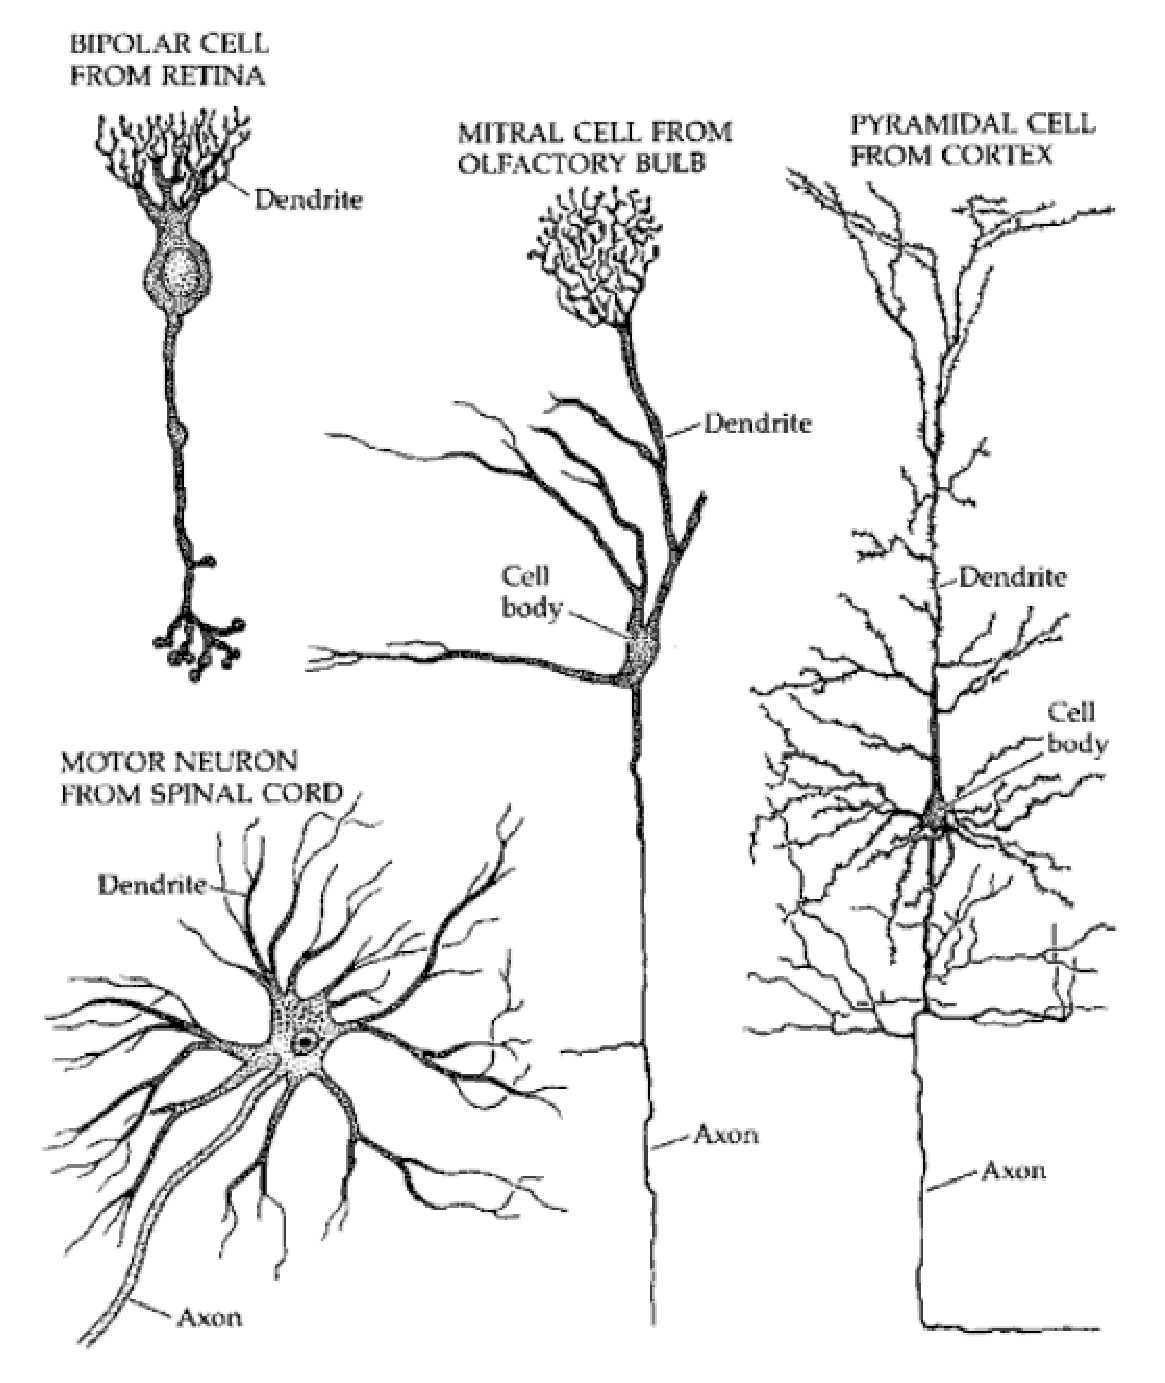
\includegraphics[height=8cm,
%     angle=0]{./images/neurons.eps}}
% \caption{Different morphologies of neurons}
% \label{fig:neurons}
% \end{figure}

% A neuron may receive input along its dendrites from a number of
% neurons, which is called {\bf convergence}, and transmit a signal
% along its axon to many other neurons, which is called {\bf
%   divergence}. The behavior of the dendrites, axon, and synapses are
% all quite different. 

% The electrical signal along the dendrites can be modeled as a passive
% process in which the diffusion of electricity is along a leaky cable,
% Chapter \ref{chap:dendrite-models}. The axon has an excitable membrane
% with different ion channels of the type described in
% Chapter~\ref{chap:voltage-gated-ionic}.
% The transmission of neurotransmitters at the synapse is described in
% Chapter \ref{chap:synapse-model-interc}. 


\subsection{Cylinder equivalent of dendritic tree}
\label{sec:cylind-equiv-dendr}

SUMMARY: We consider the ratio which is the sum of the $d^{3/2}$ of
the two branches divided by the $d^{3/2}$ of the parent branch. If
this ratio is idealized to 1 at every branch point, the entire
dendritic tree can be mapped to an equivalent cylinder,
Sec.~\ref{sec:unequal-branching}. Another requirement is that ``all
terminal branches terminate at the same electrotonic distance from the
soma''~\cite{rall2006bio}. However, the tree doesn't have to be
symmetrical, and the equivalent cylinder is valid not only for the
steady states, but also for transient solutions of the partial
differential equations~\cite{rall1962tpp}.  Rall introduced a new
variable $Z$ ({\bf electrotonic distance}), which is a generalization
of the variable $X=x/\lambda$ to the situation when the characteristic
length $\lambda$ is not constant. Aim: from

\begin{eqnarray}
  \label{eq:484}
      \frac{\partial V}{\partial T}  + V=
   \frac{\partial^2V}{\partial X^2} 
\end{eqnarray}
to 
\begin{eqnarray}
  \label{eq:483}
    \frac{\partial V}{\partial T} + V  =
   \frac{\partial^2V}{\partial Z^2} + K\frac{\partial V}{\partial T}
\end{eqnarray}

Despite the complexity of the geometry of neuron in a single cell, as
shown in Fig.~\ref{fig:neuron_cell}, it is assumed to be bounded by
one continuous membrane. A single neuron has 3 main parts: dendrite,
soma and axon.  The function of the soma-dendrite portion is to
receive and to integrate the signals from other cells. The signals can
be excitation and inhibition. When the resultant excitation signal
exceeds the threshold for ``action potential'' (key technical term),
then the axon will do its part, i.e. initiate a nerve impulse and
propagate it to the distant endings of this axon.  Thus, it's more
convenient to examine soma-dendrite and axonal portion in separate. In
this section we will focus on soma-dendrite portion.


Research works before 1956 mainly underestimated the importance of
dendrite to the receptive and integrative functions of the neuron. The
main reason was the wrongly belief that the density of synaptic
connections in dendrites is much less over that in soma membrane
surface. Nowadays, it is known that the density of synaptic
connections over the dendritic surface is as high as that over the
soma surface~\cite{rall1960mpt}, as shown in
Fig.~\ref{fig:synaptic_connection}.
 
\begin{figure}[hbt]
  \centerline{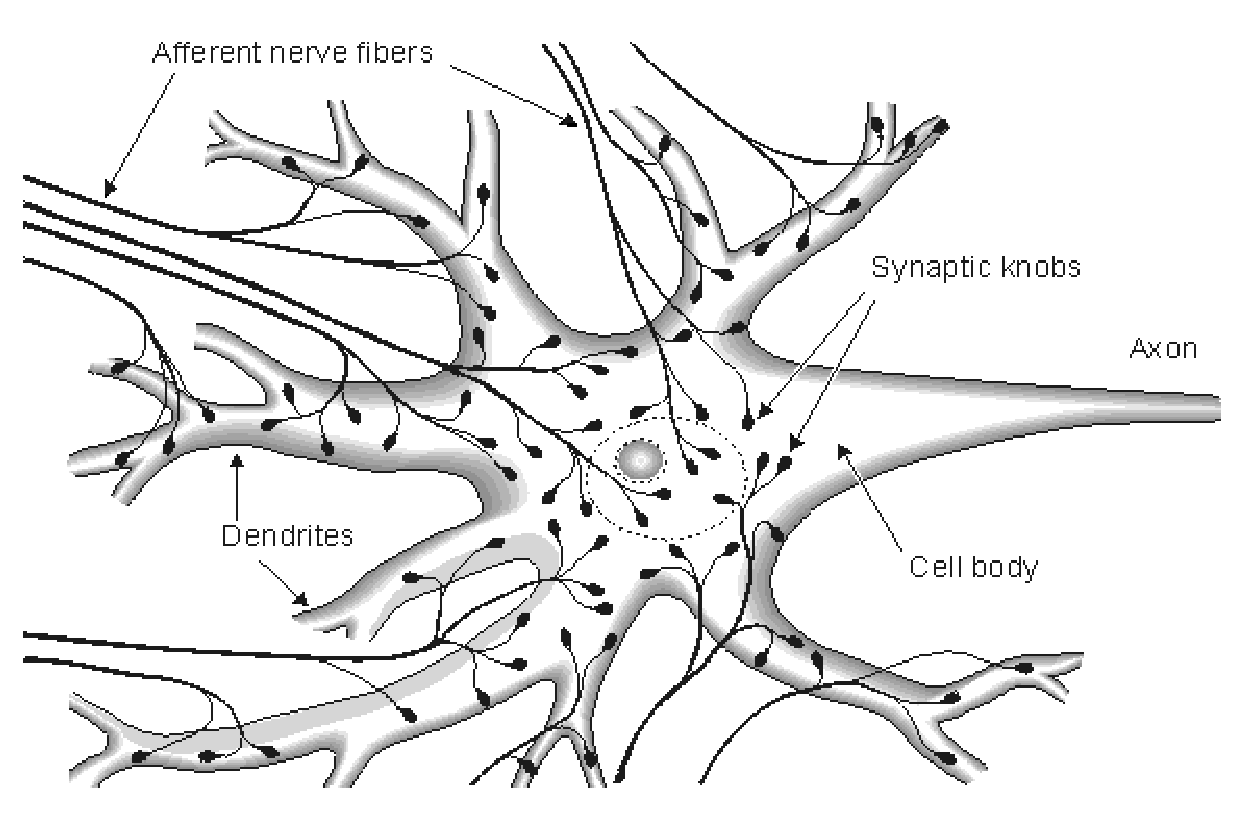
\includegraphics[height=6cm,
    angle=0]{./images/synaptic_connection.eps}}
\caption{Nerve ending connect to cortical nerve cell\footnote{\url{http://www.bem.fi/book/02/02.htm}}}
\label{fig:synaptic_connection}
\end{figure}


{\bf NOTE}: Dendritic trees of motoneurons have been found to
approximate the above conditions. 



\subsection{-- Equal branching}
\label{sec:equal-branching}

Based on the core-conductor model, we first consider a dendritic tree
defined by two functions of $x$: (1) the number of equal branches
present $n$ at any branching point of distance $x$ from the soma; (2)
the radius $r$ of these branches.

The internal axial dendritic current $I_i$ (mA), with $n$ branches of
equal radius $r$ can be expressed
\begin{eqnarray}
  \label{eq:482}
  I_i = \sum_{j=1}^n I_{i,j}= n \frac{1}{r_i}\left(-\frac{\partial
      V_i}{\partial x}\right) = (\pi r^2 n/R_i) \left( - \frac{\partial V_i}{\partial x} \right)
  % I_i = \sum_{j=1}^n I_{i,j}=(\pi r^2 n/R_i) \left( - \frac{\partial V_i}{\partial x} \right)
\end{eqnarray}
as $r_i = \frac{4R_i}{\pi d^2}$ with $d=2r$, and $R_i$ is the
intracellular specific resistivity (Ohm.cm), $V_i$ is the
intracellular electric potential, as shown in
Fig.~\ref{fig:current_i}.
\begin{figure}[hbt]
  \centerline{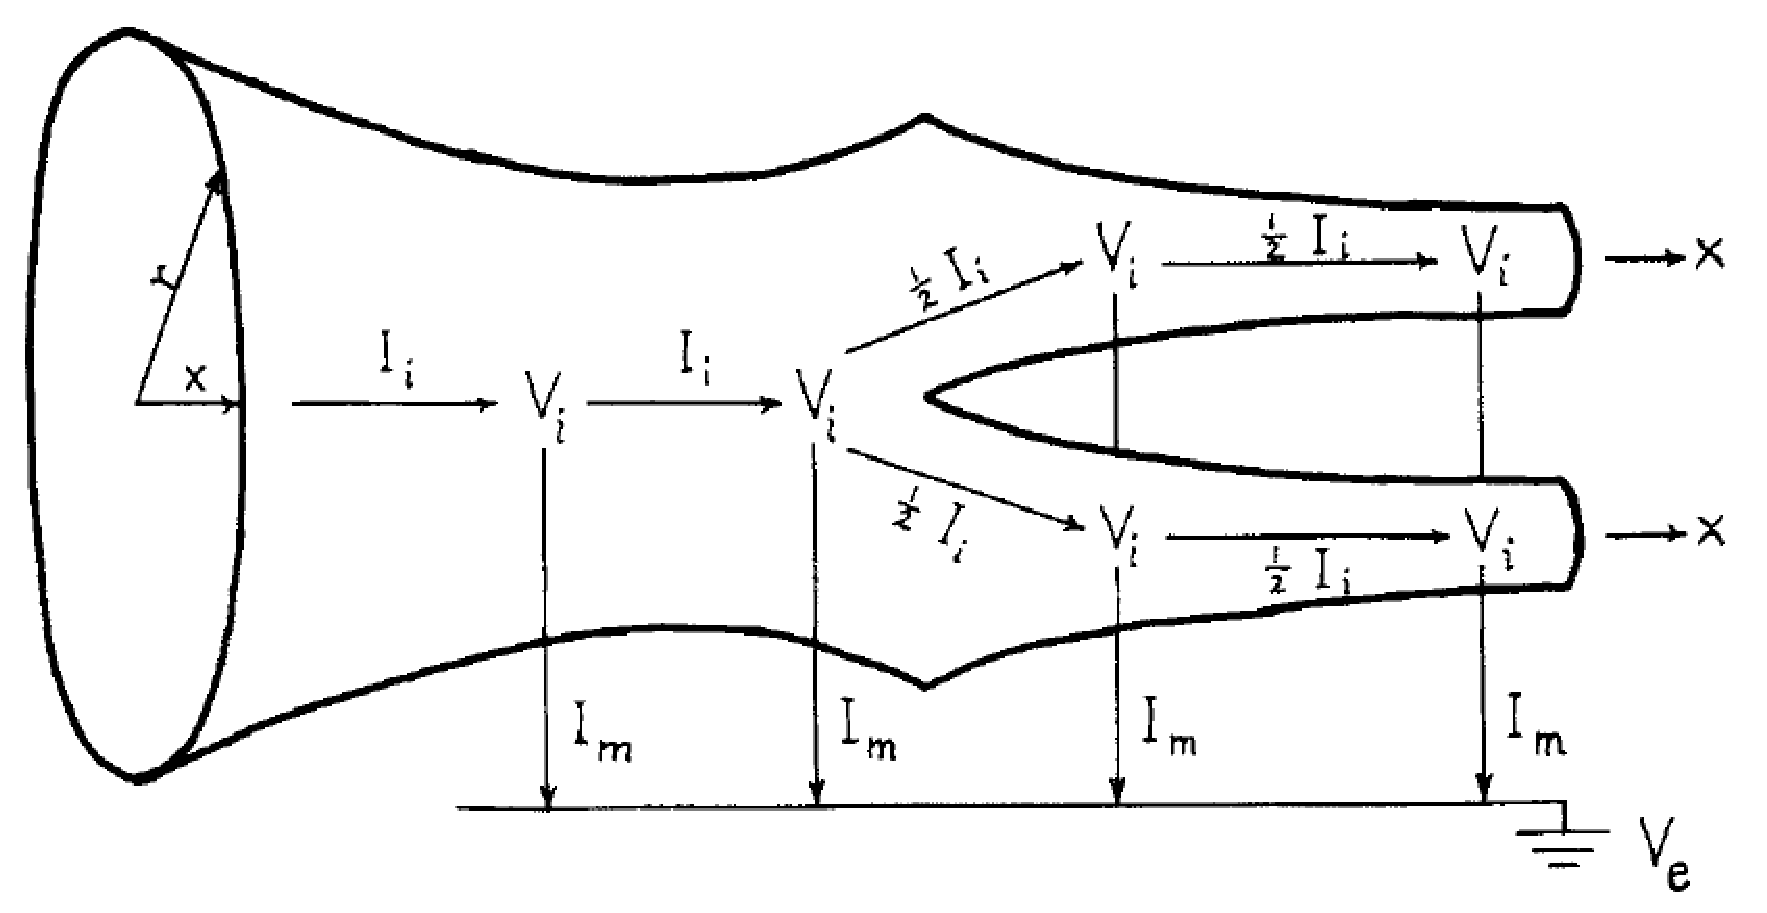
\includegraphics[height=5cm,
    angle=0]{./images/dendritic_branch.eps}}
\caption{Dendritic diagram showing $I_i$ (internal axial current),
  $V_i$ (intracellular potential), $I_m$ (membrane current density)}
\label{fig:current_i}
\end{figure}

As the current density is an area density (i.e. mA.cm$^{-2}$). Thus, % As $I=JA$ ($I$ is the current in the conductor, $J$ is the current
% density, $A$ is the cross-section area),
for points that are free of extracellular stimulus, the transmembrane
current density $I_m$ is
% equivalent to the decrease in internal current
% \begin{eqnarray}
%   \label{eq:486}
%   i_m = -\frac{\partial I_i}{\partial x}
% \end{eqnarray}
% then
\begin{eqnarray}
  \label{eq:513}
    I_m = \frac{I'}{A'}= -\frac{\partial I_i}{\partial x}\left[ \frac{dA}{dx}\right]^{-1}
\end{eqnarray}
with $dA$ is the dendritic surface area
\begin{eqnarray}
  \label{eq:488}
  \frac{dA}{dx} = 2\pi rn \frac{ds}{dx}
\end{eqnarray}

If there is taper of the dendritic branches, we have 
\begin{eqnarray}
  \label{eq:485}
  \frac{ds}{dx} = \left[ 1 + \left( \frac{dr}{dx}\right)^2 \right]^{1/2}
\end{eqnarray}
otherwise, we have $dr/dx = 0$, $ds/dx = 1$


To expand eq.~\eqref{eq:513}, we need to differentiate both sides of
eq.~\eqref{eq:482}
\begin{eqnarray}
  \label{eq:487}
  \frac{\partial I_i}{\partial x} &=& - (\pi r^2 n/R_i) 
    \frac{\partial^2V_i}{\partial x^2} - \pi/R_i \frac{\partial
      V_i}{\partial x} \frac{d}{dx}(r^2n) \\
    &=& - (\pi r^2 n/R_i) \left[
    \frac{\partial^2V_i}{\partial x^2} + \frac{\partial V_i}{\partial
      x} \frac{d}{dx}\ln(r^2n)\right]
\end{eqnarray}

Then,
\begin{eqnarray}
  \label{eq:435}
  I_m    &=& - (\pi r^2 n/R_i) \left[
    \frac{\partial^2V_i}{\partial x^2} + \frac{\partial V_i}{\partial
      x} \frac{d}{dx}\ln(r^2n)\right]
  \left[\frac{ds}{dx}\right]^{-1}\frac{1}{2\pi rn}\\ 
  &=& \frac{r}{2R_i} \left[\frac{ds}{dx}\right]^{-1} \left[
    \frac{\partial^2V_i}{\partial x^2} + \frac{\partial V_i}{\partial
      x} \frac{d}{dx}\ln(r^2n)\right]
\end{eqnarray}

Let's define a new variable $Z$ ({\bf electrotonic distance})
\begin{eqnarray}
  \label{eq:446}
  \frac{\partial V_i}{\partial x} = \frac{\partial V_i}{\partial Z} \frac{dZ}{dx}
\end{eqnarray}
then
\begin{eqnarray}
  \label{eq:497}
   \frac{\partial^2 V_i}{\partial x^2} &=& \frac{\partial^2 V_i}{\partial Z^2}
   \left[\frac{dZ}{dx}\right]^2 + \frac{\partial V_i}{\partial Z} \frac{d^2Z}{dx^2}
   \\
 &=& \left[\frac{dZ}{dx}\right]^2 \left( \frac{\partial^2 V_i}{\partial Z^2}
 + \frac{\partial V_i}{\partial Z}\left[\frac{dZ}{dx}\right]^{-1}
 \frac{\frac{d}{dx}\left(\frac{dZ}{dx}\right)}{\frac{dZ}{dx}}
\right)  \\
&=& \left[\frac{dZ}{dx}\right]^2 \left( \frac{\partial^2 V_i}{\partial Z^2}
 + \frac{\partial V_i}{\partial Z}\left[\frac{dZ}{dx}\right]^{-1}
 \frac{d}{dx}\ln\frac{dZ}{dx} \right)
\end{eqnarray}
Substitute back to eq.~\eqref{eq:435}, we have
\begin{equation}
  \label{eq:504}
  \begin{split}
    I_m &= \frac{r}{2R_i} \left[\frac{ds}{dx}\right]^{-1} \left[
      \left[\frac{dZ}{dx}\right]^2 \left(
        \frac{\partial^2 V_i}{\partial Z^2} +
        \frac{\partial V_i}{\partial Z}\left[\frac{dZ}{dx}\right]^{-1}
        \frac{d}{dx}\ln\frac{dZ}{dx} \right) +
      \frac{\partial V_i}{\partial
        Z} \frac{dZ}{dx} \frac{d}{dx}\ln(r^2n)\right] \\
    & = \frac{r}{2R_i} \left[\frac{ds}{dx}\right]^{-1} \left[
      \left[\frac{dZ}{dx}\right]^2 \frac{\partial^2 V_i}{\partial Z^2}
      + \frac{\partial V_i}{\partial Z}\left[\frac{dZ}{dx}\right]
      \frac{d}{dx}\ln\left( r^2n \frac{dZ}{dx} \right) \right] 
  \end{split}
\end{equation}
Then
\begin{equation}
  \label{eq:506}
  I_mR_m  = \frac{rR_m}{4R_i} \left[\frac{ds}{dx}\right]^{-1}
  \left[\frac{dZ}{dx}\right]^2 \left[ \frac{\partial^2
      V_i}{\partial
      Z^2}
    + \frac{\partial V_i}{\partial Z}\left[\frac{dZ}{dx}\right]^{-1}
    \frac{d}{dx}\ln\left( r^2n\frac{dZ}{dx} \right) \right]
\end{equation}


Now, $Z$ is defined to satisfy
\begin{eqnarray}
  \label{eq:505}
  \left[\frac{dZ}{dx}\right]= \left[\frac{rR_m}{2R_i}\right]^{-1/2} \left[\frac{ds}{dx}\right]^{1/2}
\end{eqnarray}
\textcolor{red}{When the cylindrical tree has no taper,
  $dZ/dx=\lambda$, thus $Z$ becomes $X$}.

The reduced form of eq.~\eqref{eq:506} is
\begin{equation}
  \label{eq:507}
  \begin{split}
    I_mR_m &= \frac{\partial^2 V_i}{\partial Z^2} +
    \frac{\partial V_i}{\partial Z}\left[\frac{dZ}{dx}\right]^{-1}
    \frac{d}{dx} \ln \left(
      r^2n\left(\frac{rR_m}{2R_i}\right)^{-1/2}\left(\frac{ds}{dx}\right)^{1/2}
    \right) \\
    &= \frac{\partial^2 V_i}{\partial Z^2} +
    \frac{\partial V_i}{\partial Z}\left[\frac{dZ}{dx}\right]^{-1}
    \frac{d}{dx} \ln \left( r^{3/2}n\left(\frac{ds}{dx}\right)^{1/2}
    \right)
  \end{split}
\end{equation}
as $\frac{R_m}{2R_i}$ is independent of $x$.

Interestingly, if
\begin{eqnarray}
  \label{eq:508}
  r^{3/2}n\left(\frac{ds}{dx}\right)^{1/2} = \text{constant}
\end{eqnarray}
then eq.~\eqref{eq:507} becomes
\begin{eqnarray}
  \label{eq:509}
  I_mR_m = \frac{\partial^2 V_i}{\partial Z^2} 
\end{eqnarray}

Dendritic trees satisfying eq.~\eqref{eq:508} (with K=0) is a subclass
of a larger class of dendritic tree whose branching satisfies
\begin{eqnarray}
  \label{eq:510}
  r^{3/2}n\left(\frac{ds}{dx}\right)^{1/2} = r_0^{3/2}n_0e^{K(Z-Z_0)}
\end{eqnarray}
with $r_0, n_0, Z_0$ are constants. If we consider the cylinder
starting from the soma, then $Z_0=0, n_0=1$ and $r_0$ is the trunk
radius. % is the radius of the parent cylinder, and $n_0$ is the
% number of branches at the parent level
$K$ is a constant. Under this condition, we have the new, compact form
of eq.~\eqref{eq:507}
\begin{eqnarray}
  \label{eq:511}
  I_mR_m = \frac{\partial^2 V_i}{\partial Z^2} +
 K \frac{\partial V_i}{\partial Z}
\end{eqnarray}
Under the subthreshold condition, i.e. passive nerve membrane, we have
\begin{eqnarray}
  \label{eq:512}
  I_mR_m=\Cm R_m\frac{\partial V_m}{\partial t}+V_m-E_r
\end{eqnarray}
Given that $V_m=V_i-V_e$, and $V=V_m-E_r=V_i-V_e-E_r$ ($E_r$ is the
resting potential). Under the condition that the extracellular medium
is isopotential, then $V_e=$constant; we also suppose $E_r=$constant
for all $r$ and $x$, then
\begin{eqnarray}
  \label{eq:515}
   I_mR_m = \frac{\partial^2 V}{\partial Z^2} +
 K \frac{\partial V}{\partial Z}
\end{eqnarray}
\textcolor{red}{Then
\begin{eqnarray}
  \label{eq:514}
  \frac{\partial^2 V}{\partial Z^2} +
  K \frac{\partial V}{\partial Z} = \frac{\partial V}{\partial T} + V
\end{eqnarray}
with $T=t/\tau$. The eq.~\eqref{eq:514} applies for all dendritic
trees whose branching satisfy eq.~\eqref{eq:510}. }

In summary, when $K=0$, the transformation of the variable $x$ to the
new variable $Z$ can be thought of as a transformation of a dendritic
tree into an equivalent cylinder with characteristic length $Z$. The
soma-dendritic system has been simplified to be modeled in terms of a
variable Z.

% % the increment of dendritic surface area to the increment in $x$
% At the points of branching, then $r$ and $n$ generally undergo finite
% discontinuities, then $ds/dx$ will be defined as unity at such points.



\subsection{-- Unequal branching}
\label{sec:unequal-branching}

The previous section assumes all branches are of equal radius with the
controlled function is eq.~\eqref{eq:510}. For unequal branches, we
replace the equation with a new condition
\begin{eqnarray}
  \label{eq:516}
  \sum_k \left[ \frac{r_k}{r_0}\right]^{3/2} = 1
\end{eqnarray}
The problem is very complicated when $K$ is not zero, or the impulse
approach a terminal boundary condition (i.e. non-linear behavior). 
That's why activities in the soma-dendritic system is always assumed
to be passive (subthreshold condition).


\subsection{-- Importances}
\label{sec:importances}

The equivalent cylinder is not of the same length as the branching
dendritic tree. A complete discussion of the cable theory for
dendritic tree can be reference with Rall (1989)~\cite{rall1989ctdn}.

\subsection{Models for dendritic membrane}
\label{sec:models-membrane}

\begin{figure}[hbt]
  \centerline{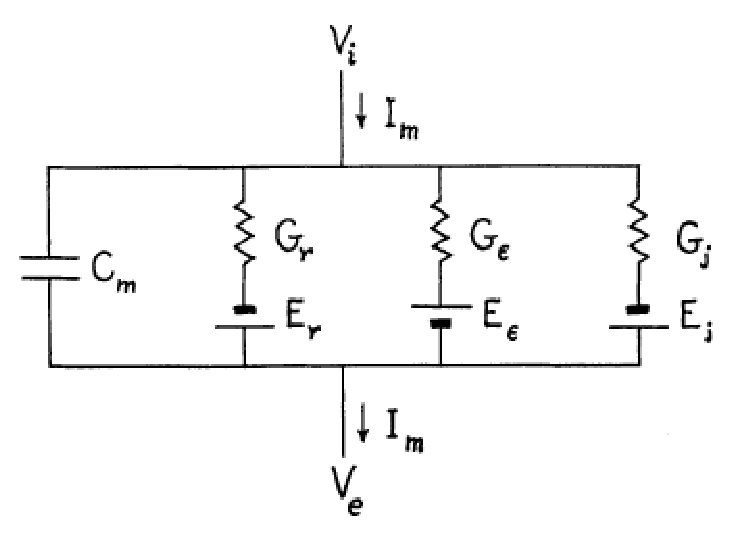
\includegraphics[height=5cm,
    angle=0]{./images/membrane.eps}}
 \caption{Diagram of electric model of nerve membrane}
\label{fig:membrane}
\end{figure}

A complete picture of the model is described with several parallel
electric pathway through the membrane: $\Cm $ (membrane capacity per
unit area), $G_r, G_\epsilon, G_j$ represent parallel conductance with
corresponding resting potential $E_r, E_\epsilon, E_j$ (the subscript
$r$ = resting membrane, $\epsilon$ = excitation, $j$ = inhibition).
\begin{enumerate}
\item The resting condition is obtained when $G_\epsilon = G_j = 0$. 
\item Synaptic excitation and inhibition will be treated as step
  increases of $G_\epsilon$ and $G_j$, respectively. 
\end{enumerate}
Based on the assumption, the membrane current density is given
\begin{eqnarray}
  \label{eq:520}
  I_m = \Cm  \frac{dV_m}{dt} + G_r(V_m-E_r) + G_\epsilon(V_m-E_\epsilon) + G_j(V_m-E_j)
\end{eqnarray}

Under the subthreshold condition, a passive membrane is modeled as an
impedance with $R_m$ in parallel with $\Cm $.
\begin{eqnarray}
  \label{eq:521}
  I_mR_m = \tau \frac{\partial V}{\partial t} + k^2(V-V^*)
\end{eqnarray}
with 
\begin{eqnarray}
  \label{eq:522}
  \tau &=& R_m\Csc  \\
  R_m &=& G_r^{-1}\\
  V &=& V_m-E_r \\
  k^2 &=& (G_r+G_\epsilon+G_j)/G_r \\
  V^* &=& \left[G_\epsilon(E_\epsilon-E_r) + G_j(E_j-E_r)\right] [k^2G_r]^{-1}
\end{eqnarray}
with $V^*$ represents the steady state value of $V$, $V$ represents
the departure from the resting potential $E_r$. 


\subsection[Boundary value problem]{Boundary value problem for
  membrane potential transient in dendritic trees}
\label{sec:bound-value-probl}

We treat the membrane potential transient in dendritic tree under the
condition\cite{rall1962tpp}
\begin{enumerate}
\item $K=0$
\item equal branching
\end{enumerate}

With $K=0$, we combine eq.~\eqref{eq:509} and eq.~\eqref{eq:521}, we
have
\begin{eqnarray}
  \label{eq:503}
  \frac{\partial^2 V_i}{\partial Z^2}  = k^2 (V-V^*) + \frac{\partial
    V}{\partial T}
\end{eqnarray}

The initial and boundary condition may be expressed as
\begin{eqnarray}
  \label{eq:524}
  V(Z,0) = f(Z)
\end{eqnarray}
with $\frac{\partial V}{\partial Z} = 0$, at $Z=0$ and $Z=L$. Using
Fourier series expansion, we can use
\begin{eqnarray}
  \label{eq:525}
  V(Z,T) = V^* + \sum_{n=0}^\infty C_n \cos(n\pi Z/L)e^{-\alpha_n^2T}
\end{eqnarray}
with
\begin{eqnarray}
  \label{eq:526}
  \alpha_n^2 &=& k^2 + (n\pi/L)^2 \\
  C_n &=& \frac{\int_0^L [f(Z)-V^*]\cos (n\pi Z/L) dZ}{\int_0^L
    \cos^2(n\pi Z/L) dZ}
\end{eqnarray}



\begin{figure}[hbt]
  \centerline{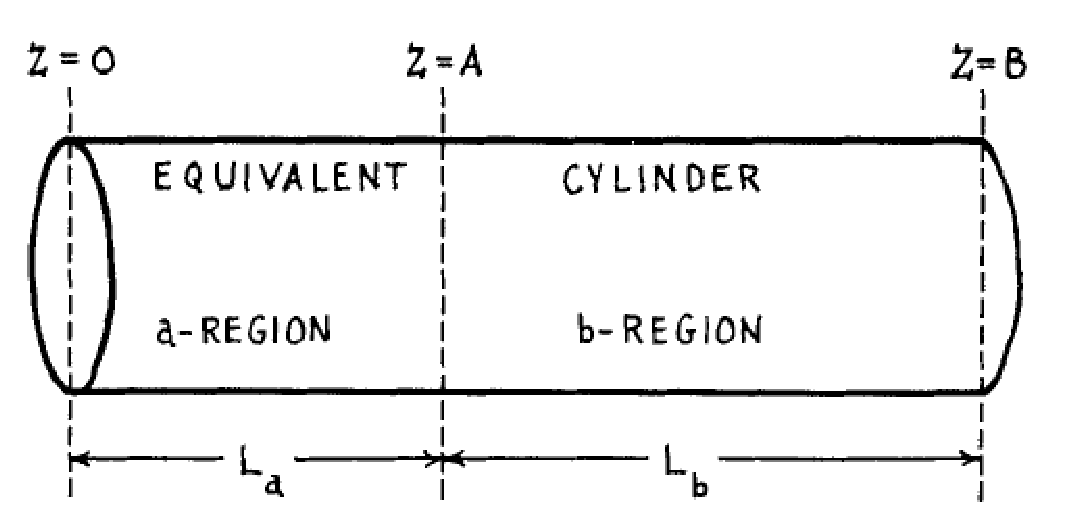
\includegraphics[height=5cm,
    angle=0]{./images/Z_cylinder_2.eps}}
\caption{An equivalent two-region cylinder}
\label{fig:two-region-cylinder}
\end{figure}

In the case that the electric parameters are not uniform over the
entire cylinder, we can divide it into segments. Suppose that the
cylinder is divided into two regions, with the electric parameters are
assumed to be uniform in each region, as shown in
Fig.~\ref{fig:two-region-cylinder}. Then the boundary condition 
\begin{itemize}
\item at a-region is $\frac{\partial V}{\partial Z} = 0$, at $Z=0$ and
  $Z=L_a$.

\item at b-region is (1) $\frac{\partial V}{\partial Z}= 0$ at $Z=0,
  Z=B$ and (2) the continuity of $V$ and $\frac{\partial
    V}{\partial Z}$ at Z=A.

\end{itemize}

Then the steady state solution of this boundary condition
is~\cite{rall1962tpp}
\begin{eqnarray}
  \label{eq:527}
  V(Z,0) &=& V_a^* + (V_A-V_a^*) \frac{\cosh(k_aZ)}{\cosh (k_aL_a)} \\
  V(Z,0) &=& V_b^* + (V_A-V_b^*) \frac{\cosh(k_b(B-Z))}{\cosh (k_bL_b)}
\end{eqnarray}
for $a-region$ and $b-region$, respectively.

The solution for the on-transient ($T>0$) $V(Z,T)$ is given
\begin{eqnarray}
  \label{eq:528}
  V(Z,T) = V(Z,\infty) + U(Z,T)
\end{eqnarray}
where
\begin{eqnarray}
  \label{eq:529}
  U(Z,T) &=& \sum_{n=1}^\infty D_n
  \frac{\cos(r_{an}Z)}{\cos(r_{an}L_a)}e^{-\gamma_n^2 T} \\
  U(Z,T) &=& \sum_{n=1}^\infty D_n
  \frac{\cos(r_{bn}Z)}{\cos(r_{bn}L_b)}e^{-\gamma_n^2 T}
\end{eqnarray}
for a-region and b-region, respectively. $\gamma_n^2$ are roots
(eigenvalues) of the characteristic function
\begin{eqnarray}
  \label{eq:530}
  r_{an}\tan(r_{an}L_a) = -r_{bn} \tan (r_{bn}L_b)
\end{eqnarray}
... (other parameters read the references)

An important property of the class of dendritic tree with $K=0$ is
that ``a constant increment $\Delta Z$, taken any where in the
dendritic tree correspond to a constant increment $\Delta A$ of
dendritic surface area''.
\begin{eqnarray}
  \label{eq:518}
  \frac{dA}{dx} \varpropto \frac{dZ}{dx}
\end{eqnarray}
Eq.~\eqref{eq:510} also implies
\begin{eqnarray}
  \label{eq:519}
  Z-Z_0 &=& \frac{1}{\lambda_0} \int_{x_0}^x
  \left[\frac{r_0}{r}\frac{ds}{dx}\right]^{1/2} dx \\
  &=& \frac{1}{\lambda_0} \int_{x_0}^x
  \left[\frac{n_0}{n}\right]^{1/3}\left[\frac{ds}{dx}\right]^{2/3} dx \\
\end{eqnarray}
when $K=0$. The initial increment $\Delta Z$, say $\Delta = 0.7$, of
each dendritic trunk is equivalent to the lumped soma, e.g. the soma
surface would represent $7\%$ of the total soma-dendritic surface
area.




\section{Numerical method unbranched cable equation: tridiagonal matrices}

% TODO: This section need to be disolved into PDE.tex somehow
Eq.\ref{eq:cable-equation} is rewritten
\begin{equation}
  \Csc \frac{\partial V_m}{\partial t} = \frac{d}{4R_i} \frac{\partial
  ^2V_m}{\partial x^2} - \sum_j G_{m,j} (V_m - E_j)  - I_\app
\end{equation}
with $j$ is the index of an ion type.

The second-order derivative is descritized using Euler-method into
\begin{equation}
\frac{\partial
  ^2V_m}{\partial x^2} = \frac{V_{i+1} - 2V_i + V_{i-1}}{\Delta x^2}
\end{equation}
then we have the equation 
\begin{equation}
  \Csc \frac{dV}{\Delta t} = \frac{d}{4R_i}
  \frac{V_{i+1}^{(t)} - 2V_i^{(t)} + V_{i-1}^{(t)}}{\Delta x^2} - \sum_j G_{m,j}
 \left( V_{i}^{(t)} - E_j \right)    - I_\app
\end{equation}
The index $i$ correspond to the locations along the cable (i.e. the nodes or
compartments). 

We will have one tridiagonal matrix + two diagonal matrices.
\begin{enumerate}
  \item diagonal matrices $\mathbf{C}^{-1}$ (inverse specific capacitance) and
  $\mathbf{G}$ (conductances)
  
  \item 
  A tridiagonal second-difference matrix with elements of (-2) along the diagonal
elements, and (+1) on both side
\begin{equation}
\mathbf{B'} = \left( 
\begin{array}{cccccc}
-2 &  1 & 0  & \ldots & 0 & 0 \\
1  & -2 & 1  &   &    & \\
0  &  1 & -2 & 1 & \ldots & 0\\
   &    &    &   &        & 0\\
   &    &    & 1 & -2 & 1 \\
   &    &    &   & 1 & -2 \\ 
\end{array}
\right)
\end{equation}
Other forms are also used: see Sect.\ref{sec:boundary-condition-cable-neuron}.
% \begin{equation}
% \mathbf{B'} = \left( 
% \begin{array}{cccccc}
% -2 & 1 & 0  & \ldots & 0 & \\
% 1 & -2 & 1 & & & \\
% 0 &  1 & -2 & 1 & \ldots & \\
%  & & & & & & \\
%  & & & 1 & 2 & 1 \\
%  & & & & 1 & -2 \\ 
% \end{array}
% \right)
% \end{equation}
  
\end{enumerate}

The matrix form of the cable equation:
\begin{equation}
\frac{d{\bf V}}{dt} = \mathbf{B.V} - \mathbf{I_\app}
\end{equation}
with 
\begin{equation}
\mathbf{B = C^{-1} \left( \psi B' - G\right)}
\end{equation}
with $\psi = \frac{d}{4 R_i \Delta x^2}$.

Due to the very strong coupling in voltage between two adjacent compartments, it
demands implicit  methods  (Sect.\ref{sec:implicit-method}) for  numerical
stability with reasonable time steps  and  therefore a  matrix  equation  must 
be  solved  every  time  step (Sect.\ref{sec:solve-oder}).

\begin{mdframed}

Solving a linear cable of $n$ compartments (indeed $n+2$ with two compartments
at two ends as the boundary condition) can be organized in the form of
tridiagonal matrix, in which the membrane potential at compartment $i$ is at
$A(i,i)$, and its calculation is based on two neighboring $A(i-1,i)$ and
$A(i,i+1)$, in which 
\begin{itemize}
  \item $A(i-1,i)$ mirrors the value of $A(i,i)$
  \item $A(i,i+1)$ mirrors the value of $A(i+1,i+1)$
\end{itemize}
so that $A(i-1,i-1)$ and $A(i+1,i+1)$ can be updated in parallel with $A(i,i)$.

\end{mdframed}

\subsection{Solving nonlinear equation using Picard iteration}
\label{sec:iteration-solving-nonlinear-equation}
\label{sec:Picard-iteration}

Suppose you have the equation of voltage solved by implicit methods; and the
gates as well

\begin{verbatim}
// voltage makes use of values of m,n,h
B . V(t+dt)_{i-1}  - D . V(t+dt)_i + A . V(t+dt)_{i+1} = C . V(t) - gamma_{t+dt}

//m, n, h gates
m(t+dt) - m(t) / dt = a_m(V(t+dt)) (1 - m(t+dt)) - b_m(V(t+dt)).m(t+dt)  
\end{verbatim}

Since these equations coupled through the future and unknown value
\verb!V(t+dt)!, they needs to be solved simultaneously. 

One way to solve such system is using Picard iteration
\begin{enumerate}
  \item prediction step 1:  
  
  solve voltage at time (t+dt), using V(t) and gates (m,n,h) at times
  (t)
  
  \item predict step 2: update m,n,h using the predicted value v(t+dt)
  
  \item correct step 1:
  
   solve voltage again at time (t+dt), using V(t) and gates (m,n,h) at times
  (t+dt)
  
  \item correct step 2: 
  
It is possible to stop at here.
Since backward Euler is first order in time anyway, a simpler approach is to update
the voltage and the gating variables only once instead of using Picard iteration

  
  \item returns to step 2 untils Vm and gates are converged
\end{enumerate} 

\subsection{dV/dt: forward Euler}
\label{sec:forward-Euler}

The question is when the derivative \verb!f(V)! is estimated?
\begin{verbatim}
dV/dt =  f(V,t)
\end{verbatim}
\begin{enumerate}
  \item In forward Euler method: the derivative is estimated at time t
  
\begin{verbatim}
[ V(t+dt) - V(t) ]/dt = f(V(t), t)
\end{verbatim}
or
\begin{equation}
V(t+dt) = f(V(t), t) * dt + V(t)
\end{equation}
\end{enumerate}

\begin{equation}
  \Csc \frac{V_i^{(t+\Delta t)} - V_i^{(t)}}{\Delta t} = \frac{d}{4R_i}
  \frac{V_{i+1}^{(t)} - 2V_i^{(t)} + V_{i-1}^{(t)}}{\Delta x^2} - \sum_j G_{m,j}
 \left( V_{i}^{(t)} - E_j \right)    - I_\app
\end{equation}

COST: 3 multiplications per node (one for itself, two for communicating with
two adjacent nodes).

A new matrix form can be used
\begin{equation}
\mathbf{V}^{(t+\Delta t)} = \mathbf{B}_f \mathbf{V}^{(t)} - \mathbf{I_\app}
\end{equation}
the left-hand side is a column-vector, and the tridiagonal matrix
\begin{equation}
\mathbf{B}_f = \mathbf{I} + \Delta t \mathbf{B}
\end{equation}

CONS: The method is unstable if $\Delta t$ is too large, i.e. condition for
stability
\begin{equation}
\Delta t \le \frac{R_i \Csc \Delta x^2}{d}
\end{equation}
It means that to achieve the same stability, and if you want to increase 2x the
spatial discretization, i.e. double the matrix size, the time step must be made
4x smaller than the time step in the previous setting. 
Since doubling the spatial discretization step also doubles the size of the matrix,
computation time scales as the third power of $n$.


\subsection{dV/dt: implicit (backward) Euler}
\label{sec:implicit-method}
\label{sec:backward-Euler}

The question is when the derivative \verb!f(V)! is estimated?
\begin{verbatim}
dV/dt =  f(V,t)
\end{verbatim}
\begin{enumerate}
 \item In backward Euler method: the derivative is estimated at time (t+dt)
 which improves numerical stability
  
\begin{verbatim}
[ V(t+dt) - V(t) ]/dt = f(V(t+dt), t+dt)
\end{verbatim}
or
\begin{equation}
V(t+dt) = f(V(t+dt), t+dt) * dt + V(t)
\end{equation}

The equation is derived from Taylor's series truncated at the $\Delta t$ term
but with $t + \Delta t$ in place of t.

\end{enumerate}

For the cable equation (Sect.\ref{sec:cable-equation-discritize}), we have
\begin{equation}
\begin{split}
  \Csc \frac{V_i^{(t+\Delta t)} - V_i^{(t)}}{\Delta t} = \\
  & \frac{d}{4R_i}
  \frac{V_{i+1}^{(t + \Delta t)} - 2V_i^{(t + \Delta t)} + V_{i-1}^{(t + \Delta
  t)}}{\Delta x^2} \\
  & - i_m (V_i^{(t+\Delta t)}) + i_\app
\end{split}
\end{equation}
 this solution depends on the current at a future time, which we will have to
approximate. 

or
\begin{equation}
\begin{split}
  \Csc \frac{V_i^{(t+\Delta t)} - V_i^{(t)}}{\Delta t} = \\
  & \frac{d}{4R_i}
  \frac{V_{i+1}^{(t + \Delta t)} - 2V_i^{(t + \Delta t)} + V_{i-1}^{(t + \Delta
  t)}}{\Delta x^2} \\
  &- \sum_j G_{m,j} \left( V_{i}^{(t + \Delta t)} - E_j
  \right)    - I_\app
\end{split}
\end{equation}

PROS: The implicit scheme is stable for all time step.

CONST: It comes at a cost of finding the inverse of a $n\times n$ matrix 
$\mathbf{B}_b = \left[ \mathbf{I} - \Delta \mathbf{B} \right]^{-1}$ which is
$\bigO(n^3)$ - the same cost as the explicit method.

SOLVE:
\begin{equation}
\mathbf{V}^{(t + \Delta t)} = \mathbf{B}_b \mathbf{V}^{(t)}
\end{equation}

Note: Picard iteration is an option to solve - Sect.\ref{sec:Picard-iteration}.

\subsection{dV/dt: semi-implicit (Crank-Nicolson or central-difference method)}
\label{sec:Crank-Nicolson-method}

The Crank-NiCholson method (Crank and Nicholson 1947), is
equivalent to advancing by one half step using backward Euler and then advancing
by one half step using forward Euler.
\begin{itemize}
  \item first compute V(t+dt/2)
  \item then simply apply
  
\begin{verbatim}
V(t+dt) = 2 * V(t+dt/2) - V(t)
\end{verbatim}
\end{itemize}
So, the extra accuracy does not cost extra computations
of the model functions.

Cooley and Dodge (1966) organized the compartments in a cable into sparse
symmetric matrix, and then using Crank-Nicolson
(Sect.\ref{sec:Crank-Nicolson-method}) for the diffusion term and an iterative
procedure for the nonlinear reaction term - the first time a second-order
numerical method was demonstrated for the Hodgkin-Huxley equations.

Later, in 1984, Hines developed an improved method with 3 improvements
(Sect.\ref{sec:Hines-matrix}) which can result in a 10–20-fold decrease in
computation time for simulation of arbitrarily branched active cables with
Hodgkin Huxley (HH) kinetics.

\begin{equation}
\begin{split}
  &\Csc \frac{V_i^{(t+\Delta t)} - V_i^{(t)}}{\Delta t} = \\
  &\frac{d}{4R_i}
  \frac{ \frac{1}{2} \left( V_{i+1}^{(t)} + V_{i+1}^{(t + \Delta t)} \right) -
  2\frac{1}{2} \left( V_i^{(t)} + V_i^{(t + \Delta t)} \right) + 
  \frac{1}{2} \left( V_{i-1}^{(t)} + V_{i-1}^{(t +
  \Delta t)} \right) }{\Delta x^2} \\
  &- \sum_j G_{m,j} \left(
  \frac{1}{2}\left( V_{i}^{(t)} + V_{i}^{(t + \Delta t)}\right) - E_j \right)   
  - \frac{I_{\app,i}^{(t)} + I_{\app,i}^{(t+\Delta t)}}{2}
\end{split}
\end{equation}

PROS: stable for all choices of discretization. It is more preferable to the
implicit method (as it is more accurate with second-order in time).


\subsection{dV/dt: Crank-Nicolson-Hines}
\label{sec:Crank-Nicolson-Hines}

The original Crank-Nicholson method can produce artifactual large amplitude
oscillations if the time step is too large. This can affect simulations of
models that involve voltage clamps or in which adjacent segments are coupled by
very small resistances.

NOTE: When \verb!secondorder=2! is used (Sect.\ref{sec:fadvance-NEURON}), this
variant method, known as Hines-Crank-Nicholson is used in NEURON.
\begin{itemize}
  
  \item NOTE: In implicit integration methods, \textcolor{red}{all current
  balance equations must be solved simultaneously}. However, it is not easy to
  solve non-linear function of conductance; which typically requires iterations
  
Nonlinear equations generally need to be solved iteratively to maintain second
order correctness.

However, voltage dependent membrane properties, which are typically formulated
in analogy to Hodgkin-Huxley (HH) type channels, allow the cable equation to be
cast in a linear form, still second order correct, that can be solved without
iterations.

  \item use of a staggered time step algorithm to avoid iteration of nonlinear
  equations, i.e. 
\begin{itemize}
  \item voltage is computed at time v(t), v(t+dt)
  \item state variables are computed at time v(t-dt/2), v(t+dt/2)
\end{itemize}
So the requirement becomes \textcolor{red}{ only the
solution of simultaneous linear equations.}

Here, HH type channels are easy to solve at t + dt/2 since the conductance is
a function of state variables which can be computed using a separate time step
that is offset by dt/2 with respect to the voltage equation time step.

Since the current balance equations have the structure of a tree (there are no
current loops), direct gaussian elimination is optimal for their solution (Hines
1984)


  \item
\end{itemize}

Hines modified the Crank-Nicolson method by applying it in two consecutive time
step of $\Delta t/2$. So, instead of using a single equation with time-step
$\Delta t$, two stages method is used, each with time-step $\Delta t/2$.

\begin{equation}
\begin{split}
  &\Csc \frac{V_i^{(t+\Delta t/2)} - V_i^{(t)}}{\Delta t/2} = \\
  &\frac{d}{4R_i}
  \frac{ V_{i+1}^{(t + \Delta t/2)} -
  2 \left( V_i^{(t)} + V_i^{(t + \Delta t/2)} \right) + 
  \frac{1}{2} \left( V_{i-1}^{(t)} + V_{i-1}^{(t +
  \Delta t/2)} \right) }{\Delta x^2} \\
  &- \sum_j G_{m,j} \left(
  \frac{1}{2}
  \left( V_{i}^{(t)} + V_{i}^{(t + \Delta t/2)}\right) - E_j \right)   
  - I_{\app,i}^{(t+\Delta t/2)}
\end{split}
\end{equation}

Having solved voltage at $V_i^{t+\Delta t/2}$, and with $V_i^{t}$, an explicit
step is used to find voltage at $(t+\Delta t)$
\begin{equation}
V_i^{t+\Delta t} = 2 * V_i^{t+\Delta t/2} - V_i^{t}
\end{equation}

\subsection{Rempe-Chopp (2006) - nonlinear gating variable}
\label{sec:Rempe-Chopp-2006}

If the dimensionless variable $(m,n,h)$ as gating variables are known at time
$(t+\Delta t/2)$, then they can be used directly in estimating 
$V^{t+\Delta t/2}$ in a conditionally linear system (a property proposed by
Mascagni and Sherman).  This is similar to Crank-Nicolson-Hines method
(Sect.\ref{sec:Crank-Nicolson-Hines}).

The final ingredient needed to make sure the method is second order in time is a
second-order accurate method updating the gating variables. So
\begin{equation}
\begin{split}
\frac{dm}{dt} &= \alpha(\Vm)- (\alpha(\Vm) + \beta(\Vm)) m \\
 &= \alpha(\Vm) \times (1-m) - \beta(\Vm) \times m
\end{split}
\end{equation}
can be solved using
\begin{equation}
\frac{m^{t+\Delta t/2} - m^{t - \Delta t/2}}{\Delta t} = 
\alpha(\Vm^{t})-
(\alpha(\Vm^{t}) + \beta(\Vm^{t})) m^{t} 
\end{equation}

As we don't have $m^{t}$, it can be approximated using
$m^{t} = \frac{m^{t+\Delta t/2}+m^{t-\Delta t/2}}{2}$.

Finally
\begin{equation}
\begin{split}
m^{t+\Delta t/2} &= \frac{\alpha}{\frac{1}{\Delta t} + \frac{1}{2} (\alpha
+\beta)} + \left( \frac{\frac{1}{\Delta t} - \frac{1}{2} (\alpha
+\beta)}{\frac{1}{\Delta t} + \frac{1}{2} (\alpha
+\beta)} \right) m^{t-\Delta t/2}  \\
  &= \frac{\alpha \Delta t}{1 + \frac{\Delta t}{2} (\alpha
+\beta)} + \left( \frac{1 - \frac{\Delta t}{2} (\alpha
+\beta)}{1 + \frac{\Delta t}{2} (\alpha
+\beta)} \right) m^{t-\Delta t/2}
\end{split}
\end{equation}

NOTE: If we consider the effect of temperature via Q10, then 
$\Delta t$ is replaced by $(\Delta t \times \Phi)$ with $\Phi$(Q10) is
calculated using Sect.\ref{sec:q10-factor}.


\subsection{Discritize cable equation}
\label{sec:cable-equation-discritize}

\begin{equation}
\Csc \frac{\partial V}{\partial t} = \frac{a}{2 R_a} \frac{\partial^2
V}{\partial x^2} - i_m(V) + i_\app
\end{equation}
with $\Csc$ (specific membrane capacitance: F/cm$^2$ or $\muF$/cm$^2$); V
(transmembrane potential: mV); $a$ (radius of cable/segment: cm or $\mum$); 
$R_a$ (cytoplasmic resistivity: $\Omega.$cm); $i_m(V)$ (all transmembrane
current from either active or passive processes).

\url{http://jneuron.readthedocs.io/en/latest/Theory.html}

Suppose a segment of length $\Delta x$; we can discritize the second-order
part into
\begin{equation}
\Csc \frac{\partial V}{\partial t} = \frac{a}{2 R_a} \frac{V_{i+1} -
2 V_i + V_{i-1}}{\Delta x^2} - i_m(V) + i_\app
\end{equation}

As the cable equation is not an ODE (Sect.\ref{sec:ode}), but a parabolic
partial differential equation, the solution is going to be more tedious and
idiosyncratic to the problem.

The main points are that we need to maintain some desired level of accuracy, be
it first order or second order; and we need to consider the stability of our solution. 
When using implicit methods (e.g. Sect.\ref{sec:backward-Euler},
Sect.\ref{sec:Crank-Nicolson-method}), solution for time t=t1 depends on some
values at t=t2 in the future. As you would expect, we will need to employ some
trickery to approximate the values we need at t=t2, since we haven't solved for that time
yet.  


For the current
\begin{equation}
i_m (V_i(t+\Delta t)) = i_m (V_i(t)) + \Delta V_i \frac{di_m}{dV_i}
\end{equation}
Where we can approximate the instanenous conductance in our simulation by
evaluating the current at the known voltage and then at v=v+.001. In other
words, $\Delta V_i = 0.001$ (mV).

Convert to matrix math (as we need to solve for many segments (i.e.
compartments) in one section or many section, i.e. branch)
\begin{enumerate}
  
  \item Everything on the right-hand-side (RHS) of the equation
  \begin{itemize}
    \item the (axial) current density entering a given segment from the parent
    segment
    \item the (axial) current density(s) leaving the given segment to its child
    segments
    
    \item the membrane current due to activate and passive components at the
    current time step can all be calculated during a given iteration.
  \end{itemize}
  
  \item On the left-hand-side (LHS) of the equation
  \begin{itemize}
    \item every coefficient of the  $\Delta V$  terms are constant with the
    exception of the $di_{m,i}/dV$ term which changes from iteration to
    iteration.
  \end{itemize}
  
  \item  At every iteration then, we calculate that right hand term for each
  segment, calculate di/dv for each segment and add it to the diagonal term, and
  then solve for $\Delta V$ by simple matrix math.

 Therefore, the most efficient way to simultaneously solve for the change in
voltage at all of the segments would be to calculate the constant coefficients
for the left hand side, which will complete a matrix, A, relating the change in
voltage at one node to the change in voltage at another.  

At every iteration then, we calculate that right hand term for each segment,
calculate di/dv for each segment and add it to the diagonal term.


\end{enumerate}

\subsection{Boundary condition}
\label{sec:boundary-condition-cable-neuron}

When a cell is modeled as a cable, we need two boundary conditions, one at each
end of the cable. However, there are many physical condition that the boundary
condition can be at the point in the middle, e.g. voltage is clamped to zero or
the axial currents leak to the ground.

{\bf OPTION 1}:
\textcolor{red}{Programmingly, we need to add border to the matrix {\bf B'}}
(and thus {\bf B}), so that we can treat boundary condition properly
(Sect.\ref{sec:boundary-condition}).
\begin{enumerate}
  \item killed-end (Dirichlet condition): leaky at ends (as $V_{stencil}=0$)
  \item sealed-end (von Neumann condition): no flux (as $dV/dt = 0$)
\end{enumerate}
The left-side boundary is saved on the first (stencil) row of the matrix
$\mathbf{B}$.
The right-side boundary is saved on the last (stencil) row of the matrix.

Situation with one or two ends ``leaky'' are considered by
Rall (Sect.~\ref{sec:boundary-condition}). Cables with sealed ends are described
by Traub et al.~\citep{traub1991nnh} (page 78-83).

{\bf OPTION 2}:  with sealed-end condition, we can assume the loss at two end is
half of the other nodes in the middle, so a new tridiagonal matrix is used (not
the value -1 at two ends)
\begin{equation}
\mathbf{B'} = \left( 
\begin{array}{cccccc}
-1 & 1 & 0  & \ldots & 0 & \\
1 & -2 & 1 & & & 0 \\
0 &  1 & -2 & 1 & \ldots & 0\\
 & &  & & & 0\\
 & & & 1 & -2 & 1 \\
 & & & & 1 & -1 \\ 
\end{array}
\right)
\end{equation}
IMPORTANT: This approximation is only correct in first-order 
$\bigO(\Delta x)$.
This implementation introduces a systematic error or phantom currents (Niebur
and Niebur, 1991).

{\bf OPTION 3}: a more accurate scheme that give second-order correct sealed-end
condition
\begin{equation}
\mathbf{B'} = \left( 
\begin{array}{cccccc}
-2 & 2 & 0  & \ldots & 0 & \\
1 & -2 & 1 & & & 0\\
0 &  1 & -2 & 1 & \ldots & 0\\
 & &  & & &  0\\
 & & & 1 & -2 & 1 \\
 & & & & 2 & -2 \\ 
\end{array}
\right)
\end{equation}

\subsection{Number of elements in a tridiagonal matrix}

A $n \times n$ matrix has $3n-2$ non-zero elements.

\subsection{Solving order}
\label{sec:solve-oder}

\begin{enumerate}
  \item hodgkin-huxley ionic channels: 
  $I_{HH}(V_m(x,t),t)$ = $\sum_j G_{m,j}(V_m - E_j)$
  
  \item find the tridiagonal matrix
  
  \item solve the final voltage 

Suppose the intermediate has been computed, then it takes $\bigO(n)$ to solve
the column-vector $\mathbf{V}$, using Gaussian elimination thanks to the
sparseness of the tridiagonal matrices on the right-hand side.
\end{enumerate}


\section{Branching model of dendrites}
\label{sec:model-dendrite}

\subsection{simple treatment}

NOTE: Based on the cable equation (eq.\ref{eq:cable-equation}), here we also
consider the effect of synaptic current contributions (which is treated
differently than ionic currents)
\begin{equation}
\Csc \frac{dV_m}{dt} = \frac{d}{4R_i} \frac{\partial^2 V_m}{\partial
x^2} -I_\ion - I_\app - I_\synaptic
\end{equation}

\subsection{advanced treatment}

As we have two time of taking the spatial derivative, some methods use different
values of $a(x,t)$, so they split $a(x,t)$ into the first and second order
derivative, each will get a different value (example: see
Sect.\ref{sec:kozloski2011-NTS})
% \begin{equation}
% \Csc \frac{\partial V_m(x,t)}{\partial t} = \text{RHS}(V_m) +
% \frac{d}{4R_i} \frac{\partial^2 V_m}{\partial x^2}
% \end{equation}
\begin{equation}
\label{eq:cable-equation-spatial}
\begin{split}
\Csc \frac{\partial V_m(x,t)}{\partial t} &= 
\frac{1}{2\pi a(x)} \frac{\partial}{\partial x}\left( \frac{\pi a^2(x)}{R_i}
\frac{\partial V_m}{\partial x} \right)
- G_i (V_m - E_i) - I_\app - I_\synaptic   \\
&= \frac{1}{2\pi a(x)} \frac{\partial}{\partial x}\left( \frac{\pi a^2(x)}{R_i}
\frac{\partial V_m}{\partial x} \right)
- \sum G_i \times V_m + \text{RHS}(E_i)
\end{split}
\end{equation}


with $\text{RHS}({V_m}) = \sum G_i \times E_i - I_\app$ represents
the part that can be calculated without using $V_m$
(RHS = right-hand side), and $d=2\times a(x)$.

NOTE: For a single compartment of length $\Delta x$, the total capacitance 
$\Cm$
and total axial resitance $R$ are
\begin{equation}
\begin{split}
\Cm &= \Csc \times \pi \times d \times \Delta x \\
R &= R_i \times \frac{\Delta x \times 4}{\pi \times d^2}
\end{split}
\end{equation}
so $\frac{1}{R} = \frac{\pi \times a^2}{R_i}\frac{1}{\Delta x}$.

So, by multiplying $2\pi \times \Delta x \times a(x)$ to both sides of
eq.\ref{eq:cable-equation-spatial}, we have the equation that takes into account
compartment side (length + radius)
\begin{equation}
\begin{split}
\Cm \frac{\partial V_m(x,t)}{\partial t} 
&= \Delta x \frac{\partial}{\partial x}\left(
\frac{\Delta x}{R} \frac{\partial V_m}{\partial x} \right) \\
&+ (2 \pi \times \Delta x \times
a(x) ) 
\times \sum G_i . V_m(x,t) + (2\pi \times \Delta x \times
a(x)) \text{RHS}(E_i) 
\end{split}
\end{equation}


At a branch-point, a conservation of charge requires
\begin{equation}
\frac{1}{A}\sum \frac{\pi a^2}{R_i}\frac{\partial V_m}{\partial x} = \Csc
\frac{\partial }{\partial t} + I_\total
\end{equation}
with $I_\total = I_\ion + I_\synaptic + I_\app$ (the sume of currents through
ion channels, synaptic currents, and any externally applied currents).

\subsection{Hines algorithm (solve branched dendrites)}
\label{sec:model-dendrite-branching-Hines-algorithm}

Here; the whole  neuron is organized in a single linear system of matrices.
Each matrix element represents a compartment. As a single linear system, optimal
solution of the tree matrix via Gaussian elimination is normally  accomplished 
by  a  recursive,  and  therefore serial,  algorithm.

To help solving the voltage at all nodes in a branched dendrites in $\bigO(n)$
using Gaussian elimination, \citep{hines1984} implemented a numerical scheme,
originally proposed by Cooley and Dodge (1966) for organizing the nodes in a
branching dendrite into sparse symmetric matrix (Sect.\ref{sec:Hines-matrix}),
and then using Crank-Nicolson (Sect.\ref{sec:Crank-Nicolson-method}) for the
diffusion term and an iterative procedure for the nonlinear reaction term - the
first time a second-order numerical method was demonstrated for the
Hodgkin-Huxley equations.


% Rather than providing a single equation that approxiate the branched dendrite 
% like Rall's method (Sect.\ref{sec:model-dendrite_cable-approximation
% -of-branching})
\url{http://neuroinf.blogspot.com/2014/04/from-pdes-to-hines-solver.html}

\begin{mdframed}

Remember: $\frac{dy}{dt}_k = -y^2_k$, with time $t=[0,a]$; the system is
discritized into $n$ time-steps of $\Delta t = \frac{a}{n}$.
[notation: $y_k = y(t_k)$]. Both forward and backward Euler methods have
$O(\Delta t)$ accuracy.

\begin{enumerate}
  \item forward Euler explicit scheme: $\frac{y_{k_1}-y_k}{\Delta t}= y^2_{k}$
  
\begin{equation*}
y_{k+1} = y_k - \Delta t y^2_k
\end{equation*}

  \item backward Euler implicit scheme: 
  $\frac{y_{k_1}-y_k}{\Delta t}= y^2_{k+1}$ (a quadratic function of the future value)

\begin{equation*}
y_{k+1} = \frac{-1 + \sqrt{1 + 4\Delta t y_k}}{2\Delta t}
\end{equation*}

\textcolor{red}{IMPORTANT}: In the vast majority of cases, the equation to be
solved when using an implicit scheme is much more complicated than a quadratic
equation, and no analytical solution exists.

\end{enumerate}

\end{mdframed}

The dendritic branch is spatially descritized into a set of connected
compartments, so from a single equation
\begin{equation}
\frac{\partial V}{\partial t} + I_\ion(V,t) = \frac{\partial^2 V}{\partial x^2}
\end{equation}
which is a PDE w.r.t space and time. 
We want to convert to first-order derative
in time, by converting into a set of ODEs; and then an implicit integration method is used to solve the time-evolution of membrane
voltage (Hines, 1984) - Sect.\ref{sec:NEURON-implicit-methods} (Reference:
Sect.\ref{sec:model-dendrite}).

Under \textcolor{red}{2 main assumptions (approximations)}:
\begin{enumerate}
  \item axial current is specified in terms of voltage drop between the centers
  of the two connected compartments
  
  So, the smaller the compartment the more precised the calculation
  
  \item spatially varying membrane current is represented by its value at the
  center of each compartment
\end{enumerate}
If \textcolor{red}{all compartments are of equal size}, the above approximations
each has error proportional to the square of compartment length, the
second-order partial derivative is approximated by its central different
approximation, which introduces an error proportional to $\Delta x^2$, and it
produces a family of ODEs
\begin{equation}
c_j \frac{dv_j}{dt } + i_{\ion_j} = \sum_k \left( \frac{v_k -
v_j}{r_{jk}}\right) + i_\stim
\end{equation}
with $j$ is the index of $j$-th compartment. Based on Kirchhoff's current law,
the net transmembrane current leaving the $j$-th compartment must equal to the
sum of all axial current entering the compartment from all sources (i.e. all
connected branches).
\begin{itemize}
  \item $r_{jk}$ = the resistance between 2 compartments $j$ and $k$
  \item $i_{\ion_j}$ = all ionic currents across the membrane of $j-$th
  compartment
  \item NOTICE the subtraction from neighboring compartments $v_k$ to the
  current one, indicate the influx of current (which of course can be positive
  or negative)
\end{itemize}
Sign convention: outward transmembrane current = positive, axial current flow
into a region= positive.

IMPORTANT: Based upon the above analysis, doubling the number of compartment
reduces the error by a factor of 4. 

If the compartments are of unequal size, the rough rule of thumb is that
simulaton error is proportional to the square of the size of the largest
compartment.

\textcolor{red}{\bf Capacitance of a cylinder (compartment)} of diameter $d$ and
length $\Delta x$: the capacitance is 
\begin{equation}
\Csc \times \pi \times d \times \Delta
x
\end{equation}
and the axial resistance is 
\begin{equation}
R_a \times \frac{\Delta x}{\pi (d/2)^2} 
\end{equation}
with $\Csc = 1 \muF/\cm^2$; the axial resistivity $R_a$ (Sect.\ref{sec:axial-current})

A {\bf section} maps to a morphological part of the neuron, and each section can
be represented by one or many connected compartments of equal length. For
each segment, the number of compartments is specified via \verb!nseg!. To help
defining value that varies depending on the position over the length of the
section (e.g. distribution of some ionic channels via the increasing of
conductance over the length), the values in relative to the position is
specified in terms of normalized distance \verb!x! (from 0 (proximalEnd) to 1
(distalEnd)). It makes it easier to describe the properties of each section
without regarded to the number of segments used to represent it.

A {\bf node} associates with one section, and defines the voltage of the
segment. The nodes of two adjacent sections are linked (connected) by resisters.
The location of the center of one node is defined as
\begin{verbatim}
x = (2 * i - 1)/ (2*nseg)
\end{verbatim}
with $i$ integer in the range [1,nseg]. \verb!x! is used
to retrieve the state variables that are a function of position along a section.

\subsection{* Hines matrix}
\label{sec:Hines-matrix}

In the matrix form of a single cable, the nodes are organized in the
order of their physical relation along the cable. In a branching dendritic tree,
this make it harder to solve the system.

Hines developed a numering scheme, using depth-first search or breadth-first
search that rearrange the order of the different segments that help to create a
symmetric matrix that can be solved efficiently.

\begin{mdframed}
A matrix {\bf H} is Hines matrix if it satisfies 3 conditions:
\begin{enumerate}
  \item diagonal elments are non-zero: $H(i,i) \ne 0$
  \item $H(i,j)$ is non-zero if and only if $H(j,i)$ is non-zero
  \item for any non-zero $H(i,j)$ with $i<j$ (i.e. above the diagonal line),
  there is no other non-zero elements $H(i,h)$ with $h>j$. This guarantees there
  are maximum three non-zero elements on a each row.
\end{enumerate}

There are many Hine matrices that can be derived from a tree structure.
\end{mdframed}

\begin{equation}
\mathbf{H . V}^{(t+1)} = \mathbf{V}^{(t)}
\end{equation}

The matrix is tridiagonal, except at points correspond to branching. Initially,
the whole neuron branching tree is treated as a single matrix
(single linear system to be solved) \citep{hines1984}.
Later, a neuron splitting scheme was used that allows solving different
branching trees from the same soma in parallel using a
fully implicit method
(Sect.\ref{sec:NEURON-implicit-methods}) \citep{hines2008fip}.

The matrix $\mathbf{A}$ represents voltage from a set of branch segments in an
arbor that need to be solved in a single phase.

\subsection{* Boundary condition at end-points (junction points)}




\subsection{* Implicit methods}
\label{sec:NEURON-implicit-methods}

Using one of the two stable {\bf implicit methods}
\begin{enumerate}
  \item backward Euler: a numerical error is proportional to $\Delta t$
  
  can be used with large time step to find steady-state solution for linear
  (passive) system.
  
  \item variant of Crank-Nicolson method
  (Sect.\ref{sec:Crank-Nicolson-method}):
  a numerical error is proportional to $\Delta t^2$
  
  can be used when small time-step is required, by setting the global parameter 
  \verb!secondorder=2!.
\end{enumerate}

Here, all current balance equations are solved simultaneously

Hine's algorithm performs Crank-Nicolson into 2 separate steps of
time-step $(\Delta t/2)$ (Sect.\ref{sec:Crank-Nicolson-Hines})
\begin{verbatim}
predict()      
               find Vm at time (t+dt/2)
update_Vm      
              use an explicit formula
              V(t+dt) = 2* V(t+dt/2) - V(t)               
\end{verbatim}



\subsection{Cai et al. (1997)}

\citep{cai1997} proposed a similar branch-numbering procedure like Hines
(1984) (Sect.\ref{sec:model-dendrite-branching-Hines-algorithm}) to update the
voltage of the tree in O(N) operations.

\subsection{Hines-2008 version (splitting into multiple matrices)}

The neuron can have multiple dendritic trees, and Hines method in 1984 organized
into a single tridiagonal matrix, i.e. a single linear system for the entire
neuron (Sect.\ref{sec:model-dendrite-branching-Hines-algorithm}).

\citep{hines2008nsc} developed a newer version that enables subtrees that
originate at the same neuron root can be solved in parallel, i.e. multiple
linear systems in which each system represents a single dendritic subtree.
This is called {\it neuron splitting techniques} and has now been extended
to take many forms. Any  compartment  can  serve  as  the  root  of
the tree, yet typically the soma compartment is chosen as the root.

The fully implicit approach by Hines et al. yields a stable and accurate
solution at the level of the neuron, even when neurons are coupled via chemical
synapses, but can not be extended to include electrical synapses. In tissues
containing electrical synapse,  Hines' approach must be modified to include
explicit terms everywhere electrical synapses occur.

The introduction of explicit terms and fixed-point iteration to solve for
electrical synapses limits the stability and accuracy of the overall numerical
method, however.

These explicit terms occur wherever electrical synapses occur, rather than at
specific, well- defined locations like junctions, such that their numerical
effects may be difficult to control.

The method of Rempe-Chop is good, but it doesn't use the implicit method
which is critical when ``{\it very strong coupling between adjacent compartment
voltages demands implicit methods for numerical stability with reasonable time
steps}'', as stated by Hines \citep{hines2008fip}.

Surprisingly however, Rempe-Chop were able to show empirically that their method
was sufficiently stable and accurate to permit the use of reasonable time-step,
upto 100$\mus$.

\subsection{Mascagni (1991) - multiple linear systems}
\label{sec:Mascagni-1991}

\citep{mascagni1991} decomposed the single neuron into multiple linear systems,
each for a single branch structure. 
These linear systems are tridiagonal, so the computational cost for updating one
branch is O(N) operations, where N is the number of compartments in that branch.

For each branch the principle of superposition is employed to construct the
solution as the sum of two or three solutions to linear systems for that branch.
However, the superposition approach requires an additional solution of a dense
linear system corresponding to the voltage at the branch points, which couples
all the branches together, and consequently the evolution on the whole cell is
again required.

\subsection{-- solving}

A system is ``Conditional linearity'' and full second-order accuracy in time
if values of data (e.g. gating variables $m,h, n, \ldots$) are known at offset
time-steps, i.e. that is $V_m$ is calculated at $t, t+\Delta t, t + 2\Delta
t$,\ldots and gating variables are calculated at times $t+\Delta t/2$, 
$t+(3\Delta t/2)$, 
 $t + (5\Delta t/2)$, \ldots
 
\begin{verbatim}
findgating
              find data at time (t+dt/2)
              using a second-order accurate method
              (trapezoidal rule)
predict()      
               find Vm at time (t+dt/2)
               using data at time (t+dt/2)
update_Vm      
              use an explicit formula
              V(t+dt) = 2* V(t+dt/2) - V(t)
                             
\end{verbatim}


Trapezoidal rule is used to update the values at offset times: for $m$ gating
variable, for example
\begin{equation}
\frac{m^{t+\Delta t/2} - m^{t-\Delta t/2}}{\Delta t}
= \alpha_m(V^t) - (\alpha_m(V^t) +\beta_m(V^t)) 
\frac{m^{t+\Delta t/2} + m^{t-\Delta t/2}}{2}
\end{equation}
or an equivalent formula
\def\tp{{\text{tp}}}
\begin{equation}
m^{t+\Delta t/2} = \frac{\alpha_m + \left(  1 - \tp \right)m^{t-\Delta
t/2}}{1+\tp}
\end{equation}
with $\tp$ can be
\begin{equation}
\tp = \frac{\Delta t}{2} (\alpha_m + \beta_m)
\end{equation}
or, if the temperature adjustment is considered, with $\Phi$
(Sect.\ref{sec:q10-factor}), then
\begin{equation}
\tp = \frac{\Delta t}{2} (\alpha_m + \beta_m) \times \Phi
\end{equation}



\subsection{Rempe-Chopp algorithm - multiple linear systems (cut at
branch-point, use explicit method)}
\label{sec:Rempe-Chopp}

\citep{rempe2006} decomposed the whole neuron branching trees into implicitly
solved branches (similar to that of Mascagni (1991) -
Sect.\ref{sec:Mascagni-1991}), yet avoid using the dense linear system - hence
making it easier for parallelization, i.e. the so-called {\bf spatial
adaptivity}. Spatial adaptivity within the tree structure is a novel development
in neural simulations.

Each branch is completely uncoupled from the other branches. Branches
are updated only if they are active and turned off as they return to the equilibrium
resting voltage, and introduced an explicit
predictor-corrector scheme for the membrane potential at branch points.

\subsection{-- cut phase}

In Hines (2008), the whole tree is splitted at a single point - the so-called
'root' compartment. Here, multiple linear systems are derived, from multiple
nodal points. Nodal points are chosen as points at which branching occurs.

So, in a single neuron, we can have $N_b$ branches and $N_n$ nodal points. 
A nodal points couple two or more branches through the branch's one of the
two end points, $B_{i^\pm_j}$ (the $\pm$ indicates whether index=0 (the first
compartment) or index=size-1 (the last compartment) on that branch).

\subsection{-- matrix of the end-points}

The voltage matrix of the branch points, which couples all the branches
together, can be a dense linear system, i.e. when each branch point links to so
many branches.



\subsection{-- solving backward Euler predictor-corrector}

This is first-order of accuracy in time. Here it uses Picard iteration


\begin{verbatim}
   branch-i         branch-(i+1)       branch-(i+2)     timestep
 data-array        data-array
---------------|-----------------|----------
 predict ()       predict ()          predict ()          dt        explicit
 forwardsolve     forwardsolve        forwardsolve
 correct ()       correct ()          correct ()
 backwardsolve    backwardsolve       backwardsolve
         syncdata              syncdata
\end{verbatim}

\begin{verbatim}
predict_step() 	       predict Vm at time-step (t+1) using 
                       data (m,h,n,Vm) at
                       time-step (t)
                       and explicit method
forwardSolve()                        
                       update data (m,h,n) 
                       using Vm just calculated as the boundary condition

correctStep()                        
                       correct Vm at time-step (t+1)
                       using the just updated data
                       and implicit-like method
backwardSolve()                       
                       update data (m,h,n) again using
                       the corrected Vm                      
syncdata 
                       exchange end point data between nodes
\end{verbatim}

\subsection{-- solving: Crank-Nicolson predictor-corrector}

There are two stages: forward-time calculation (i.e. predictor) and then
backward-time calculation (i.e. corrector) - both utilize implicit methods.
An explicit step is used to predict the value of the membrane potential at the
branch point at the forward time.

% \begin{verbatim}
%    branch-i         branch-(i+1)       branch-(i+2)
%  data-array        data-array
% ---------------|-----------------|----------
%         predict_step()      predict_step()
%  forwardsolve     forwardsolve        forwardsolve
%         correct()           correct()
%  backwardsolve    backwardsolve       backwardsolve
% \end{verbatim}
% 
% The \verb!predict_step()! on branch-i provides a prediction of the voltage
% (i.e. just copy the last element) value on the first element of the Vm[] array
% on the branch-(i+1) which is used in \verb!forwardsolve()! step on branch-(i+1).
% 
% Once all branches complete their \verb!forwardsolve()!, then a new value of the
% voltage on the first element of the Vm[] array on the branch-(i+1) is used to
% updated (corrected) the last element of the Vm[] array on the branch-i.
% 
% A \verb!backwardsolve()! is done on every branch, to complete one iteration.



{\bf REMARKS}:
This approach effectively decouples the solution of the membrane potential
between branches, permitting an implicit scheme within each branch.
{\it Hines' large linear system is thus replaced with a set of {\bf much
smaller} linear systems that are {\bf truly tridiagonal} and decoupled from each
other, and can therefore be solved efficiently and simultaneously in parallel
within a single neuron.}




\subsection{Kozloski (2011) (treat all cuts (at branch-point, at the middle of a
branch) as junction-point)}
\label{sec:kozloski2011-NTS}

\citep{kozloski2011}: A neuron is decomposed into branches, branch points, and
somata, which in turn are decomposed into compartments. Branches comprise one or
more compartments, while branch points and somata correspond to a single
compartment each.
A typical neuron has about O(1000) branch compartments, each is described by two
spherical endpoints (x,y,z,r).
The somata and branch point compartments are then described by single spheres
within this scheme.

The cut points in the previous methods are at branching points, i.e. each
linear system represents the whole branch.
\textcolor{red}{Here, the cut points are determined at any location within a
branch at which it intersects with a slicing plane}
(Sect.\ref{sec:kozloski2011-slicing-plane}).
This, nevertheless, the cut point can also coincide with a branching point.

If the slicing plane cut through a compartment, the compartment is then assigned
to the volume containing the compartment's proximal endpoint (except for branch
points, which are assigned to the same volume as their proximal compartment) and
initialized on the machine node assigned their volume. \textcolor{red}{How
about synapses} (Sect.\ref{sec:kozloski2011-synapse}).
% TODO: Idea, here, we should keeps the branching point for easier solving ???
%      So, at an intersection with a slicing plane, the nearest branch-point is
% used


As a result, branches whose compartments were assigned to more than one volume
are effectively cut into multiple branches. So, a single branch of $N$
compartments can be represented by two linear systems (we call it a 'capsule' -
Sect.\ref{sec:kozloski2011-capsule}), each one has $N_1$ and $N_2$ compartments
respectively, and $N = N_1 + N_2$ (and the slicing plane cuts through the
compartment $N_1$, using 1-based index).

\begin{mdframed}
So, we are solving not a the branch-level, but at capsule-level.
To facilitate the communication between two 'capsules', which can occurs on 2
different computing nodes with separate memory spaces, a Proxy instance is also
generated. 

The NTS is responsible for initializing branches and junctions, and their
proxies, in order to ensure that the Model Graph Simulator's collective
communication is consistent and matched across all volume boundaries (node-node
pairs).

In terms of computational performance, it is best if two nodes solving two sets
of adjacents capsules are computational-'adjacent' to each other.
In theory, for Blue Gene/P, link bandwidth is maximum between nearest neighbors
and measures 6.8 GB/s, while bisection bandwidth varies between 1.7 and 3.8
TB/s, depending on the machine size.

\end{mdframed}

The cut point is called a JunctionPoint in this scheme. Of course, we also need
the EndPoint in each compartment.

 Now consider a fully implicit parallel solver that replaces all explicit
junctions between branches with implicit junctions 

All branches of a particular branch order (defined neuroanatomically as the
number of junctions between the branch and the soma) are computed within a
single phase.

\subsection{-- initiation}

Sect.\ref{sec:NTS_simulation}.

\subsection{Branches + BranchPoint}



\subsection{-- max compute order}
\label{sec:kozloski2011-capsule}

The decomposition of a neuron into implicitly solved tree partitions
(capsules) separated by explicit junctions. 

The tuning parameter (\verb!maximum compute order!), a trade off occurs between
the numerical stability and accuracy of the combined method, and the efficient
parallel execution of the computational algorithm that implements it.

\subsection{-- solving}



\begin{verbatim}
   branch-i         branch-(i+1)       branch-(i+2)
 data-array        data-array
---------------|-----------------|----------
 calPlasticity   calPlasticity        calPlasticity
 solveChannels   solveChannels        solveChannels
        predictJunction()      predictJunction()
 forwardsolve7     forwardsolve7        forwardsolve7
 forwardsolve6     forwardsolve6        forwardsolve6
  ...
 forwardsolve1     forwardsolve1        forwardsolve1 
 solve             solve                solve 
 backwardsolve1     backwardsolve1        backwardsolve1
 ...
 backwardsolve6     backwardsolve6        backwardsolve6
 backwardsolve7     backwardsolve7        backwardsolve7 
        correctJunction()       correctJunction()
  finish            finish               finish
\end{verbatim}


\subsection{- choice of slicing planes}
\label{sec:kozloski2011-slicing-plane}

The slicing plane is the plane splitting two cubic volume
- each volume represent the computing works for a single node.

Slicing planes are chosen to accomplish a weighted histogram equalization of
compartments across slices in each of the three-dimensions of slicing. Weights
for each compartment are calculated based on a sum of weights of its associated
channel and branch models.

These weights were determined experimentally and reflect the expected
computational load of each model.

\subsection{-- synapse}
\label{sec:kozloski2011-synapse}

A synapse is treated as a simple neuron, with two compartment: 
\begin{itemize}
  \item 'soma' compartment for 'pre-synapse' region
  \item one-compartment apical-dendrite for 'post-synapse' region.
  % TODO: we may need to split post-synapse region into head + neack
  
  \textcolor{red}{TUAN: How about splitting two regions: head + neck}
\end{itemize}

Synapses are also initialized within the volumes containing their presynaptic
and postsynaptic compartments.



\section{Model dendritic spines}



Recently, with the evidence of dendritic spines
(Sect.\ref{sec:dendritic_spines}) in synaptic plasticity, new approaches have
been proposed. The first approach was called the {\bf continuum theory} or the
new cable theory (Sect.\ref{sec:new-cable-theory}). 
A simpler one is the {\bf Spike-Diffuse-Spike model}
(Sect.\ref{sec:spike-diffuse-spike-model}.


\subsection{New cable theory (continuum model)}
\label{sec:new-cable-theory}
\label{sec:dendritic_spines_model}

It's only until recently that we can study the electrical properties of
dendritic spines (Sect.\ref{sec:dendritic_spines}) thanks to recent advances in
imaging technologies as well as the use of two-photon glutamate uncaging. We
suspects that there are voltage-dependent \ce{Na+}, \ce{K+}, and \ce{Ca^2+}
channels in the spine heads.

Using cable theory, the spine is modeled as two compartments: one for
the head and one for the neck connecting the spine head to the
dendrite. The compartment representing the head should carries active
properties. 

One of the novel model is {\bf Baer and Rinzel's continuum model}
\citep{baer1991}.  
%\subsubsection{Baer-Rinzel (continuum model) - 1991}
Baer-Rinzel proposed a new cable theory for which the distribution of
dendritic spine is treated as continuum \citep{baer1991}, which was recently
review by Baer \cite{baer2014}.

The formulation maintains the feature that there is no direct electrical
coupling between neighboring spines; voltage spread along dendrites is the only
way for spines to interact.

\subsection{Spike-diffuse-spike (SDS) model}
\label{sec:spike-diffuse-spike-model}

SDS model is a computationally simple version of the full Baer and Rinzel model
\citep{coombes2000}.
The model drops the continuum approximation and instead uses a passive dendrite
coupled to excitable spines at discrete points.
The spike events are modelled in a discrete fashion with the wave form
conventionally represented as a rectangular function.

It reduced the number of free parameters, and retain those of greatest
significance, such as spine neck resistance.
 

References:
\begin{itemize}
\item \url{http://en.wikipedia.org/wiki/Dendritic_spine}
\end{itemize}


% At some point along the cylinder, the voltage $V_m$ is the function of
% both time and distance from the injected point. Thus
% \begin{eqnarray*}
%   \frac{\partial V_m}{\partial x} = -r_i I_i
% \end{eqnarray*}
% The negative sign means the voltage decrease when increasing $x$.  The
% leak current $I_m$ across the membrane (through $r_m$ and $\Cm$) is
% equal to the decrease in $I_i$. Thus
% \begin{eqnarray*}
%   \frac{\partial I_i}{\partial x}=-I_m
% \end{eqnarray*}
% The current across the membrane $I_m$ is the combination of current
% across the capacitor and ionic channels, thus
% \begin{eqnarray*}
%   i_m = i_C + i_{ionic} = \Cm\frac{\partial V_m}{\partial t} + \frac{V_m}{r_m}
% \end{eqnarray*}
% Finally,
% \begin{eqnarray}
%   \label{eq:4081}
% \frac{1}{r_i}  \frac{\partial^2 V_m}{\partial x^2} = \Cm\frac{\partial V_m}{\partial t} + \frac{V_m}{r_m}
% \end{eqnarray}
% % or
% % \begin{eqnarray}
% %   \label{eq:409}
% %   \Cm\frac{\partial V_m}{\partial t} + \frac{V_m}{r_m}  
% % \end{eqnarray}
% This is also known as the {\bf cable equation}, derived form the
% one-dimensional cylinder. 

% Another form of the cable equation is
% \begin{eqnarray}
%   \label{eq:410}
% \lambda^2 \frac{1}{r_i}  \frac{\partial^2 V_m}{\partial x^2}  =
% \tau_m \Cm\frac{\partial V_m}{\partial t} + V_m
% \end{eqnarray}
% with $\lambda$ is called the {\bf space constant} (or {\bf length
%   constant}). 
% \begin{eqnarray*}
%   \lambda = \sqrt{\frac{r_m}{r_i}} = \frac{aR_m}{2*R_i}
% \end{eqnarray*}
% If we need to include the extracellular resistance, then $\lambda =
% \sqrt{\frac{r_m}{r_i+r_o}}$.
% $\tau_m=r_mc_m=R_m\Cm$ is the membrane time constant. 



% Current $I_\app $ injected into the membrane will flow both along the
% cylinder $I_i$ (x-direction only) and across the membrane $I_m$. Thus,
% using the Kirchoff's law, the equation is
% \begin{eqnarray*}
%   I_\app  = I_i + I_m
% \end{eqnarray*}

%\subsection{Branching in the dendrite}


\subsection{Modeling spine $\Ca$ transients}
\label{sec:spine-model-with-Ca-transient}

Calcium transients in spines are a key trigger for synaptic plasticity
\citep{nevian2006}.


There are evidence that spine head shrink momentarily in response to Ca2+ influx
\citep{korkotian2001}, which decrease spine head volume about 10\% and may cause
instantaneous intra-spine pressure. The significiance of this twitch is not
know, as they appears to be more pronounced in idle spines.

\section{Model a nerve cell}
\label{sec:model-cell}

The three major questions:
\begin{enumerate}
  \item One of the first question to answer is the passive electrical features along the
dendrites, independent of synaptic inputs and voltage-dependent channels.
  \item Second is how to describe synaptic input. 
  \item And the third one is how to
  simulate voltage-dependent and calcium-dependent current. 
\end{enumerate}

The early works tried to answer the first one, i.e. subthreshold condition where
no action potential is generated (Sect.\ref{sec:electrotonus_vs_transient}).
Because of the small diameter of the axon (i.e. high input impedance), the
effect of the axon on subthreshold condition is neglected. Thus, we mainly deal
with the soma and dendrite. The soma is approximated by a sphere, while the
dendrite is modeled as a cable of non-isopotential membrane. Then, the cable
theory was developed for long dendrite or axon (Sect.\ref{sec:non-isop-cell})
where the propagation along the cable is passive.


% The electrical signal along the dendrites can be modeled as a passive
% process in which the diffusion of electricity is along a leaky cable,
% Chapter \ref{chap:dendrite-models}. The axon has an excitable membrane
% with different ion channels of the type described in
% Chapter~\ref{chap:voltage-gated-ionic}.
% The transmission of neurotransmitters at the synapse is described in
% Chapter \ref{chap:synapse-model-interc}. 


\begin{framed}

As there is not a single type of neurons, with a given model for one neuronal
type to match the experimental data of different types of neurons, the model may
need to change only the value of the membrane time constant $\tau_m$; others may
need to change the values of theoretical parameters corresponding to
electrotonic length (electrotonic distance) or to time course of synaptic
current; or some require explicit consideration of several dendrites (e.g. basal
and apical dendrites of pyramidal neurons). We will discover them from simple to
complicated.
\end{framed}



\cite{finn2002hnm}Cable theory was first presented by William Thompson
(later Sir.Kelvin) in 1855 when he studied the electrical propagation
of the signals in the submarine telegraph cables. This theory applies
for signal transmission on a single spatial dimension and describes
both steady-state and transient solution for particular boundary
condition and initial conditions.  The theory was further developed
for neurons by Hermann in 1870s~\cite{hermann1879hdp}.

The continuous form of the cable model was derived from a compartment
model that consists of a series of compartments, each with a
resistance and a capacitance. 
\begin{itemize}
\item each compartment represent a segment of the cell with a length
  $\Delta x$.
\begin{figure}[hbt]
 \centerline{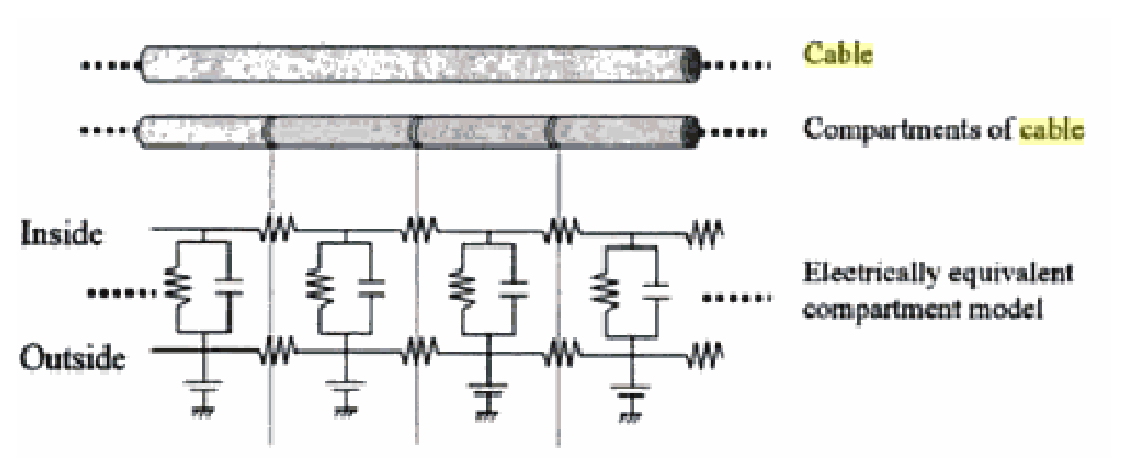
\includegraphics[height=5cm, angle=0]{./images/compartment_model.eps}}
\caption{Compartment model of a cable. The transmembrane resistance is
model as a resistance in parallel with capacitance.}
\label{fig:compartment_model}
\end{figure}

\item the cable equation is derived for each individual compartment
  using Kirchoff's law
\begin{figure}[hbt]
 \centerline{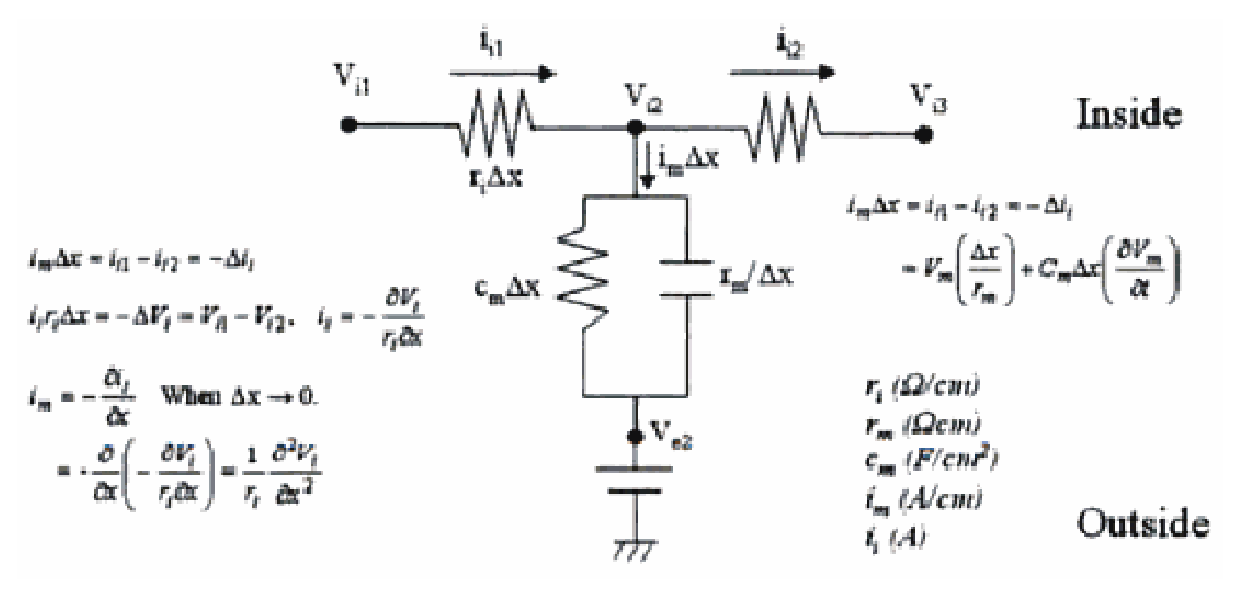
\includegraphics[height=5cm, angle=0]{./images/cable_equation.eps}}
\caption{Application of Kirchoff's current law}
\label{fig:cable_equation}
\end{figure}

\end{itemize}


\section{Boundary condition}
\label{sec:boundary-condition}

To determine the behavior of a single dendrite, we need an initial
condition (voltage at time $T=0$) and a boundary condition (voltage at
$X=X_b$).

Usually, it is usually assumed that the dendrite is at rest ( $V=0$)
at time $T=0$, . Thus,
\begin{eqnarray}
  \label{eq:440}
  V(X,0) = 0
\end{eqnarray}
with $0\le X < X_b$.

For boundary condition, suppose that $X=X_b$ is the boundary point,
then there are different ways to specify the boundary condition
\begin{enumerate}
\item Voltage-clamp boundary condition: the voltage at the boundary
  point is fixed at $V_b$
  \begin{eqnarray}
    \label{eq:441}
    V(X_b,T) = V_b
  \end{eqnarray}
% with $V_b$ is the voltage clamped (fixed) at $X=X_b$

\item Short circuit: at the end of the cable are short-circuited, thus
  the intracellular and extracellular are equal
  \begin{eqnarray}
    \label{eq:442}
    V(X_b,T) = V_b = V_i-V_e = 0
  \end{eqnarray}
  This is the special case of the
  {\it voltage-clamp boundary condition}.

\item Current injection: at the end of the cable, a current $I(T)$ is
  injected. We also need to assume the isopotential of extracellular
  medium $V_e=\text{constant}$ or $I_e=0$, then $I(T) = I_i$. As
  \begin{eqnarray}
    \label{eq:443}
    I_i = -\frac{1}{r_i}\frac{\partial V_i}{\partial x} =  
    -\frac{1}{r_i \lambda_m}\frac{\partial V_i}{\partial X}
  \end{eqnarray}
then
\begin{eqnarray}
  \label{eq:444}
  \frac{\partial V(X_b,T)}{\partial X} = -r_i \lambda_m I(T)
\end{eqnarray}
If $X_b$ is at the left end, this is an inward current, otherwise, it
is an outward current.

\item Sealed end: the end of the cable is sealed so that there is no
  current across the endpoint, the boundary condition is also the {\bf
    homogeneous Neumann condition}
  \begin{eqnarray}
    \label{eq:445}
    \frac{\partial V_m(X_b,T)}{\partial X} = 0
  \end{eqnarray}
which is indeed the special case when $I(T)=0$.
\end{enumerate}

The different transient solutions for these subproblems are discussed in
Rall's papers~\cite{rall1960mpt, rall1962tpp}.

% \section{Branching structures}
% \label{sec:branching-structures}

% The most obvious property of dendrites is that they extensively
% branched. Thus, 
\section{Dendritic conduction}
\label{sec:dendritic-conduction}

An electrical signal if transmitted along a squid giant axon by passive cable
spread would decrease to $10^{-8}$ of the initial value as it travelled from one
end of the animal to the other. As a result, an active transmission mechanism is
required. The energy to overcome the cable losses is stored in the
electrochemical gradients across the membrane.

The cable equation is represented by the equation
\begin{equation}
   C_\sc \frac{\partial V_m}{\partial T}  =
   \frac{d}{4\rho_A} \frac{\partial^2V_m}{\partial X^2} - I_i
\end{equation}
with $C_\sc$ is the specific capacitance (i.e. membrane capacitance per unit
area), X is the distance along the fiber, $t$ is the time, $d$ is the diameter
and $\rho_A$ is axoplasm resistivity immersed in a large volume of electrolyte.
$I_i$ is the current density (i.e. ionic current per unit area flowing across
the membrane). 
\textcolor{red}{This equation describes a leaky cable if the membrane current
is passive}. 

Let's review the cable equation (sect.~\ref{sec:non-isop-cell})
\begin{eqnarray}
  \label{eq:439}
    \frac{\partial V_m}{\partial T}  =
   \frac{\partial^2V_m}{\partial X^2} + f(V_m,T)
\end{eqnarray}
with $f(V_m,T) = -I_{ion}R_m$.

In squid giant axon, Hodgkin-Huxley has formulated $f(V_m,T)$ as a
function of $m,n,h$ and $V_m$. This choice of $f$ allows the single
spike (action potential) propagated at a constant speed and fixed
profile, as shown in Fig.~\ref{fig:HH2}. This is called
{\it active waves} as it needs energy (e.g. ATP) to maintain the
necessary ionic concentration. It is assumed that the cable length is
infinite. This is, however, not correct in dendrite.

In dendrite, the propagating is a passive activity (subthreshold
condition), and the electric parameters are constants. As a result, we
can use the Ohm's law, i.e. the approximation $f(\cdot)=-V_m$ is valid.

{\bf NOTE}:
\textcolor{red}{The term ``electrotonic'' refers to the subthreshold
  condition (or ohmic condition) such that electric parameters are
  constant}.

For simplicity, we shift the value of the transmembrane potential
$V_m$ so that the resting potential in the new formula is zero,
i.e. $V=V_m-V_{rest}$ (we also use $E_r$ to denote resting
potential). Thus, $V$ is the deviation from the resting potential and
is called the {\bf electrotonic potential}. Thus, $V(X,T)$ satisfies
the equation
\begin{eqnarray}
  \label{eq:438}
    \frac{\partial V}{\partial T}  =
   \frac{\partial^2V}{\partial X^2} - V
\end{eqnarray}
which is called {\bf linear cable equation}. Eq.~\eqref{eq:438}
describes the transient distribution of the dendritic membrane
potential along the cylinder of passive nerve membrane. In this form,
the current flows along the cable in a passive manner, leaking to the
outside at a linear rate. NOTE:
\begin{itemize}
\item $T=t/\tau$
\item $X=x/\lambda$
\end{itemize}



\section{Codes}


Brian: a simulator for spiking neural networks in Python:
\url{http://briansimulator.org/}

\section{To be organized}

Here,
\textcolor{red}{the membrane is modeled as a single membrane
  capacitance C$_m$ ($\mu$F/cm$^2$) in parallel with a single
  voltage-independent membrane ``leak'' resistance R$_m$
  (Ohm.cm$^2$)}.
Based on Ohm's law, the dynamic of the potential $V_m$ across this
circuit in response to the applied current $I_{app}$ is given by the
famous {\bf linear cable equation} (suppose that at time $t=0$, there
is an injected current $I_{app}$)
\begin{eqnarray}
  \label{eq:491}
  \tau_m\frac{dV_m}{dt} = -V_m + R_{in}I_{app}
\end{eqnarray}
with the input resistance $R_{in}$
\begin{eqnarray*}
  R_{in}=R_m\times
  \text{surface area of the membrane patch}
\end{eqnarray*}
NOTE: The unit of $R_m$ is different from that of $R_{in}$ in the
previous context.

$I_{app}(t)$ is normally stepwise current, and the
{\bf membrane time constant} is
\begin{eqnarray}
  \label{eq:492}
  \tau_m = R_m\Csc 
%= g\Csc
\end{eqnarray}
%with $g=1/R_m$ is the membrane conductance. 

The analytical solution of eq.~\eqref{eq:491} is
\begin{equation}
  \label{eq:926}
  V_m(t) = V_\infty\times(1-e^{-t/\tau_m})
\end{equation}
The membrane potential decay exponentially toward a steady-state value
$V_\infty=R_{in}I_{app}$.


\begin{framed}
  The linear cable equation is the backbone of the famous
  Hodgkin-Huxley model
  (Sect.~\ref{sec:Hodgkin-Huxley-1952-model}). $\tau_m$ is found at
  steady-state only, so it can only tell how ``slowly'' the membrane
  can response. To tell how ``fast'' the membrane can respond to
  arbitrary current or voltage input, Agmon-Snir and Segev (1993)
  proposed a simple yet powerful measure - called {\bf local delay} -
  based on the concept of {\bf moment}.

  The centroid (or the ``center of the mass'') of the transient signal
  $f(x,t)$ at location $x$ is defined as the ratio of the first to the
  zero-th moment
  \begin{equation}
    \label{eq:927}
    \hat{t}^f_x = \frac{\int t. f(x,t)dt}{\int f(x,t)dt}
  \end{equation}
  with $f(\cdot)$ can be a current or voltage of (arbitrarily)
  shape. Then, the {\bf local delay} is defined as the difference
  between the centroid of the input current and the centroid of the
  voltage response at the same location
  \begin{equation}
    \label{eq:928}
    D_{xx} = \hat{t}^V_x-\hat{t}^I_x
  \end{equation}
\end{framed}

In neurons, 
\begin{itemize}
\item the rise time of local EPSP or IPSP is limited by the dynamics
  of the synaptic input currents and the membrane capacitance $\Csc$,
  but not by $\tau_m$.
\item the decay time ... is dependent upon the local delay $D_{xx}$,
  which is small at the distal structure and very large at the soma. 
\item the time constant $\tau_m$ only play important roles in shaping
  the postsynaptic potential when it propagates to other sections of
  the neuron, i.e. in shaping the rise time and long tail. This is
  known as the {\it passive time constant} and is from 20-100ms
\end{itemize}

